% Options for packages loaded elsewhere
% Options for packages loaded elsewhere
\PassOptionsToPackage{unicode}{hyperref}
\PassOptionsToPackage{hyphens}{url}
\PassOptionsToPackage{dvipsnames,svgnames,x11names}{xcolor}
%
\documentclass[
  11pt,
  a4paper,
  DIV=11,
  numbers=noendperiod]{scrreprt}
\usepackage{xcolor}
\usepackage[margin=2.5cm]{geometry}
\usepackage{amsmath,amssymb}
\setcounter{secnumdepth}{5}
\usepackage{iftex}
\ifPDFTeX
  \usepackage[T1]{fontenc}
  \usepackage[utf8]{inputenc}
  \usepackage{textcomp} % provide euro and other symbols
\else % if luatex or xetex
  \usepackage{unicode-math} % this also loads fontspec
  \defaultfontfeatures{Scale=MatchLowercase}
  \defaultfontfeatures[\rmfamily]{Ligatures=TeX,Scale=1}
\fi
\usepackage{lmodern}
\ifPDFTeX\else
  % xetex/luatex font selection
\fi
% Use upquote if available, for straight quotes in verbatim environments
\IfFileExists{upquote.sty}{\usepackage{upquote}}{}
\IfFileExists{microtype.sty}{% use microtype if available
  \usepackage[]{microtype}
  \UseMicrotypeSet[protrusion]{basicmath} % disable protrusion for tt fonts
}{}
\makeatletter
\@ifundefined{KOMAClassName}{% if non-KOMA class
  \IfFileExists{parskip.sty}{%
    \usepackage{parskip}
  }{% else
    \setlength{\parindent}{0pt}
    \setlength{\parskip}{6pt plus 2pt minus 1pt}}
}{% if KOMA class
  \KOMAoptions{parskip=half}}
\makeatother
% Make \paragraph and \subparagraph free-standing
\makeatletter
\ifx\paragraph\undefined\else
  \let\oldparagraph\paragraph
  \renewcommand{\paragraph}{
    \@ifstar
      \xxxParagraphStar
      \xxxParagraphNoStar
  }
  \newcommand{\xxxParagraphStar}[1]{\oldparagraph*{#1}\mbox{}}
  \newcommand{\xxxParagraphNoStar}[1]{\oldparagraph{#1}\mbox{}}
\fi
\ifx\subparagraph\undefined\else
  \let\oldsubparagraph\subparagraph
  \renewcommand{\subparagraph}{
    \@ifstar
      \xxxSubParagraphStar
      \xxxSubParagraphNoStar
  }
  \newcommand{\xxxSubParagraphStar}[1]{\oldsubparagraph*{#1}\mbox{}}
  \newcommand{\xxxSubParagraphNoStar}[1]{\oldsubparagraph{#1}\mbox{}}
\fi
\makeatother


\usepackage{longtable,booktabs,array}
\usepackage{calc} % for calculating minipage widths
% Correct order of tables after \paragraph or \subparagraph
\usepackage{etoolbox}
\makeatletter
\patchcmd\longtable{\par}{\if@noskipsec\mbox{}\fi\par}{}{}
\makeatother
% Allow footnotes in longtable head/foot
\IfFileExists{footnotehyper.sty}{\usepackage{footnotehyper}}{\usepackage{footnote}}
\makesavenoteenv{longtable}
\usepackage{graphicx}
\makeatletter
\newsavebox\pandoc@box
\newcommand*\pandocbounded[1]{% scales image to fit in text height/width
  \sbox\pandoc@box{#1}%
  \Gscale@div\@tempa{\textheight}{\dimexpr\ht\pandoc@box+\dp\pandoc@box\relax}%
  \Gscale@div\@tempb{\linewidth}{\wd\pandoc@box}%
  \ifdim\@tempb\p@<\@tempa\p@\let\@tempa\@tempb\fi% select the smaller of both
  \ifdim\@tempa\p@<\p@\scalebox{\@tempa}{\usebox\pandoc@box}%
  \else\usebox{\pandoc@box}%
  \fi%
}
% Set default figure placement to htbp
\def\fps@figure{htbp}
\makeatother

\ifLuaTeX
  \usepackage{luacolor}
  \usepackage[soul]{lua-ul}
\else
  \usepackage{soul}
\fi




\setlength{\emergencystretch}{3em} % prevent overfull lines

\providecommand{\tightlist}{%
  \setlength{\itemsep}{0pt}\setlength{\parskip}{0pt}}



 


\KOMAoption{captions}{tableheading}
\makeatletter
\@ifpackageloaded{caption}{}{\usepackage{caption}}
\AtBeginDocument{%
\ifdefined\contentsname
  \renewcommand*\contentsname{Table of contents}
\else
  \newcommand\contentsname{Table of contents}
\fi
\ifdefined\listfigurename
  \renewcommand*\listfigurename{List of Figures}
\else
  \newcommand\listfigurename{List of Figures}
\fi
\ifdefined\listtablename
  \renewcommand*\listtablename{List of Tables}
\else
  \newcommand\listtablename{List of Tables}
\fi
\ifdefined\figurename
  \renewcommand*\figurename{Figure}
\else
  \newcommand\figurename{Figure}
\fi
\ifdefined\tablename
  \renewcommand*\tablename{Table}
\else
  \newcommand\tablename{Table}
\fi
}
\@ifpackageloaded{float}{}{\usepackage{float}}
\floatstyle{ruled}
\@ifundefined{c@chapter}{\newfloat{codelisting}{h}{lop}}{\newfloat{codelisting}{h}{lop}[chapter]}
\floatname{codelisting}{Listing}
\newcommand*\listoflistings{\listof{codelisting}{List of Listings}}
\makeatother
\makeatletter
\makeatother
\makeatletter
\@ifpackageloaded{caption}{}{\usepackage{caption}}
\@ifpackageloaded{subcaption}{}{\usepackage{subcaption}}
\makeatother
\usepackage{bookmark}
\IfFileExists{xurl.sty}{\usepackage{xurl}}{} % add URL line breaks if available
\urlstyle{same}
\hypersetup{
  pdftitle={Estudio del Caos en sistemas físicos y su relación con la predicción meteorológica},
  pdfauthor={Rubén Torre Merino},
  colorlinks=true,
  linkcolor={blue},
  filecolor={Maroon},
  citecolor={Blue},
  urlcolor={Blue},
  pdfcreator={LaTeX via pandoc}}


\title{Estudio del Caos en sistemas físicos y su relación con la
predicción meteorológica}
\author{Rubén Torre Merino}
\date{}
\begin{document}
\maketitle

\renewcommand*\contentsname{Table of contents}
{
\hypersetup{linkcolor=}
\setcounter{tocdepth}{2}
\tableofcontents
}

\chapter{ColaCaos}\label{colacaos}

¿Has oído hablar alguna vez de la teoría del caos? Es posible que te
suene la famosa idea de que «el aleteo de una mariposa en Brasil puede
provocar un huracán en Texas». Esta afirmación es una metáfora del
efecto mariposa, un concepto fundamental dentro de la teoría del caos
que describe cómo pequeñas variaciones en las condiciones iniciales de
un sistema pueden dar lugar a diferencias enormes en su evolución.

El origen de esta idea se remonta a 1972, cuando el meteorólogo y
matemático Edward Lorenz presentó una conferencia titulada
«Predictability: Does the Flap of a Butterfly's Wings in Brazil Set Off
a Tornado in Texas?» en la 139ª reunión de la American Association for
the Advancement of Science (AAAS). Lorenz, que investigaba modelos
meteorológicos, descubrió que pequeñas diferencias en los datos
iniciales podían generar predicciones climáticas completamente
distintas. Su trabajo sentó las bases de la teoría del caos y
revolucionó la comprensión de los sistemas físicos.

La inspiración para este trabajo me vino de este video de Veritasium.

Si tienes tiempo y ganas también te recomiendo este video de PBS. Mucho
más largo pero con mayor detalle

Pero, ¿qué significa realmente el caos? Aunque solemos asociarlo con
desorden y aleatoriedad, en matemáticas y física el caos tiene un
significado más profundo. Un sistema caótico no es simplemente
impredecible, sino que sigue leyes deterministas, pero con una
sensibilidad extrema a las condiciones iniciales. Esto significa que,
aunque podamos conocer las reglas que rigen su comportamiento, su
evolución se vuelve imposible de predecir a largo plazo debido a la
amplificación de pequeñas incertidumbres.

En este blog exploraremos cómo la teoría del caos y en especial sus
consecuencias en la predicción del tiempo meteorológico. A través de
ejemplos, experimentos y reflexiones, descubriremos cómo el caos no es
simplemente desorden, sino una forma compleja de organización que rige
muchos aspectos del mundo que nos rodea.

También abordaremos las implicaciones filosóficas del caos. Si la teoría
del caos es correcta, a pesar de estar trabajando con sistemas cuyas
ecuaciones son deterministas, no podremos conocer con certeza el estado
final del sistema, por mucho que nos empeñemos en conocer con mas
precisión las condiciones iniciales del sistema. Esto sugiere una
limitación fundamental en muchos aspectos del conocimiento que la
humanidad puede tener de su futuro. A pesar de la mejora de los medios
técnicos disponibles por la Humanidad, y del avance científico, tenemos
una limitación establecida por el Caos, que nos proyecta un Horizonte de
Predictibilidad que no podemos pasar. Es un limite similar al de la
velocidad de la luz, o al horizonte de sucesos de un agujero negro.
Nunca vamos a poder ver más allá del Horizonte de Predictibilidad.

Por lo tanto, teniendo claras estas limitaciones, ¿Cómo pueden los
científicos hacer predicciones sobre el clima de la Tierra a 10, 20 o
100 años vista, si el horizonte de predictibilidad del tiempo
meteorológico no es mayor de 2 semanas?

Para concluir, he de confesar que no me he podido resistir a hacer el
juego de palabras fácil con Cola «Caos», así que, la pregunta que
intentaré responder, es ¿Puede una persona agitando su taza de Cacao por
la mañana provocar un huracán al otro lado del océano a la semana
siguiente?

\pandocbounded{
\includegraphics[keepaspectratio]{colacaos.jpeg}}

\part{Introducción}

\chapter{Resumen del Proyecto de
Investigación}\label{resumen-del-proyecto-de-investigaciuxf3n}

Desde tiempos inmemoriales el ser humano ha ansiado conocer el futuro.
En la antigüedad, las culturas anteriores al desarrollo de la ciencia
recurrían a la magia, oráculos y al esoterismo para tratar de predecir
el futuro. Con la llegada del método científico, la Humanidad pudo
conocer las leyes físicas que rigen el Universo para así poder predecir
el comportamiento de muchos fenómenos naturales. La mecánica de Newton
permitió calcular trayectorias de planetas y cometas con gran precisión;
la termodinámica y la química explicaron reacciones y transformaciones
de la materia; la biología comenzó a anticipar procesos vitales como la
herencia genética.

Durante siglos, esta idea de que si conocemos las leyes y las
condiciones iniciales podemos anticipar el futuro fue dominante en la
ciencia. Sin embargo, a mediados del siglo XX surgió un descubrimiento
sorprendente: incluso en sistemas gobernados por leyes deterministas,
pequeñas variaciones en los datos iniciales podían producir resultados
totalmente distintos.

Este fenómeno recibió el nombre de caos, y cambió para siempre nuestra
concepción de la predicción. Podíamos conocer las leyes que rigen el
Universo, pero la capacidad de conocer el futuro era limitada.

Para poder comprender el alcance del caos sobre la capacidad de
predicción recurrí en primer lugar a analizar el fenómeno en el
ordenador. Y es que es el ordenador el medio por el cual realizamos
cálculos complejos basados en modelos matemáticos de la realidad que nos
rodea. Como campo de experimentación escogí el mapa logístico, por ser
una sucesión sencilla que presenta un comportamiento caótico muy
complejo. Realicé varios experimentos, entre ellos uno muy impactante,
que fue codificar el mapa logístico de dos maneras diferentes, como
\(x_{n+1} = r\,x_n\,(1 - x_n)\) y como
\(x_{n+1} = r\,x_n - r\,{x_n}^2\). Al cabo de pocas iteraciones comprobé
cómo los resultados de ambas fórmulas divergían enormemente debido a la
precisión finita de almacenaje de los números en el ordenador.

Ante estos resultados tan desconcertantes, me pregunté si el caos
también se da de forma tan fácil en sistemas físicos. Entonces recurrí
al análisis del péndulo doble, que es uno de los sistemas caóticos por
antonomasia. Para ello, pedí a ChatGPT que me desarrollase las
ecuaciones matemáticas que rigen el movimiento del péndulo y que me las
simulase bajo multitud de estados iniciales diferentes, ligeramente
separados unos de otros. Los desarrollos fueron codificados en Python y
simulados en mi ordenador. Algunas de las simulaciones implicaban el
lanzamiento en paralelo de miles de péndulos y eran muy lentas
ejecutadas en la CPU del ordenador, por lo que tuve que recurrir
mediante ChatGPT a paralelizar los programas usando las librerías de
Python para la tarjeta gráfica Nvidia de mi ordenador. Los resultados
fueron de nuevo sorprendentes, pues empezaron a aparecer estructuras
fractales dentro de las condiciones iniciales cuando simulaba miles de
péndulos a la par. No importaba cómo de pequeña era la diferencia de
condiciones iniciales entre dos péndulos, que al final, con el
transcurso del tiempo, los péndulos dobles siempre divergían.

Una vez terminada la parte de análisis matemático y de simulación de los
sistemas caóticos, me lancé a comprobar si este comportamiento caótico
se daba en la realidad. Compré un péndulo doble, que tenía la propiedad
de poder bloquear el segundo eje para así transformarse en un péndulo
simple. Aquí el reto estaba en poder medir con precisión la posición de
los dos brazos del péndulo mientras se movía a alta velocidad. Tras ser
aconsejado por ChatGPT, recurrí a una librería de visión por ordenador
llamada OpenCV para, en tiempo real, medir la posición de los brazos del
péndulo doble y guardar los datos en un fichero. Gracias a este
programa, pude ver que lanzando el péndulo doble en diferentes
posiciones iniciales, las trayectorias divergían enormemente tras unos
breves instantes. Me pregunté si habría algún problema con la forma en
la que estaba configurado el experimento, así que recurrí a hacer lo
mismo con la configuración de péndulo simple. En este caso, pude
constatar, cómo una tras otra, las trayectorias eran idénticas en todos
los lanzamientos.

Un aspecto importante que pude apreciar en el péndulo doble es que si
bien su posición en un momento dado era imposible de predecir, había
variables que sí se podían predecir con bastante exactitud, como por
ejemplo la distancia recorrida por el extremo del péndulo. En todos los
lanzamientos resultaba muy similar. Es decir, en los sistemas caóticos
hay ciertos patrones y estadísticas que sí pueden ser estimadas de
antemano.

Llegado a este punto y convencido del comportamiento caótico de sistemas
aparentemente sencillos, quise ver cómo se manifestaba el caos en
sistemas más complejos, como es la atmósfera terrestre y la
meteorología, y también quise ver como lidiaba la ciencia moderna con
este asunto. Si bien pude encontrar modelos de código abierto con los
que simular la atmósfera, no disponía la capacidad de cómputo para
ejecutarlos. Por ello, y tras investigar el tema, llegué a la conclusión
de que el mayor error que se da en las predicciones es el debido a la
imprecisión de la estimación de las condiciones iniciales, no a las
ecuaciones que rigen los modelos. Entonces, pensé que observando cómo
diverge la observación real del tiempo de la predicción realizada unos
días antes por los modelos de las agencias meteorológicas, podría
cuantificar el crecimiento exponencial del caos debido a la sensibilidad
a las condiciones iniciales. Creé un programa, que día tras día, se
conectaba a una web meteorológica y que me daba las predicciones para
los siguientes 14 días. Almacené esos datos durante tres meses, y
después los analicé. Pude así ver con datos reales el crecimiento
exponencial de los errores, y hacer un análisis de regresión para
calcular el exponente de Lyapunov de las variables meteorológicas
principales: temperatura, presión, humedad y velocidad del viento.
Corroboré este procedimiento y pude despejar algunas dudas con técnicos
de predicción de la AEMET, quienes tuvieron la amabilidad de charlar
conmigo durante una mañana sobre el impacto del caos en meteorología. A
la vista de mis resultados y de los datos que me aportaron los técnicos
de la AEMET, pude determinar cómo el horizonte de predictibilidad de las
variables meteorológicas no va nunca más allá de los 14 días. Y es una
barrera muy difícil de superar, pues mientras que nuestras mejoras en la
toma de datos y el modelado avanzan linealmente, el error caótico
evoluciona exponencialmente con el tiempo.

Siguiendo con esta dinámica, quise ampliar el análisis de la predicción
de la atmósfera, estudiando esta vez el comportamiento de los modelos a
largo plazo, es decir, estudiar la precisión con la que los modelos
climáticos habían sido capaces de predecir hasta ahora el clima. Realicé
una investigación de las principales predicciones realizadas hace 20, 30
años y vi su grado de cumplimiento en la actualidad. Si bien la
principal variable, la temperatura media de la Tierra, había sido
predicha con precisión, a nivel regional había algunas discrepancias
entre las observaciones y las predicciones. A mi juicio, se repetía la
premisa que aprecié en el péndulo doble: en los sistemas caóticos se
pueden estimar algunas variables, patrones y estructuras, pero resulta
muy difícil poder predecir el detalle del comportamiento en el futuro. Y
este último punto resulta muy importante, puesto que un enfoque prudente
refuerza la necesidad de proteger los ecosistemas y reducir las
emisiones de gases de efecto invernadero, dado que el resultado
detallado de nuestras acciones es incierto. No deberíamos especular con
el impacto de nuestras acciones en un sistema que no somos capaces de
predecir correctamente.

Tras analizar sistemas caóticos en el ordenador, la naturaleza y en los
modelos climáticos, quise dar un paso más y preguntarme si sería capaz
de crear yo mismo un sistema caótico artificial. No se trataba ya de
estudiar únicamente ejemplos existentes, sino de experimentar con la
posibilidad de generar caos en un entorno controlado. Opté por utilizar
el simulador físico Algodoo, donde diseñé una rueda movida por la caída
de agua y convertida en caótica por la acción de canicas sueltas en su
interior. Pude ver cómo el atractor surgido de este sistema era muy
similar al de Lorenz, con dos estados (velocidad angular positiva y
negativa), de los que se sale de forma totalmente impredecible.

Llegado este punto, entré en el terreno de la filosofía y me pregunté si
el caos era un fenómeno indeseable que frustraba nuestro anhelo de
predecir el futuro. En mi investigación, me encontré con el trabajo del
premio Nobel Ilya Prigogine, quien demostró que es precisamente el caos,
el fenómeno esencial de la naturaleza para la creación de estructuras
complejas como la vida. En un Universo sin caos, el demonio de Laplace
puede actuar a sus anchas, pues la información inicial no se pierde por
el caos, y así el demonio puede conocer con todo detalle el estado
pasado, presente y futuro de cualquier sistema. El precio a pagar por
ello es la ausencia de novedad. Esto me hizo formular el siguiente
principio heurístico:

``No es posible maximizar simultáneamente la predictibilidad detallada y
la creación de novedad en sistemas dinámicos complejos: cuanto más
creativa (abierta a nuevas estructuras) es la evolución, menos
plenamente predecible es su trayectoria fina, y viceversa''

Por lo tanto, la tan ansiada omnisciencia en un universo creativo como
el nuestro es un oxímoron. Podemos determinar patrones, pero no ver los
detalles finos, es decir, podemos anticipar patrones (atractores, rangos
de comportamiento, escenarios probables) mejor que trayectorias exactas
a largo plazo. Un universo capaz de crear nuevas formas no puede ser, al
mismo tiempo, totalmente transparente a nuestra predicción. La novedad
tiene un precio: nos hace renunciar a una parte de la certeza.

En definitiva, podemos plantear que ``la novedad estructural es
impredecible en detalle en un sistema caótico''. Y quizá ahí resida el
misterio más fascinante del universo: que la misma dinámica que limita
nuestra capacidad de predecir el futuro es la que permite la emergencia
de la vida, de la complejidad y de la novedad. El caos no es un
obstáculo al conocimiento, sino el terreno fértil donde nace lo nuevo.

\chapter{Objetivos}\label{objetivos}

Los objetivos que me he marcado a la hora de hacer este proyecto se
dividen en dos categorías. Por una parte la \textbf{investigación
científica} de la relación entre el caos y la meteorología/clima, y por
otra parte la \textbf{adquisición de habilidades digitales} que permitan
hacer un proyecto más profesional tanto en su contenido como en la forma

\section{Objetivos científicos}\label{objetivos-cientuxedficos}

Los objetivos científicos son los siguientes:

\begin{itemize}
\item
  Entender qué es el caos y ``jugar'' con sistemas caóticos para ver
  como se comportan. Para ello usaremos dos ``juquetes'':

  \begin{itemize}
  \tightlist
  \item
    El \textbf{mapa logístico}, como juguete matemático. El mapa
    logístico me permitirá entender lo que es el horizonte de
    predictibilidad a través del computo del exponente de Lyapunov, y
    estudiar en el ordenador el efecto mariposa
  \item
    El \textbf{péndulo doble}, como juguete físico. Mediante la
    simulación y observación real de un péndulo doble, comprenderé mejor
    en qué se traduce la sensibilidad a las condiciones iniciales en un
    sistema caótico
  \end{itemize}
\item
  Relacionar los conceptos aprendidos a través del mapa logístico y del
  péndulo doble con la meteorología y el clima
\item
  Evaluar de forma \textbf{cuantitativa} el caos en las predicciones
  \textbf{meteorológicas} a través del horizonte de predictibilidad
\item
  Evaluar de forma \textbf{cualitativa} la influencia del caos en las
  predicciones \textbf{climáticas} realizas por los científicos en las
  décadas anteriores
\item
  \textbf{Entrevistar a expertos} en meteorología y clima para conocer
  la influencia del caos en ambos campos
\item
  Como sugerencia de mi directora de proyecto, \textbf{crear un sistema
  caótico novedoso}.
\end{itemize}

\section{Adquisición de habilidades
digitales}\label{adquisiciuxf3n-de-habilidades-digitales}

Al plantearme como documentar el proyecto, vi dos opciones: hacerlo de
la forma tradicional, es decir una memoria en formato Word, o hacer un
proyecto moderno basado en las herramientas digitales actualmente
disponibles. Si bien la segunda opción me parecía muy llamativa, al
mismo tiempo me resulta muy imponente, dado mi limitado conocimiento de
herramientas informáticas. Sin embargo, la aparición de sistemas de
inteligencia artificial tan potentes como ChatGPT abre la posibilidad a
programar sin necesidad de ser un desarrollador informático. Por ello,
me lancé a usar de forma masiva \textbf{ChatGPT} para las siguiente
tareas:

\begin{itemize}
\item
  Creación de un libro \textbf{Quarto} para documentar el proyecto en
  formato \textbf{Markdown}. Este es el formato más común en la
  actualidad en publicaciones digitales, siendo usado por ejemplo, en
  los chats de ChatGPT.
\item
  Exportación del libro Quarto a formato \textbf{Latex}, para creación
  de la memoria del proyecto en formato pdf. Latex es el estándar en la
  creación de artículos científico técnicos de gran calidad visual y
  estética.
\item
  Creación de un repositorio en \textbf{GitHub} con todos los archivos
  que he creado en el proyecto, y uso de \textbf{GitHub pages} para
  hacer una publicación digital a modo de página Web del proyecto. De
  esta manera, he podido publicar vídeos de mis experimentos y
  simulaciones, y también he dejado algunas herramientas interactivas
  con las que el lector interesado podrá jugar. De esta manera se
  contribuye a la mejor \textbf{divulgación} del proyecto y sus
  resultados.
\item
  Programación en \textbf{Python} de scripts para hacer simulaciones de
  sistemas caóticos. Es lo que en la actualidad se denomina
  \textbf{``vibe coding''}: hacer uso del lenguaje natural en modelos de
  chatGPT para programar. En el proyecto he usado de forma recurrente el
  modelo \textbf{o4-mini-high} de OpenAI (ChatGPT), con muy buenos
  resultados. Planteaba al modelo el programa que quería hacer, e
  iteraba los errores y problemas de funcionamiento con el propio modelo
\item
  Hacer investigación en profundidad de las predicciones climáticas
  realizadas durante las últimas décadas
\end{itemize}

Por último, he aprendido a usar Algodoo, un simulador de sistemas
físicos sencillos, para analizar el comportamiento de mi sistema caótico
propuesto

\chapter{Resultados}\label{resultados}

A continuación desglosaré las principales aportaciones propias
realizadas a lo largo de este proyecto, en términos de resultados
científicos, investigaciones llevadas a cabo y código generado.

\section{Aportación de este
trabajo.}\label{aportaciuxf3n-de-este-trabajo.}

No pretendo descubrir el caos, sino mostrar de forma operativa y
reproducible que la predictibilidad del mundo es limitada y
cuantificable. Lo demuestro con: (i) simulaciones donde expresiones
algebraicamente equivalentes divergen por aritmética finita, (ii) un
experimento físico que contrasta péndulo doble (caótico) con simple
(predecible), (iii) un análisis de predicción--observación que estima
tasas de crecimiento del error (Lyapunov ``operativo''), y (iv) el
diseño de un sistema caótico propio. Con ello paso de la idea abstracta
a evidencias medibles y a un principio heurístico: más novedad
estructural ↔ menos predictibilidad detallada.

\section{Resultados}\label{resultados-1}

\hyperref[sec-sensibilidad]{Efecto mariposa} /// \{\#sec-sensibilidad\}
\hyperref[sec-inestabilidad]{Efecto mariposa}
\hyperref[sec-exponente]{Efecto mariposa}

\section{Código generado}\label{cuxf3digo-generado}

\part{El Caos a través de la Función Logística}

\chapter{El Mapa Logístico}\label{el-mapa-loguxedstico}

\section{Introducción}\label{introducciuxf3n-1}

El mapa logístico es una de las ecuaciones en diferencia más clásicas de
la teoría del caos:

\[
x_{n+1} = r\,x_n\,(1 - x_n)
\]

donde:

\begin{itemize}
\tightlist
\item
  \(x_n \in [0,1]\) es la población normalizada.
\item
  \(r\) regula la tasa de crecimiento.
\end{itemize}

Se le llama ``mapa'', porque n teoría de sistemas dinámicos, un mapa es
simplemente una regla o función que toma un valor (o un punto en el
espacio de estados) y lo ``mapea'' al siguiente valor. Algo similar a
una función. El nombre ``logístico'' procede de la ecuación logística
que modela el crecimiento de poblaciones con un límite (``capacidad de
carga'').

Se trata, a grosso modo, de una sucesión en el que el siguiente valor
depende del anterior. De este tipo, hemos visto bastantes en el
bachillerato, como:

\subsection{Sucesión aritmética}\label{sucesiuxf3n-aritmuxe9tica}

\begin{itemize}
\tightlist
\item
  Definición recursiva: \(a_{n+1} = a_n + d\), donde \(d\) es la
  diferencia constante.\\
\item
  Término general: \(a_n = a_0 + n\,d\).\\
\item
  Comportamiento: crecimiento o decrecimiento uniforme.
\end{itemize}

\subsection{Sucesión geométrica}\label{sucesiuxf3n-geomuxe9trica}

\begin{itemize}
\tightlist
\item
  Definición recursiva: \(a_{n+1} = q\,a_n\), donde \(q\) es la razón
  constante.\\
\item
  Término general: \(a_n = a_0\,q^n\).\\
\item
  Comportamiento: decae si \(|q|<1\), es constante si \(|q|=1\), crece o
  alterna si \(|q|>1\).
\end{itemize}

\subsection{Sucesiones lineales de orden
superior}\label{sucesiones-lineales-de-orden-superior}

\begin{itemize}
\tightlist
\item
  Ejemplo: Fibonacci\\
  \(F_{n+1} = F_n + F_{n-1}\), con \(F_0=0,\;F_1=1\).\\
\item
  Tienen fórmula cerrada y crecen de forma suave y predecible.
\end{itemize}

¿Qué tiene de especial el mapa logístico?. Lo veremos a continuación.
Como primera pista, hay que observar que se trata de una ecuación no
lineal, lo cual es un factor común de los sistemás caóticos. Una
ecuación no lineal es aquella en la que la incógnita:

\begin{itemize}
\tightlist
\item
  Aparece con potencias distintas de uno,
\item
  O bien se combina consigo misma (productos, potencias),
\item
  O involucra funciones no lineales (exponenciales,
  trigonométricas\ldots).
\end{itemize}

\section{Relevancia}\label{relevancia}

Su relevancia radica en que, a partir de una ecuación muy elemental, se
observa toda la complejidad característica del caos: bifurcaciones,
ciclos de periodo en expansión y dependencia sensible a las condiciones
iniciales. Además su popularidad se debe a que esta ecuación modela muy
bien diversos sistemas físicos como pueden ser:

\begin{enumerate}
\def\labelenumi{\arabic{enumi}.}
\tightlist
\item
  Dinámica de poblaciones
\item
  Modelos económicos de oferta y demanda
\item
  Reacciones químicas oscilantes
\item
  Circuitos con realimentación
\end{enumerate}

El caso más paradigmático de estudio es el primero, es decir, la
evolución de la población de animales, plantas o células con el tiempo.
¿Por qué se emplea la función logística para ello?. Porque al principio,
la población crece rápidamente pero después debido a la falta de
recursos del entorno se suelen producir colapsos poblacionanales.

Para valores de \(r\) menor que uno, la población final tiende a cero,
lo que resulta lógico, dado que la población inicial no crece.

Para valores de \(r\) entre 1 y 3, la secuencia \({x_n}\) converge a un
único valor fijo, que además es estable.

Pero al aumentar \(r\) por encima de 3, llega la primera sorpresa.
Primero aparece un ciclo doble (dos valores alternantes), luego ciclos
de periodo 4, 8, 16\ldots{} y así sucesivamente, hasta que el
comportamiento se vuelve aparentemente aleatorio, o mejor dicho caótico.
A lo largo del proyecto iremos distinguiendo claramente entre el término
aleatorio y el término caótico.

\section{Simulación en Python}\label{simulaciuxf3n-en-python}

Vamos a refrendar lo anteriormente dicho con simulaciones de la función
logística. Como veremos a continuación, para valores de \(r\) menores de
1, el valor final de \(x_n\) tiende a cero.

\pandocbounded{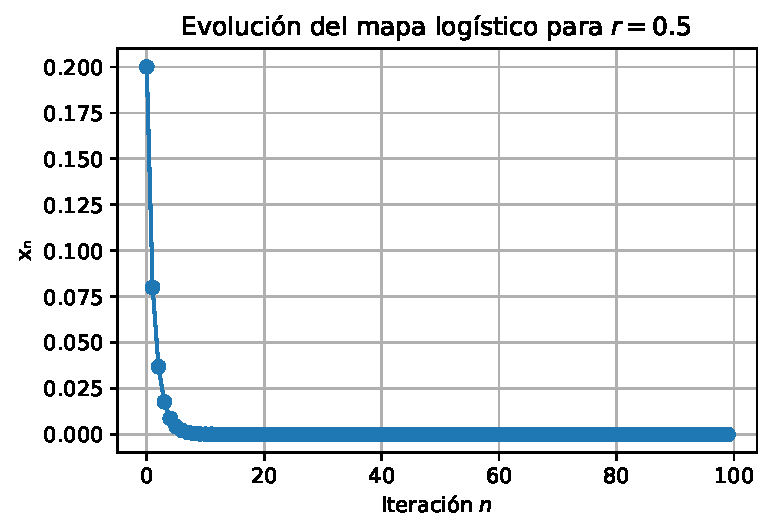
\includegraphics[keepaspectratio]{01-logistica/mapa-logistico_files/figure-pdf/cell-2-output-1.pdf}}

Para valores de \(r\) entre 1 y 3, el valor final de \(x_n\) tiende a un
punto estable

\pandocbounded{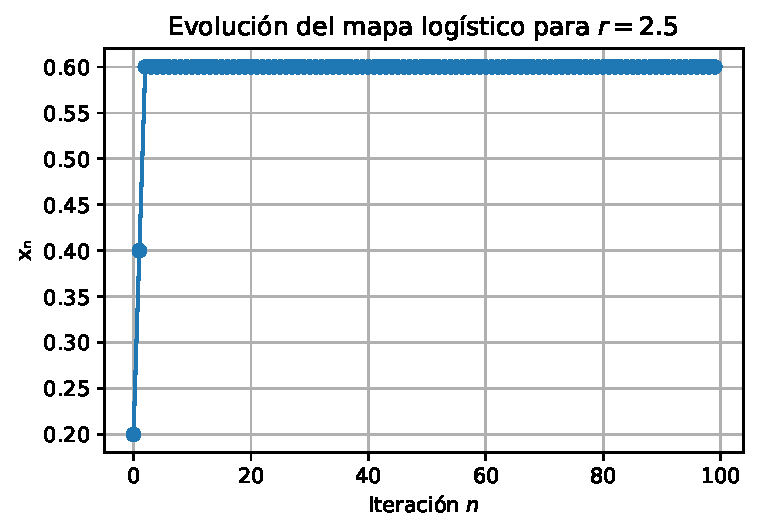
\includegraphics[keepaspectratio]{01-logistica/mapa-logistico_files/figure-pdf/cell-3-output-1.pdf}}

Para valores de \(r\) entre 3 y 3.449, el valor final de \(x_n\) tiende
a dos puntos estables. Es decir, la población tiene un número de
elementos alternantes, que se podría deber a la escasez/abundancia
periódica de recursos.

\pandocbounded{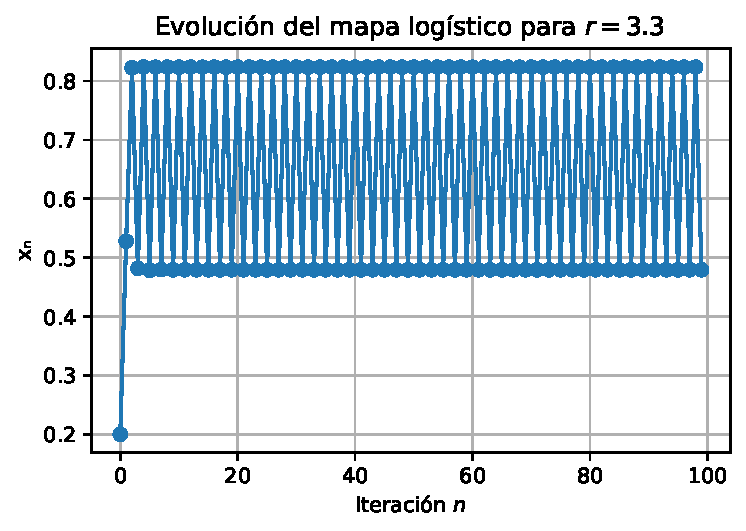
\includegraphics[keepaspectratio]{01-logistica/mapa-logistico_files/figure-pdf/cell-4-output-1.pdf}}

Para valores de \(r\) entre 3 y 3.544, el valor final de \(x_n\) tiende
a cuatro puntos estables. Es curioso ver como la población final alterna
entre 4 números distintos de individuos.

\pandocbounded{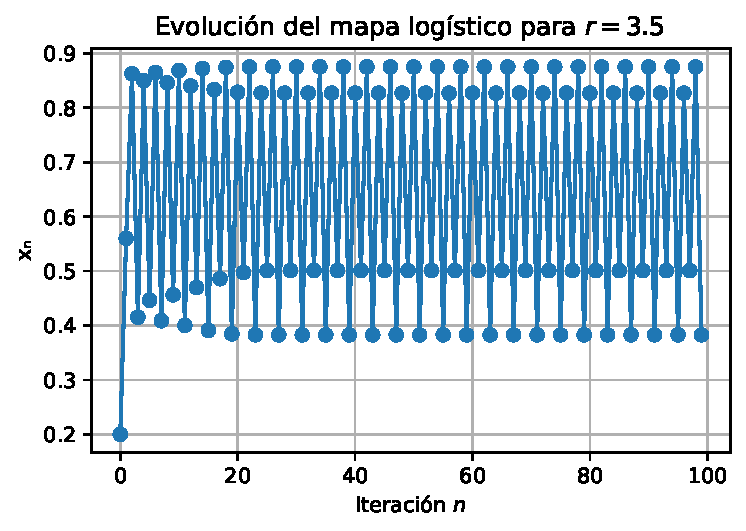
\includegraphics[keepaspectratio]{01-logistica/mapa-logistico_files/figure-pdf/cell-5-output-1.pdf}}

Y a partir de \(r = 3.56995\) no hay ningún punto estable. Se dice que
el sistema en este punto se convierte en caótico

\pandocbounded{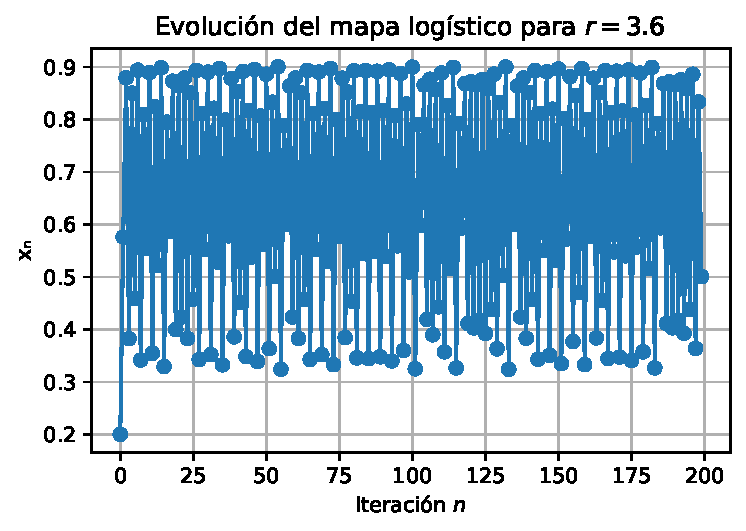
\includegraphics[keepaspectratio]{01-logistica/mapa-logistico_files/figure-pdf/cell-6-output-1.pdf}}

Curioso, ¿verdad?. En la siguiente sección podrás experimentar con
diferentes valores de r y diferentes valores iniciales, para ver cuál es
el estado final del sistema. Después en sucesivas secciones, iremos
explicando formalmente con ayuda de las matemáticas por qué ocurre ésto.

\chapter{Diagrama de telaraña}\label{diagrama-de-telarauxf1a}

\section{Introducción}\label{introducciuxf3n-2}

En sistemas discretos iterativos, un ``diagrama cobweb'' o ``diagrama de
telaraña'' es una representación gráfica que ilustra cómo evoluciona la
secuencia \[
x_{n+1} = f(x_n)
\] paso a paso. Facilita la visualización de convergencia, ciclos y
caos.

\section{Construcción del diagrama
Cobweb}\label{construcciuxf3n-del-diagrama-cobweb}

\begin{enumerate}
\def\labelenumi{\arabic{enumi}.}
\tightlist
\item
  Dibujamos las curvas:

  \begin{itemize}
  \tightlist
  \item
    \(y = f(x)\)
  \item
    \(y = x\)\\
  \end{itemize}
\item
  Partimos de un valor inicial \(x_0\) en el eje horizontal.\\
\item
  Trazamos verticalmente desde \((x_0,0)\) hasta
  \(\bigl(x_0, f(x_0)\bigr)\).\\
\item
  Desde \(\bigl(x_0, f(x_0)\bigr)\) traza horizontalmente hasta la recta
  \(y=x\), llegando a \(\bigl(f(x_0), f(x_0)\bigr)\). Este valor es
  \(x_1\).\\
\item
  Repite el proceso usando \(x_1\) para obtener \(x_2\), y así
  sucesivamente.
\end{enumerate}

Al unir los segmentos verticales y horizontales se forma la ``telaraña''
que muestra la evolución \(x_0 \to x_1 \to x_2 \to \dots\). Así vemos la
evolución del sistema.

\section{¿Para qué sirve?}\label{para-quuxe9-sirve}

\begin{itemize}
\tightlist
\item
  \textbf{Convergencia a punto fijo}: si la telaraña se aproxima a un
  punto de intersección entre \(y=f(x)\) y \(y=x\). En la siguiente
  sección analizaremos el término ``punto fijo''
\item
  \textbf{Detección de ciclos}: patrones periódicos (por ejemplo, saltos
  entre dos puntos indican un ciclo de periodo 2).\\
\item
  \textbf{Observación de caos}: en funciones no lineales como el mapa
  logístico, con ciertos parámetros la telaraña no se estabiliza y
  refleja sensibilidad a condiciones iniciales.
\end{itemize}

Aquí dejo un diagrama interactivo, en el que se observan la función
logística \(y=f(x)=rx(x-1)\), la función \(y = x\), y el diagrama de
telaraña.

El usuario puede jugar con el valor de \(r\) y de \(x_0\) (el valor
inicial de población), y ver la evolución de la población después de 100
iteraciones del mapa logístico.

\begin{verbatim}
Unable to display output for mime type(s): text/html
\end{verbatim}

\chapter{Puntos fijos de una
función}\label{puntos-fijos-de-una-funciuxf3n}

\section{¿Qué es un punto fijo?}\label{quuxe9-es-un-punto-fijo}

Un \textbf{punto fijo} de una función \(f\) es un valor \(x^*\) que
satisface \[x^* = f(x^*)\]

Intuitivamente, si comenzamos en \(x^*\) y aplicamos la función, nos
quedamos en el mismo punto. En la sección anterior vimos que en el
diagram interactivo graficábamos también la función \(y=x\). Si nuestra
función \$f(x)=x'' cruza en algún momento la función \(y=x\), entonces
tenemos un punto fijo en nuestra función.

La pregunta que hay que hacerse, es la siguiente. Si hacemos iteraciones
sucesivas de nuestro mapa/función, ¿convergemos a un punto fijo?. Para
responder esta cuestión, vamos a hacer uso de la derivada de la función
que estamos estudiando.

\section{Estudio formal de la
convergencia}\label{estudio-formal-de-la-convergencia}

Para ver si la sucesión \(x_n\) converge al punto fijo \(x^*\) que
define la ecuación \(x^* = f(x^*)\), en primer lugar vamos a definir el
\textbf{error}: \[
e_n = x_n - x^*,
\] Es decir, \(e_n\) es lo que dista el resultado en la iteración \(n\)
de la sucesión.

La función \(f\) se puede aproximar alrededor de \(x^*\) por medio de su
derivada primera: \[
f(x_n) \approx f(x^*) + f'(x^*)\,(x_n - x^*) 
\]

y usando \(f(x^*)=x^*\), obtenemos \[
e_{n+1} \approx x_{n+1} - x^* = f'(x^*)\,e_n 
\]

Si \(\lvert f'(x^*)\rvert < 1\), entonces
\(\lvert e_{n+1}\rvert < \lvert e_n\rvert\) y por tanto
\(\lvert e_n\rvert\to0\), garantizando que \(x_n\to x^*\).

\section{\texorpdfstring{Ejemplo:
\(f(x)=\cos(x)\)}{Ejemplo: f(x)=\textbackslash cos(x)}}\label{ejemplo-fxcosx}

Si algún día te aburres, coge una calculadora y empieza a apretar
sucesivas veces la función coseno. Verás que acabarás teniendo en el
display de la calculadora el valor 0.739. No es magia. El valor
\(x^* \approx 0.739085\) es el punto fijo de la función coseno.

Veamoslo más formalmente. Consideremos la iteración \[
x_{n+1} = \cos(x_n), \quad x_0 = 0.
\]

Los primeros valores son: \[
\begin{aligned}
x_1 &= \cos(0)=1,\\
x_2 &= \cos(1)\approx0.540302,\\
x_3 &= \cos(x_2)\approx0.857553,\\
x_4 &= \cos(x_3)\approx0.654290,\\
x_5 &= \cos(x_4)\approx0.793480,\\
x_6 &= \cos(x_5)\approx0.701369,\\
x_7 &= \cos(x_6)\approx0.763960,\\
x_8 &= \cos(x_7)\approx0.722102,\\
x_9 &= \cos(x_8)\approx0.750417,\\
x_{10} &= \cos(x_9)\approx0.731404,\\
\end{aligned}
\]

Vemos que los valores van oscilando, pero rápidamente se aproximan al
punto fijo \[
x^* \approx 0.739085,
\] que satisface \(x^* = \cos(x^*)\) (la ecuación \(x^* = \cos(x^*)\) no
tiene solución en forma de fórmula elemental, pues es una ecuación
transcendental).

Además, la derivada en este punto es menor que 1, lo que confirma que es
un punto de atracción de la función. \[
f'(x) = -\sin(x),
\quad
\lvert f'(x^*)\rvert = \lvert\sin(x^*)\rvert < 1,
\] por lo que la iteración converge a \(x^*\).

Si vuelves a la sección anterior, verás que para valores de \(r\) entre
1 y 3, el mapa logístico converge al punto fijo de la función
logísitica. Siempre, independientemente del valor de \(x_0\) que elijas.

Curiosamente, a partir de \(r=3\) la derivada de la función logística en
el punto de corte con \(y=x\) pasa a tener un valor mayor en valor
absoluto que 1, por lo que en este momento el punto de corte deja de ser
un punto fijo.

En la siguiente sección, calcularemos formalmente los puntos fijos de la
función logística y estudiaremos formalmente como se comporta la
sucesión.

\chapter{Estudio formal del mapa
logístico}\label{estudio-formal-del-mapa-loguxedstico}

En los siguientes apartados vamos a desentrañar desde un punto de vista
matemático como se comporta el mapa logístico. Ya hemos visto en los
apartados anteriores, vía simulación, que el comportamiento es muy
errático dependiendo del valor de \(r\). Veamos por qué.

Para empezar veremos la función logística y la analizaremos como
haríamos con cualquier otra función para ver su forma. Para ello,
recurrimos a las técnicas habituales de analisis de funciones.

\section{Dominio y ceros}\label{dominio-y-ceros}

\begin{itemize}
\tightlist
\item
  Por definición, el \textbf{Dominio} es: \(0 \le x \le 1\)\\
\item
  En este dominio los \textbf{Ceros} de la función están en:

  \begin{itemize}
  \tightlist
  \item
    \(f(0) = r \cdot 0 \cdot (1-0) = 0\)\\
  \item
    \(f(1) = r \cdot 1 \cdot (1-1) = 0\)
  \end{itemize}
\end{itemize}

\section{Derivada y monotonía}\label{derivada-y-monotonuxeda}

Para conocer los máximos y mínimos primero hemos de calcular la
derivada,

\begin{itemize}
\tightlist
\item
  Derivada:\\
  \[f'(x) = r(1 - 2x)\]\\
\item
  La derivada tiene una raíz en \(x=1/2\), independientemente del valor
  de \(r\). Por lo tanto, el signo de \(f'(x)\):

  \begin{itemize}
  \tightlist
  \item
    Si \(0 \le x < \tfrac12\), entonces \(f'(x) > 0\) ⇒
    \textbf{creciente}\\
  \item
    Si \(x = \tfrac12\), entonces \(f'(x) = 0\)\\
  \item
    Si \(\tfrac12 < x \le 1\), entonces \(f'(x) < 0\) ⇒
    \textbf{decreciente}
  \end{itemize}
\end{itemize}

De acuerdo al estudio de la derivada, tenemos un punto crítico en
\(x = \tfrac12\). Puesto que la derivada pasa a ser creciente a
decreciente en este punto, tenemos un máximo. La función, pues, tiene un
valor máximo:\\
\[f\bigl(\tfrac12\bigr) = \frac{r}{4}\]

Observar que si \(r>4\) entonces el máximo de la función es mayor que 1.
Esto no puede darse, ya que la funcíón logística normaliza los recursos
máximos disponibles a 1. Por lo tanto, para que no se excedan (cosa que
no puede ocurrir físicamente), el valor de r siempre se establece por
debajo de 4.

\section{Concavidad}\label{concavidad}

\begin{itemize}
\tightlist
\item
  Segunda derivada:\\
  \[f''(x) = -2r\]\\
\item
  Como \(r>0\), \(f''(x)<0\) en todo el dominio ⇒ \textbf{cóncava hacia
  abajo}
\end{itemize}

\section{Rango de la función}\label{rango-de-la-funciuxf3n}

De acuerdo, al estudio anterior, la función es siempre positiva, con
valores entre \(0\) y \(\tfrac{r}{4}\)

Si vamos a la sección con el diagrama de telaraña, veremos efectivamente
esta forma de la función.

\section{Resumen gráfico}\label{resumen-gruxe1fico}

\begin{itemize}
\tightlist
\item
  Parábola invertida con vértice en
  \(\bigl(\tfrac12,\tfrac{r}{4}\bigr)\)\\
\item
  Crece de \(x=0\) a \(x=\tfrac12\), luego decrece hasta \(x=1\)
\end{itemize}

\chapter{Término genérico del mapa
logístico}\label{tuxe9rmino-genuxe9rico-del-mapa-loguxedstico}

En las sucesiones aritméticas y geométricas es fácil expresar el termino
enésimo de la sucesión en función del primer término de la misma.
Veamos:

Término general de la sucesión aritmética

\[a_n = a_1 + (n-1)d\] donde: - \(a_1\) es el primer término. - \(d\) es
la diferencia común. - \(n\) es la posición del término.

Término general de la sucesión geométrica

\[a_n = a_1 \cdot r^{\,n-1}\] donde: - \(a_1\) es el primer término. -
\(r\) es la razón común. - \(n\) es la posición del término.

¿Podemos hacer lo mismo con el mapa logístico?. Hagamos las primeras
iteraciones.

\[
x_1 = r\,x_0\,(1 - x_0)
\]

\[
x_2 = r^2\,x_0\,(1 - x_0)\,\bigl(1 - r\,x_0\,(1 - x_0)\bigr)
\]

\[
x_3 = r^3\,x_0\,(1 - x_0)\,
\bigl(1 - r\,x_0\,(1 - x_0)\bigr)\,
\bigl(1 - r^2\,x_0\,(1 - x_0)\,\bigl(1 - r\,x_0\,(1 - x_0)\bigr)\bigr)
\]

\[
x_4 = r^4\,x_0\,(1 - x_0)\,
\bigl(1 - r\,x_0\,(1 - x_0)\bigr)\,
\bigl(1 - r^2\,x_0\,(1 - x_0)\,\bigl(1 - r\,x_0\,(1 - x_0)\bigr)\bigr)\,
\bigl(1 - r^3\,x_0\,(1 - x_0)\,\bigl(1 - r\,x_0\,(1 - x_0)\bigr)\,\bigl(1 - r^2\,x_0\,(1 - x_0)\,\bigl(1 - r\,x_0\,(1 - x_0)\bigr)\bigr)\bigr)
\]

\[
\begin{aligned}
x_5 =\;& r^5\,x_0\,(1 - x_0)\,
\bigl(1 - r\,x_0\,(1 - x_0)\bigr)\,
\bigl(1 - r^2\,x_0\,(1 - x_0)\,\bigl(1 - r\,x_0\,(1 - x_0)\bigr)\bigr)\\
&\times\;\bigl(1 - r^3\,x_0\,(1 - x_0)\,\bigl(1 - r\,x_0\,(1 - x_0)\bigr)\,\bigl(1 - r^2\,x_0\,(1 - x_0)\,\bigl(1 - r\,x_0\,(1 - x_0)\bigr)\bigr)\bigr)\\
&\times\;\bigl(1 - r^4\,x_0\,(1 - x_0)\,\bigl(1 - r\,x_0\,(1 - x_0)\bigr)\,\bigl(1 - r^2\,x_0\,(1 - x_0)\,\bigl(1 - r\,x_0\,(1 - x_0)\bigr)\bigr)\,\bigl(1 - r^3\,x_0\,(1 - x_0)\,\bigl(1 - r\,x_0\,(1 - x_0)\bigr)\,\bigl(1 - r^2\,x_0\,(1 - x_0)\,\bigl(1 - r\,x_0\,(1 - x_0)\bigr)\bigr)\bigr)\bigr)
\end{aligned}
\]

Como podemos ver, sí que podemos ir expresando los sucesivos términos en
función de solamente \(x_0\) y de \(r\), pero a medida que iteramos, la
expresión se vuelve muy complicada. A pesar de todo, hay que destacar
que la función es \textbf{puramente determinista}. Es decir, se podría
formular el valor de la iteración enésima en función de los valores de
\(x_0\) y de \(r\).

\chapter{Estabilidad del mapa
logístico}\label{estabilidad-del-mapa-loguxedstico}

\section{Puntos fijos}\label{puntos-fijos}

Tal y como habíamos visto anteriormente, un \textbf{punto fijo} \(x^*\)
satisface:

\[
 f(x^*) = x^*.
\]

Para encontrar los puntos fijos de la función logística, resolvemos: \[
r\,x\,(1 - x) = x.
\] Llevando todos los términos a un lado: \[
r\,x\,(1 - x) - x = 0
\quad\Longrightarrow\quad
x\bigl(r\,(1 - x) - 1\bigr) = 0.
\] De aquí se obtienen dos soluciones: \[x_1 = 0\] y \(x_2\) tal que
\(r\,(1 - x_2) - 1 = 0\), es decir: \[
  1 - x_2 = \frac{1}{r}
  \;\Longrightarrow\;
  x_2 = 1 - \frac{1}{r}.
  \]

\section{Evaluación de la derivada en los puntos
fijos}\label{evaluaciuxf3n-de-la-derivada-en-los-puntos-fijos}

La derivada de la función logística es:

\[
 f'(x) = r(1 - 2x).
\]

Y además, de la sección sobre los puntos fijos sabemos que un punto fijo
es estable si \(\lvert f'(x^*)\rvert < 1\).

\begin{itemize}
\tightlist
\item
  \textbf{En \(x^*_1=0\):} \(f'(0)=r\). Estable si \(0 < r < 1\). Es
  decir, para valores de \(r\) comprendidos entre 0 y 1, el valor de
  \(x=0\) es un punto fijo. Lo que ocurre es bien sencillo. Como ya
  comentamos anteriormente, puesto que la población va decreciendo tras
  cada iteración, acaba convergiendo en \(x=0\). Gráficamente también es
  fácil verlo. Si vamos al diagrama de telaraña, y ponemos un \(r<1\),
  veremos que la función lógistica solamente toca a la recta \(y=x\) en
  \(x=0\)
\item
  \textbf{En \(x^*_2=1-1/r\):} \(f'(x^*_2)=2-r\). Estable si
  \(\lvert2-r\rvert<1\) → \(1 < r < 3\). Aquí vemos que el mapa
  logístico converge a un punto, que es el punto fijo. Es lo que
  habíamos visto ya en las soluciones. De nuevo, animo al lector a
  probarlo en el diagrama de telaraña interactivo. Con cualquier valor
  de \(x_0\) que pongan para valores de \(r\) entre 1 y 3, siempre se
  convergerá a un punto que es \(x^*_2=1-1/r\) .
\end{itemize}

Tal y como se muestra en la siguiente figura, a medida que el factor de
crecimiento de la población crece, el número final de individuos aumenta
de forma constante. Como vemos, el valor final de población, siempre
está por debajo del valor máximo de la función logística. Solmente
coincide el valor final con el máximo en r=2. ¿Qué quiere decir esto?.
Que la población puede que en las primeras iteraciones alcance el valor
máximo \(r/4\), pero al final se estabilizar en un valor menor que es
igual a \(x^*_2=1-1/r\) .

\pandocbounded{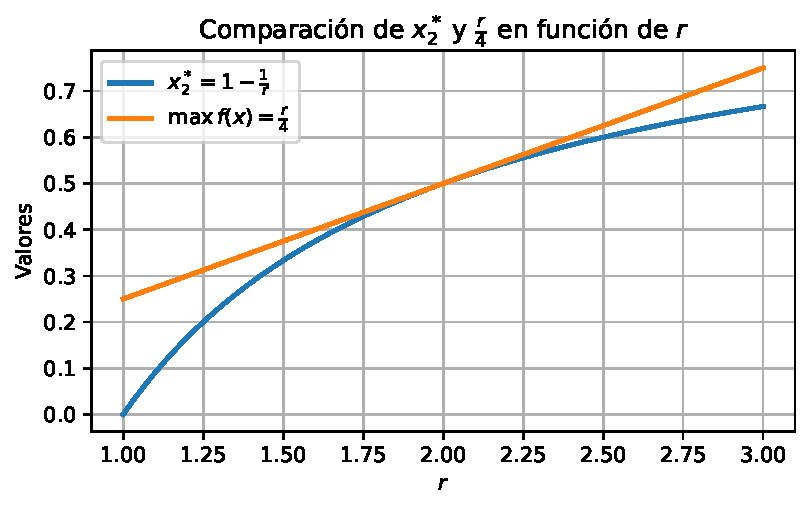
\includegraphics[keepaspectratio]{01-logistica/estable_files/figure-pdf/cell-2-output-1.pdf}}

Añadamos unos gráficos para verlo mejor.

En este primero, vemos para un valor de \(r=0.99\) como la población va
decreciendo iteración tras iteración hasta llegar al punto fijo \(x=0\)

\pandocbounded{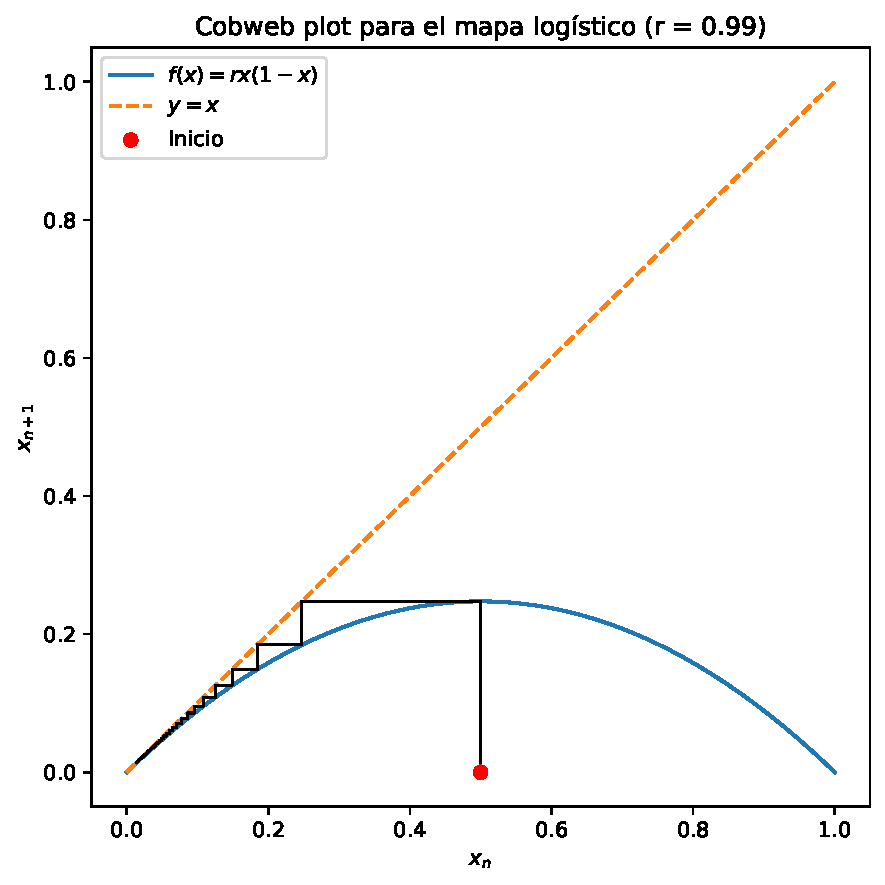
\includegraphics[keepaspectratio]{01-logistica/estable_files/figure-pdf/cell-3-output-1.pdf}}

En este segundo vemos como efectivamente la sucesión converge al punto
fijo (el cruce de la función con la recta \(y=x\)), a pesar de que el
valor de \(r\) está cerca de 3. Pero puesto que sigue siendo menor de 3,
el punto fijo actúa como atractor, y después de 200 iteraciones acaba
convergiendo.

\pandocbounded{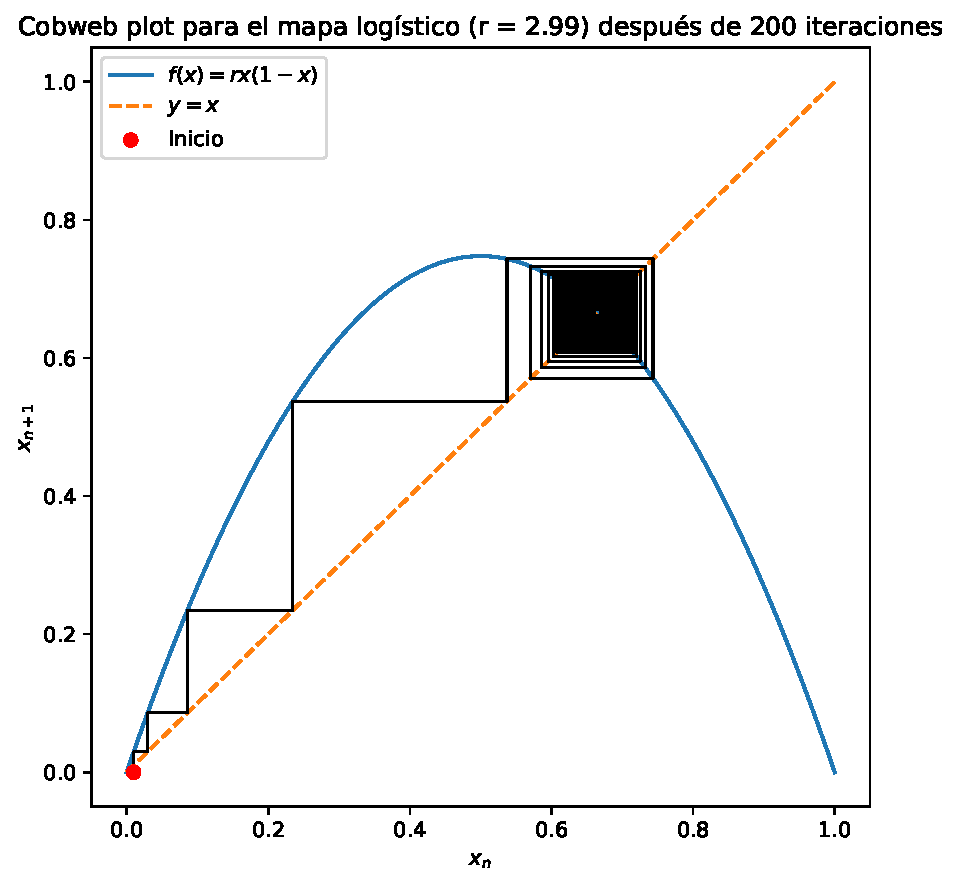
\includegraphics[keepaspectratio]{01-logistica/estable_files/figure-pdf/cell-4-output-1.pdf}}

Pero, ¿qué pasa cuando subimos por encima de \(r=3\)?. Pues que la
derivada en el punto fijo ya no es menor en valor absoluto que 1, y por
lo tanto el punto fijo ya no atrae las iteraciones. El punto fijo, sigue
siendo punto fijo, es decir, si introducimos su valor, la función vuelve
ahí; pero desde cualquier otro punto, ya no va a converger hacia ese
valor. En este caso, vemos que para \(r=3.01\)? la sucesión orbita entre
dos puntos. Es decir, la población final alterna entre dos valores
distintos de individuos. Biológicamente, sucede porque la tasa de
crecimiento \(r\) es lo bastante alta para que, cuando la población se
acerca a la capacidad máxima del entorno, en la siguiente generación
haya un colapso por exceso de competencia (o agotamiento de recursos), y
luego vuelva a recuperarse.

\pandocbounded{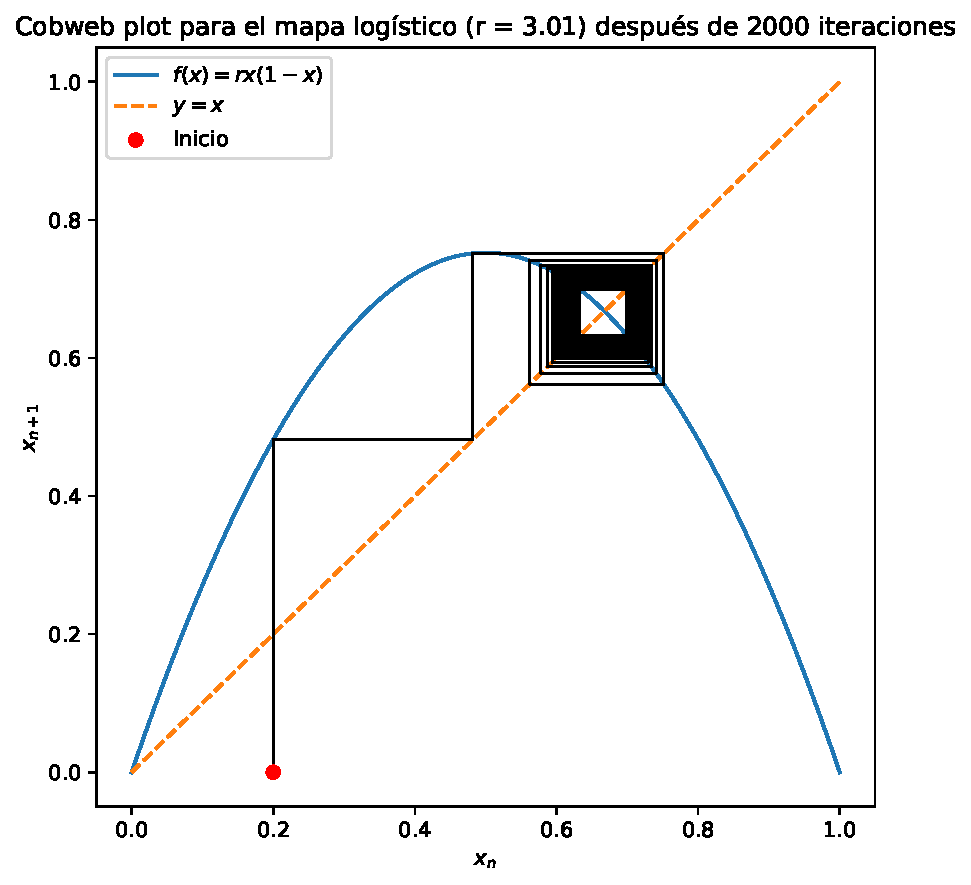
\includegraphics[keepaspectratio]{01-logistica/estable_files/figure-pdf/cell-5-output-1.pdf}}

Aunque el mapa logístico es un modelo muy sencillo, en laboratorio y a
veces en campo se han visto oscilaciones de ``alto-bajo'' de periodo 2
parecidas a las predichas para\(r\approx3\). Algunos ejemplos son:

\begin{itemize}
\item
  \textbf{Moscas de la carne (\emph{Lucilia cuprina})}\\
  En los famosos experimentos de Nicholson sobre poblaciones de moscas
  de la carne, al mantenerlas en condiciones constantes y con alta
  fecundidad, la densidad adulta pasaba de un pico alto un año a un
  valle bajo al siguiente, repitiéndose cada dos generaciones
  \href{https://www.jstor.org/stable/827141?utm_source=chatgpt.com}{Nicholson
  1954},
  \href{https://en.wikipedia.org/wiki/Alexander_John_Nicholson?utm_source=chatgpt.com}{Wikipedia}.
\item
  \textbf{Escarabajos del trigo (\emph{Tribolium confusum})}\\
  Gurney y Nisbet cultivaron colonias de \emph{Tribolium} en el
  laboratorio controlando solo la tasa de natalidad mediante el
  suministro de alimento, y se observó un ciclo bienal: una generación
  con números muy altos seguida de otra bastante más baja, en perfecta
  alternancia
  \href{https://desharnais.sciencecourseware.org/reprints/JAE1987.pdf?utm_source=chatgpt.com}{Gurney
  \& Nisbet 1987},
  \href{https://ojs.openagrar.de/index.php/JKA/article/view/10631/9697?utm_source=chatgpt.com}{Julius
  Kühn-Archiv}.
\item
  \textbf{Daphnia en estanques experimentales}\\
  Algunos estudios con pulgas de agua (\emph{Daphnia}) en estanques
  cerrados, variando la concentración de alimento, han mostrado también
  ciclos aproximados de dos generaciones cuando la tasa de crecimiento
  es lo bastante alta
  \href{https://www.ncbi.nlm.nih.gov/books/NBK2042/?utm_source=chatgpt.com}{NCBI},
  \href{https://www.researchgate.net/publication/31983971_Large-amplitude_cycles_of_Daphnia_and_its_algal_prey_in_enriched_environments?utm_source=chatgpt.com}{ResearchGate}.
\item
  \textbf{Peces capelán (\emph{Mallotus villosus})}\\
  En poblaciones silvestres de capelán del Atlántico Norte, los
  registros de capturas han evidenciado picos de abundancia que tienden
  a repetirse cada dos años, lo cual coincide con su periodo de madurez
  y su ritmo semélparo: tras desovar mueren, lo que promueve ese patrón
  de ``sobrepoblación--agotamiento de recursos'' bienal
  \href{https://en.wikipedia.org/wiki/Capelin?utm_source=chatgpt.com}{Wikipedia},
  \href{https://onlinelibrary.wiley.com/doi/full/10.1002/edn3.415?utm_source=chatgpt.com}{Wiley}.
\end{itemize}

En todos estos casos la dinámica de periodo 2 refleja una
sobrecorrección: tras un año de ``boom'' la población agota alimento o
espacios de puesta, con lo que la siguiente generación cae muy por
debajo de la capacidad de carga, y después se recupera, iniciando de
nuevo el ciclo

En el siguiente apartado, analizaremos formalmente lo que ocurre en la
primera bifurcación del mapa logístico.

\chapter{Primera bifurcación}\label{primera-bifurcaciuxf3n}

Tal y como vimos en la sección anterior cuando \(r > 3\) el valor final
de la sucesión logística alterna entre dos valores finales. Vamos a
hacer un análisis matématico para explicar por qué pasa ésto.

\section{\texorpdfstring{Primera bifurcación: duplicación de período en
\(r = 3\). Análisis
matemático}{Primera bifurcación: duplicación de período en r = 3. Análisis matemático}}\label{primera-bifurcaciuxf3n-duplicaciuxf3n-de-peruxedodo-en-r-3.-anuxe1lisis-matemuxe1tico}

En \(r = 3\), la derivada en el punto fijo \(x^* = 1 - \frac{1}{r}\) se
vuelve \(-1\), lo cual genera una órbita de período 2, tal y como hemos
visto en el apartado anterior.

Surgen dos nuevos puntos \(p\) y \(q\) que no son puntos fijos, sino
puntos de período 2 tales que:

\[
f(p) = q, \quad f(q) = p
\]

Es decir, si al mapa logístico se le alimenta con un valor \(p\), da
como resultado un valor \(q\), que al ser metido otra vez en el mapa
logístico da el valor \(p\) inicial.

Esto significa que:

\[
f(f(p)) = p
\]

Lo cual implica que \(p\) es un punto fijo del mapa iterado \(f^2\)
(esta notación significa la composicion de una función con sigo misma
\(f^2()=f \circ f = f(f())\), no el cuadrado de la función)

Dado que \(f(x) = r x (1 - x)\), podemos escribir:

\[
f(p) = r p (1 - p)
\]

Entonces:

\[
f(f(p)) = r \cdot f(p) \cdot (1 - f(p)) = r \cdot [r p (1 - p)] \cdot \left[1 - r p (1 - p)\right]
\]

Queremos encontrar los puntos de período 2, así que igualamos:

\[
f(f(p)) = p
\]

Hay que observar, que la resolución gráfica es sencilla. Simplemente hay
que dibujar la función \(f^2()=f \circ f = f(f())\) y la función
\(y=x\), y encontrar los cruces de ambas. Se cortarán en dos puntos, que
serán los puntos entre los que alternará el mapa logístico.

Sigamos con la resolución analtíca. Para ello, desarrollamos
completamente \(f(f(p)) = p\):

\[
r^2 p (1 - p)(1 - r p (1 - p)) = p
\]

Pasando todo al mismo lado:

\[
r^2 p (1 - p)(1 - r p (1 - p)) - p = 0
\]

Factorizamos \(p\):

\[
p \left[ r^2 (1 - p)(1 - r p (1 - p)) - 1 \right] = 0
\]

Una de las soluciones es \(p = 0\) (punto fijo trivial), pero las otras
soluciones corresponden a los puntos de período 2.

Expandimos el polinomio:

\[
f(f(p)) = r^2 p (1 - p)(1 - r p (1 - p)) = p
\]

Expandimos paso a paso:

\begin{enumerate}
\def\labelenumi{\arabic{enumi}.}
\tightlist
\item
  \(f(p) = r p (1 - p)\)\\
\item
  \(1 - f(p) = 1 - r p (1 - p)\)\\
\item
  \((1 - p)(1 - r p (1 - p)) = 1 - p - r p (1 - p) + r p^2 (1 - p)\)\\
\item
  Multiplicamos todo por \(r^2 p\)\\
\item
  Resulta en un polinomio de cuarto grado en \(p\)
\end{enumerate}

Este polinomio tiene hasta 4 raíces reales, de las cuales dos
corresponden a los nuevos puntos de período 2. Las otras dos pueden ser
los puntos fijos ya conocidos o raíces no relevantes dinámicamente.

\section{Análisis gráfico}\label{anuxe1lisis-gruxe1fico}

Vamos a proceder al análisis gráfico. Para empezar vamos a poner un mapa
logístico con \(r=2.9\). Sabemos que para este valor la sucesión
converge a un punto. Esto lo vemos porque la función logística corta con
la recta \(y=x\) en un punto cuya pendiente en valor absoluto es menor
que 1, y porque además en ese punto corta también la segunda iterada
\(f \circ f\). La recta \(y=x\) solo corta en un punto a la segunda
iterada, por lo tanto no hay alternancia entre dos puntos.

\pandocbounded{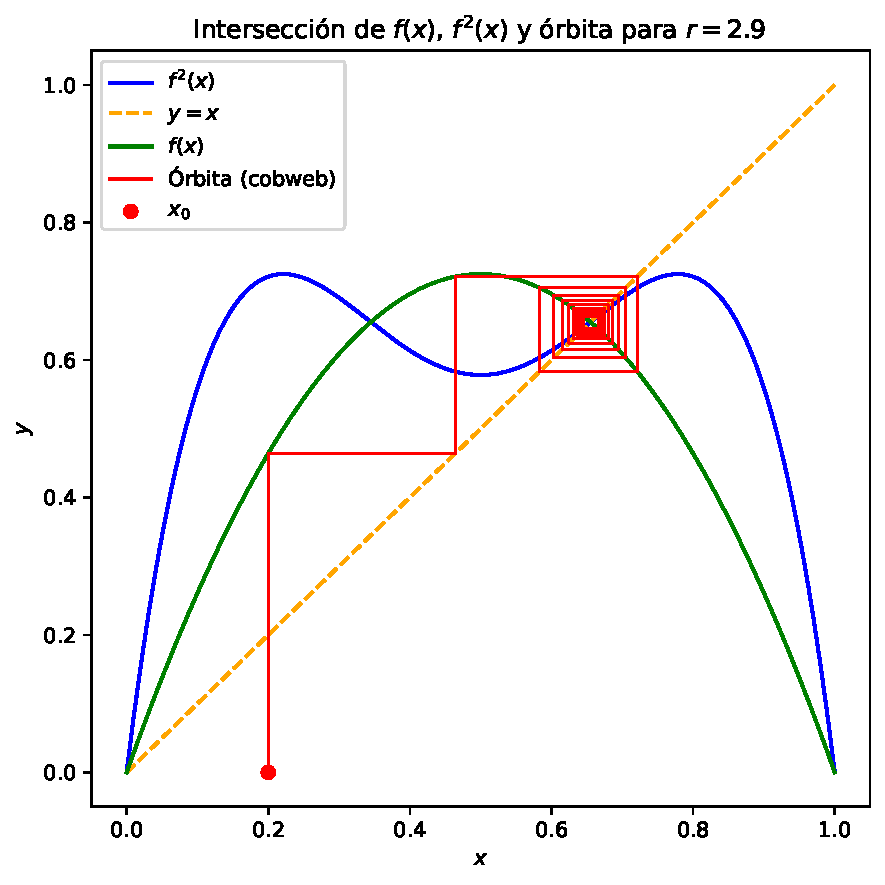
\includegraphics[keepaspectratio]{01-logistica/bifurcaciones_files/figure-pdf/cell-2-output-1.pdf}}

Y ahora veamos lo que pasa cuando \(r=3.2\). En este caso, la segunda
iteración corta con la recta \(y=x\) en dos puntos. Tal y como vemos en
el diagrama de telaraña son estos dos puntos entre los que oscila el
valor final del mapa logístico.

\pandocbounded{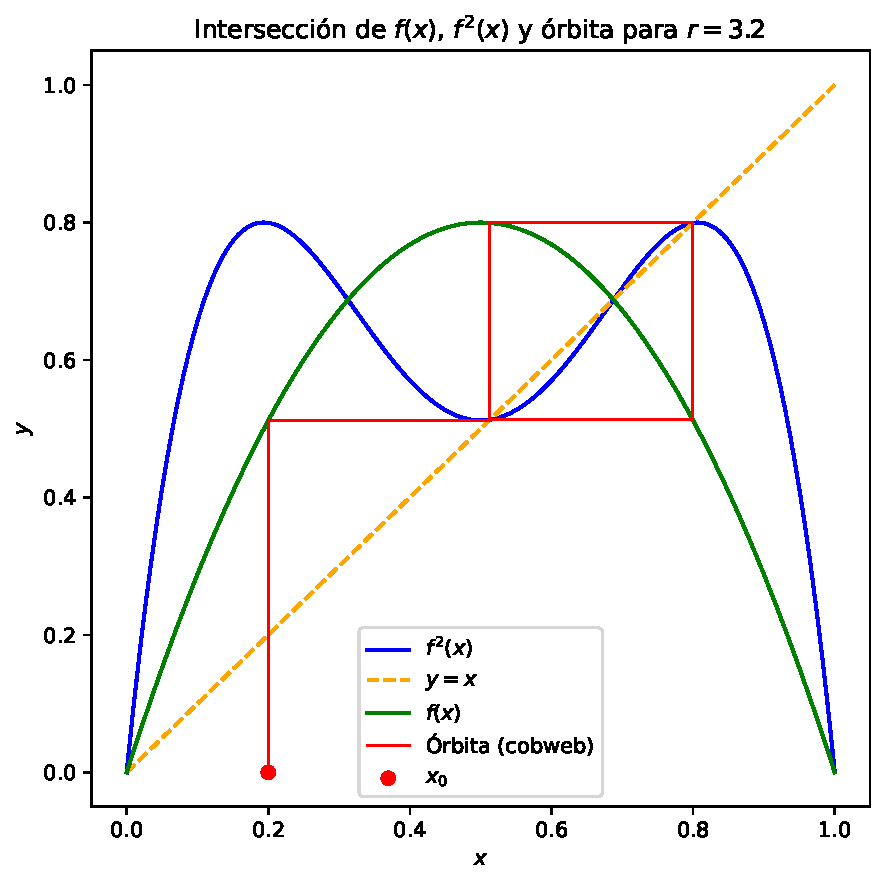
\includegraphics[keepaspectratio]{01-logistica/bifurcaciones_files/figure-pdf/cell-3-output-1.pdf}}

\section{Analisis de estabilidad de la primera
bifurcación}\label{analisis-de-estabilidad-de-la-primera-bifurcaciuxf3n}

En primer lugar, vamos a calcular de nuevo de forma analítica precisa
los puntos en los que se produce la oscilación. La función logística
es\\
\[
f(x) = rx(1 - x),
\]\\
y su iteración doble se define como\\
\[
f^{(2)}(x) = f\bigl(f(x)\bigr).
\]\\
Queremos hallar los valores de \(x\) que satisfacen\\
\[
f^{(2)}(x) = x.
\]

\subsection{\texorpdfstring{Expresión explícita de
\((f^{(2)}(x))\)}{Expresión explícita de (f\^{}\{(2)\}(x))}}\label{expresiuxf3n-expluxedcita-de-f2x}

Primero calculamos\\
\[
f(x) = r x - r x^2.
\]\\
Luego\\
\[
f\bigl(f(x)\bigr)
= r\bigl(f(x)\bigr)\bigl(1 - f(x)\bigr)
= r\bigl(r x - r x^2\bigr)\bigl(1 - (r x - r x^2)\bigr)
\]

Por tanto\\
\[
   f^{(2)}(x)
   = r\,(r x - r x^2)\,(1 - r x + r x^2)
   = r^2\,x\,(1 - x)\,(1 - r x + r x^2)
   \] En vez de expresar la segunda iteración como un polinomio de grado
4, lo dejamos en función de dos monomios y un binomio.

\section{Primera bifurcación: obtención de los puntos fijos de periodo 1
y
2}\label{primera-bifurcaciuxf3n-obtenciuxf3n-de-los-puntos-fijos-de-periodo-1-y-2}

\subsection{Definición de la función y de su iterada
doble}\label{definiciuxf3n-de-la-funciuxf3n-y-de-su-iterada-doble}

La \textbf{función logística} es\\
\[
f(x) = r\,x\,(1 - x)\,.
\]

Su \textbf{segunda iterada} (composición consigo misma) se escribe\\
\[
f^{(2)}(x) = f\bigl(f(x)\bigr)\,.
\]

Queremos resolver\\
\[
f^{(2)}(x) - x = 0,
\]\\
que es un polinomio de grado 4 en (x).

\begin{center}\rule{0.5\linewidth}{0.5pt}\end{center}

\subsection{Puntos de periodo 1 (puntos fijos de
(f))}\label{puntos-de-periodo-1-puntos-fijos-de-f}

Localizamos los puntos de \textbf{periodo 1}, es decir, las raíces de\\
\[
f(x) - x = r\,x\,(1 - x) - x = 0.
\]

Factorizando:\\
\[
r\,x\,(1 - x) - x
= x\bigl[r\,(1 - x) - 1\bigr]
= 0.
\]

De aquí salen dos soluciones:\\
\[
x = 0,
\qquad
x = \frac{r-1}{r}.
\]

\begin{center}\rule{0.5\linewidth}{0.5pt}\end{center}

\subsection{Construcción del polinomio de grado
4}\label{construcciuxf3n-del-polinomio-de-grado-4}

Para la segunda iterada:\\
\[
\begin{aligned}
f^{(2)}(x)
&= r\bigl(f(x)\bigr)\bigl(1 - f(x)\bigr)
= r\bigl(r\,x - r\,x^2\bigr)\bigl[1 - (r\,x - r\,x^2)\bigr]\\[6pt]
&= r^2\,x\,(1 - x)\,(1 - r\,x + r\,x^2).
\end{aligned}
\]

Por tanto,\\
\[
f^{(2)}(x) - x
= r^2\,x\,(1 - x)\,(1 - r\,x + r\,x^2) - x.
\]

\begin{center}\rule{0.5\linewidth}{0.5pt}\end{center}

\subsection{División polinómica para aislar el factor de periodo
2}\label{divisiuxf3n-polinuxf3mica-para-aislar-el-factor-de-periodo-2}

Primero, observemos que si \[x^*\] es un punto fijo de \[f\], es decir,
\[
f(x^*) - x^* = 0,
\] entonces \[
f^{(2)}(x^*) - x^* 
= f\bigl(f(x^*)\bigr) - x^* 
= f(x^*) - x^* 
= 0.
\] Por tanto, toda raíz de \[f(x)-x\] es también raíz de
\[f^{(2)}(x)-x\], lo que en términos de polinomios equivale a afirmar
que \[
f^{(2)}(x)-x
\quad\text{es divisible por}\quad
f(x)-x.
\]

\subsection*{División polinómica paso a paso}

Queremos dividir\\
\[
P(x) \;=\; f^{(2)}(x)-x 
         \;=\; -\,r^3x^4 + 2r^3x^3 - r^2(r+1)x^2 + (r^2-1)x
\] entre\\
\[
D(x) \;=\; f(x)-x 
         \;=\; -\,r\,x^2 + (r-1)x.
\]

\paragraph{Paso 1.}

Dividimos el término de mayor grado de (P(x)) entre el de (D(x)): \[
\frac{-\,r^3x^4}{-\,r\,x^2}
\;=\;
r^2x^2.
\]\\
Multiplicamos y restamos: \[
r^2x^2\cdot D(x)
= -\,r^3x^4 + r^2(r-1)x^3,
\] \[
P(x)-\bigl(r^2x^2\cdot D(x)\bigr)
= (r^3+r^2)x^3 \;-\; r^2(r+1)x^2 \;+\;(r^2-1)x.
\]

\paragraph{Paso 2.}

Dividimos el nuevo término principal entre el de (D(x)): \[
\frac{(r^3+r^2)x^3}{-\,r\,x^2}
\;=\;
-\,(r^2+r)x.
\]\\
Multiplicamos y restamos: \[
-\,(r^2+r)x\cdot D(x)
= -\,(r^3+r^2)x^3 + (r^3-r)x^2,
\] \[
\bigl[(r^3+r^2)x^3 - r^2(r+1)x^2 + (r^2-1)x\bigr]
-
\bigl[-(r^3+r^2)x^3 + (r^3-r)x^2\bigr]
= -\,(r^2+r)x^2 + (r^2-1)x.
\]

\paragraph{Paso 3.}

Dividimos nuevamente: \[
\frac{-\,(r^2+r)x^2}{-\,r\,x^2}
\;=\;
r+1.
\]\\
Multiplicamos y restamos: \[
(r+1)\cdot D(x)
= -\,(r^2+r)x^2 + (r^2-1)x,
\] \[
\bigl[-(r^2+r)x^2 + (r^2-1)x\bigr]
-
\bigl[-(r^2+r)x^2 + (r^2-1)x\bigr]
= 0.
\]

\paragraph{Resultado.}

El cociente es \[
Q(x) \;=\; r^2x^2 \;-\;(r^2+r)x \;+\;(r+1),
\] y el resto es cero.

El \textbf{cociente} resultante es \[
Q(x) \;=\; r^2x^2 \;-\;(r^2+r)x \;+\;(r+1),
\] y el resto es cero, tal como queríamos demostrar.

\subsubsection{Paso 1}\label{paso-1}

\begin{itemize}
\tightlist
\item
  Cociente parcial:\\
  \[
  \frac{-r^3x^4}{-r\,x^2} = r^2x^2.
  \]
\item
  Multiplicamos y restamos → nuevo dividendo.
\end{itemize}

\subsubsection{Paso 2}\label{paso-2}

\begin{itemize}
\tightlist
\item
  Cociente parcial:\\
  \[
  \frac{(r^3+r^2)x^3}{-r\,x^2} = -(r^2+r)x.
  \]
\item
  Multiplicamos y restamos → nuevo dividendo.
\end{itemize}

\subsubsection{Paso 3}\label{paso-3}

\begin{itemize}
\tightlist
\item
  Cociente parcial:\\
  \[
  \frac{-(r^2+r)x^2}{-r\,x^2} = r+1.
  \]
\item
  Multiplicamos y restamos → \textbf{resto cero}.
\end{itemize}

\textbf{Cociente final}:\\
\[
Q(x) = r^2x^2 - (r^2+r)x + (r+1).
\]

\begin{center}\rule{0.5\linewidth}{0.5pt}\end{center}

\subsection{Solución de las raíces de periodo
2}\label{soluciuxf3n-de-las-rauxedces-de-periodo-2}

Resolvemos\\
\[
r^2x^2 - (r^2+r)x + (r+1) = 0
\]\\
con la fórmula cuadrática:

\[
x_{1,2}
= \frac{(r^2+r)\pm\sqrt{(r^2+r)^2 - 4r^2(r+1)}}{2r^2}
= \frac{r+1\pm\sqrt{(r+1)(r-3)}}{2r}.
\]

Así:

\[
x_1 = \frac{r+1 + \sqrt{(r+1)(r-3)}}{2r},
\qquad
x_2 = \frac{r+1 - \sqrt{(r+1)(r-3)}}{2r}.
\]

\begin{quote}
\textbf{Nota:} En (r=3) el discriminante ((r+1)(r-3)) se anula y ambas
raíces confluyen en (x=2/3), coincidiendo con el punto fijo que pierde
estabilidad.
\end{quote}

Obsérvese, que para \(r=3\), no hay dos soluciones, sino una, que
coincide con el punto estable (\(x=2/3\)). Ahora que tenemos la fórmula
de los puntos finales, vamos a ver si estos dos puntos finales son
estables. Para ello haremos lo mismo que para el caso \(1<r<3\) . Es
decir, cuando estábamos en la región estable \(1<r<3\), el punto de
estabilidad final lo daba el cruce que la función logística con la recta
\(y=x\), imponiendo la condición adicional de que el valor absoluto de
la derivada en ese cruce sea menor que 1. Ahora, haremos lo mismo, pero
imponiendo la condición adicional sobre la derivada de la segunda
iteración de la función.

\subsection{\texorpdfstring{Derivada de \(f\) y criterio de
estabilidad}{Derivada de f y criterio de estabilidad}}\label{derivada-de-f-y-criterio-de-estabilidad}

Supongamos que \((x_1,x_2)\) es un ciclo de periodo 2, es decir\\
\[
f(x_1)=x_2,\qquad f(x_2)=x_1.
\]\\
Queremos ver qué pasa si en lugar de empezar exactamente en \(x_1\)
tomamos un punto ``ligeramente'' desviado:\\
\[
x_1 + \delta,
\]\\
con \(\delta\) muy pequeño.

Al aplicar \(f\) alrededor de \(x_1\), usamos la aproximación lineal:

\[
f(x_1 + \delta)
\approx f(x_1) + f'(x_1)\,\delta
= x_2 + f'(x_1)\,\delta.
\]

Así, tras una iteración, nuestro error (desviación) se amplifica o
reduce por el factor \(f'(x_1)\).

Ahora iteramos de nuevo, partiendo de\\
\[
x_2 + f'(x_1)\,\delta.
\]\\
Otra vez linealizamos en torno a \(x_2\):

\[
f\bigl(x_2 + f'(x_1)\,\delta\bigr)
\approx f(x_2) + f'(x_2)\,\bigl(f'(x_1)\,\delta\bigr)
= x_1 + \bigl[f'(x_2)\,f'(x_1)\bigr]\,\delta.
\]

Después de dos pasos (una vuelta completa al ciclo de período 2), la
desviación original \(\delta\) se convierte en

\[
\delta_{\rm nuevo} = f'(x_2)\,f'(x_1)\,\delta.
\]

Por tanto, \textbf{el factor que controla la estabilidad} del ciclo de
período 2 es precisamente

\[
\Lambda = f'(x_1)\,f'(x_2).
\]

\begin{itemize}
\tightlist
\item
  Si \(|\Lambda|<1\), la desviación \(\delta\) tiende a cero y el ciclo
  es \textbf{estable}.\\
\item
  Si \(|\Lambda|>1\), la desviación crece y el ciclo es
  \textbf{inestable}.
\end{itemize}

Veamos otra forma de calcularlo. Formalmente, la derivada de la
composición \(f^{(2)}=f\circ f\) se calcula con la regla de la cadena:

\[
(f^{(2)})'(x)
= f'(f(x))\,f'(x).
\]

Si evaluamos en \(x=x_1\), tenemos:

\[
(f^{(2)})'(x_1)
= f'(f(x_1))\,f'(x_1)
= f'(x_2)\,f'(x_1),
\]

que es exactamente el mismo producto que acabamos de entender con el
argumento de las dos iteraciones sucesivas.

Por lo tanto, el ciclo de periodo 2 es estable si\\
\[
\bigl|f'(x_1)\,f'(x_2)\bigr| < 1.
\]

Vamos a proceder a evaluar el producto de derivadas en los puntos
\(x_1\) y \(x_2\) calculados anteriormente. Recordemos: \[
x_1 = \frac{r+1 + \sqrt{(r+1)(r-3)}}{2r},
\qquad
x_2 = \frac{r+1 - \sqrt{(r+1)(r-3)}}{2r},
\] y \[
f'(x) = r\,(1 - 2x).
\]

\begin{enumerate}
\def\labelenumi{\arabic{enumi}.}
\item
  \textbf{Derivada en (x\_1)}\\
  {[}

  \begin{aligned}
  f'(x_1)
  &= r\Bigl(1 - 2\,x_1\Bigr)
  = r\Bigl(1 - 2\,\frac{r+1 + \sqrt{(r+1)(r-3)}}{2r}\Bigr) \\[6pt]
  &= r\Bigl(1 - \frac{r+1 + \sqrt{(r+1)(r-3)}}{r}\Bigr)
  = r\Bigl(\frac{r - (r+1 + \sqrt{(r+1)(r-3)})}{r}\Bigr) \\[6pt]
  &= r\;\frac{-1 - \sqrt{(r+1)(r-3)}}{r}
  = -1 \;-\;\sqrt{(r+1)(r-3)}.
  \end{aligned}

  {]}
\item
  \textbf{Derivada en (x\_2)}\\
  {[}

  \begin{aligned}
  f'(x_2)
  &= r\Bigl(1 - 2\,x_2\Bigr)
  = r\Bigl(1 - 2\,\frac{r+1 - \sqrt{(r+1)(r-3)}}{2r}\Bigr) \\[6pt]
  &= r\Bigl(1 - \frac{r+1 - \sqrt{(r+1)(r-3)}}{r}\Bigr)
  = r\Bigl(\frac{r - (r+1 - \sqrt{(r+1)(r-3)})}{r}\Bigr) \\[6pt]
  &= r\;\frac{-1 + \sqrt{(r+1)(r-3)}}{r}
  = -1 \;+\;\sqrt{(r+1)(r-3)}.
  \end{aligned}

  {]}
\item
  \textbf{Producto de las derivadas}\\
  {[}

  \begin{aligned}
  f'(x_1)\,f'(x_2)
  &= \bigl(-1 - \sqrt{(r+1)(r-3)}\bigr)
     \bigl(-1 + \sqrt{(r+1)(r-3)}\bigr) \\[6pt]
  &= (-1)^2 \;-\;\bigl(\sqrt{(r+1)(r-3)}\bigr)^2
  = 1 \;-\;(r+1)(r-3) \\[4pt]
  &= 1 - \bigl(r^2 - 2r - 3\bigr)
  = -\,r^2 + 2r + 4.
  \end{aligned}

  {]}
\end{enumerate}

La bifurcación de periodo 2 a periodo 4 ocurre cuando el producto cruza
\(-1\) (al graficar la función \(f \circ f\) se observa que su derivada
se va haciendo negativa en el punto de cruce con \(y=x\) a medida que
aumentamos \(r\) ; por ello no igualamos a +1): \[
-r^2 + 2r + 4 = -1
\quad\Longrightarrow\quad
r^2 - 2r - 5 = 0
\quad\Longrightarrow\quad
r = 1 \pm \sqrt{6}.
\]\\
Despreciando la solución negativa, tomamos\\
\[
r_c = 1 + \sqrt{6} \approx 3.44949.
\]

Por lo tanto, recopilando lo que tenemos hasta ahora:

\begin{itemize}
\tightlist
\item
  Para \(0 < r < 1\) la sucesión tiende a cero
\item
  Para \(1 < r < 3\) la sucesión tiende a un punto final único
\item
  Para \(3 < r < (1 + \sqrt{6})\) tiende a dos puntos que se van
  alternando
\end{itemize}

¿Qué pasará a partir de \(r > 1 + \sqrt{6}\) ?. Podríamos repetir el
análisis que acabamos de realizar. Sin embargo, resulta muy farragoso
matemáticamente, dado que el orden de los polinomios involucrados es muy
grande. Por ello, vamos a recurrir a la simulación numérica en la
siguiente sección.

\chapter{Bifurcaciones sucesivas}\label{bifurcaciones-sucesivas}

En el siguiente diagrama interactivo se muestra el valor final del mapa
logístico para distintos valores de la tasa de crecimiento \(r\). El
usuario puede jugar con los valores de \(r\), el valor inicial de \(x\)
y el número de iteraciones hasta un máximo de 500 iteraciones.

\begin{verbatim}
Unable to display output for mime type(s): text/html
\end{verbatim}

El primer detalle que no pasa desapercibido es ver como los valores
máximos y mínimos están constreñidos entre dos curvas perfectamente
definidas. En la siguiente gráfica se puede apreciar que el máximo que
alcanza para cada valor de \(r\) es precisamente \(r/4\) tal y como
habíamos calculado en la sección en la que hicimos el análisis formal
del mapa logístico. Y su valor mínimo es la iteración del valor máximo,
es decir \(r^2/4(1-r/4)\). Solamente cuando \(r=4\) se cubre todo el
rango de valores desde 0 hasta 1.

\pandocbounded{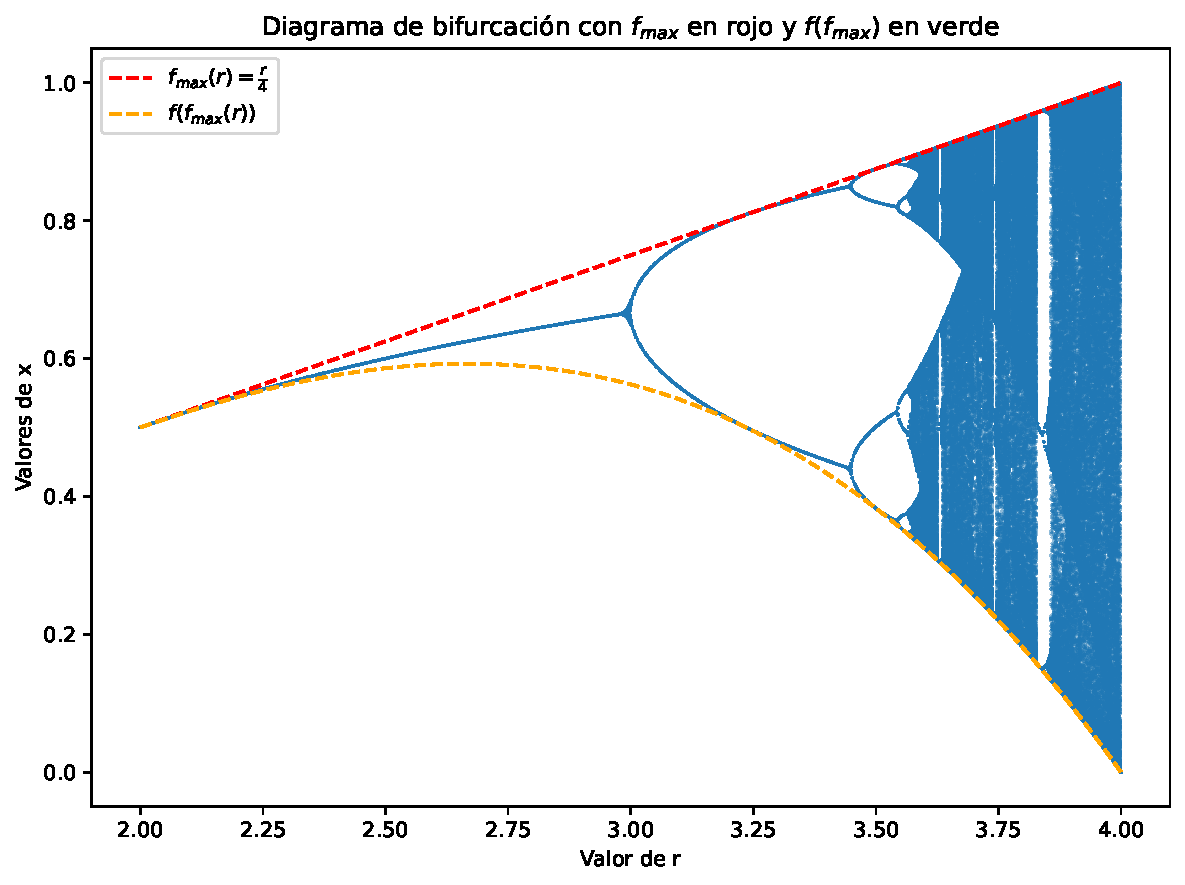
\includegraphics[keepaspectratio]{01-logistica/simulacion_files/figure-pdf/cell-3-output-1.pdf}}

Sigamos con el análisis visual del gráfico. Conforme \(r\) crece,
aparecen bifurcaciones que duplican el periodo sucesivamente:

\begin{itemize}
\tightlist
\item
  \(r_1=3.0\) → periodo 2. Analizada en la sección anterior.
\item
  \(r_2 \approx 3.449\) → periodo 4. Tal y como vimos en la sección
  anterior para \(r = 1 + \sqrt{6}\), la primera bifurcación deja de ser
  estable y vemos que aparece una bifurcación adicional, por lo que el
  valor final del mapa lógístico alterna entre 4 valores finales.
\item
  \(r_3 \approx 3.544\) → periodo 8. Aparece una nueva bifurcación y
  ahora el valor final del mapa lógístico alterna entre 8 valores
  finales.
\end{itemize}

Vamos a hacer un zoom a la zona con \(r\) entre 3.4 y 3.6 para ver que
pasa con más detalle a partir de \(r_3 \approx 3.544\)

\pandocbounded{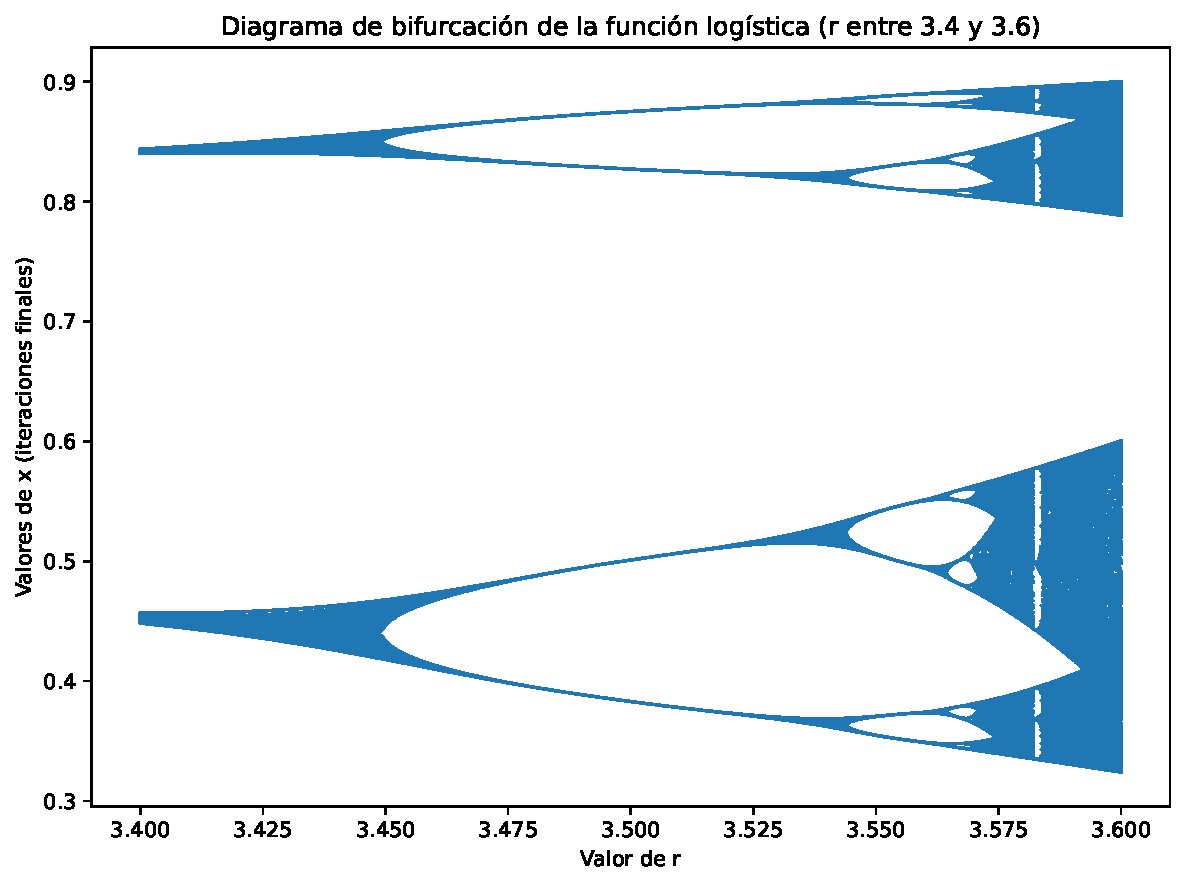
\includegraphics[keepaspectratio]{01-logistica/simulacion_files/figure-pdf/cell-4-output-1.pdf}}

Vemos un montón de bifurcaciones (periodo 2, 4, 8, 16). Vamos a hacer un
zoom adicional a la zona con \(r\) comprendido entre 3.449 y 3.56995.

\pandocbounded{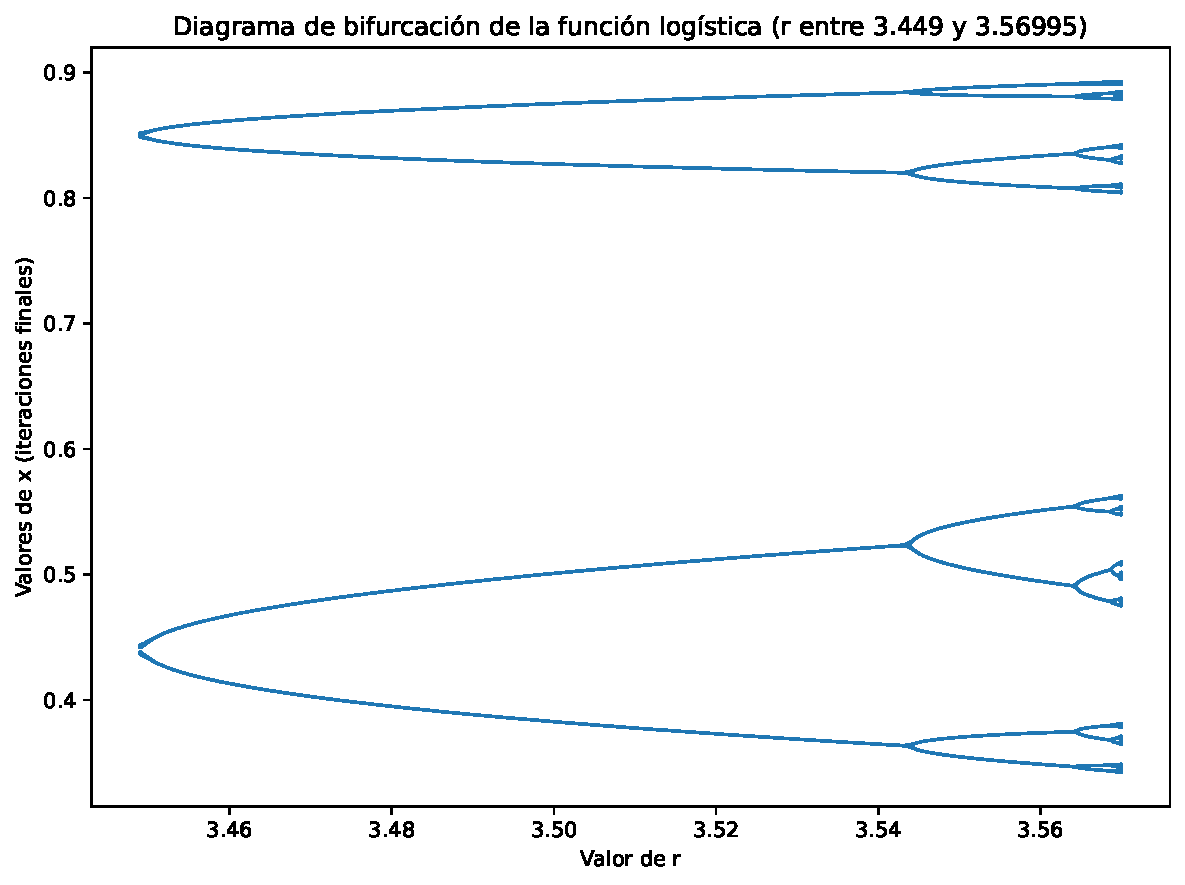
\includegraphics[keepaspectratio]{01-logistica/simulacion_files/figure-pdf/cell-5-output-1.pdf}}

Vemos ahora mejor las primerasbifurcaciones (periodo 2, 4, 8, 16).
Parece que el valor final de la función logística va creando
sucesivamente nuevos ciclos, hasta que llegamos a un valor cercano a
3.57 (3.56995 para ser más exactos). A partid de este valor de \(r\)
dejan de verse claramente oscilaciones periódicas, y pasamos al régimen
caótico. Vamos a hacer un zoom adicional a la zona con \(r\) comprendido
entre 3.56 y 3.575.

\pandocbounded{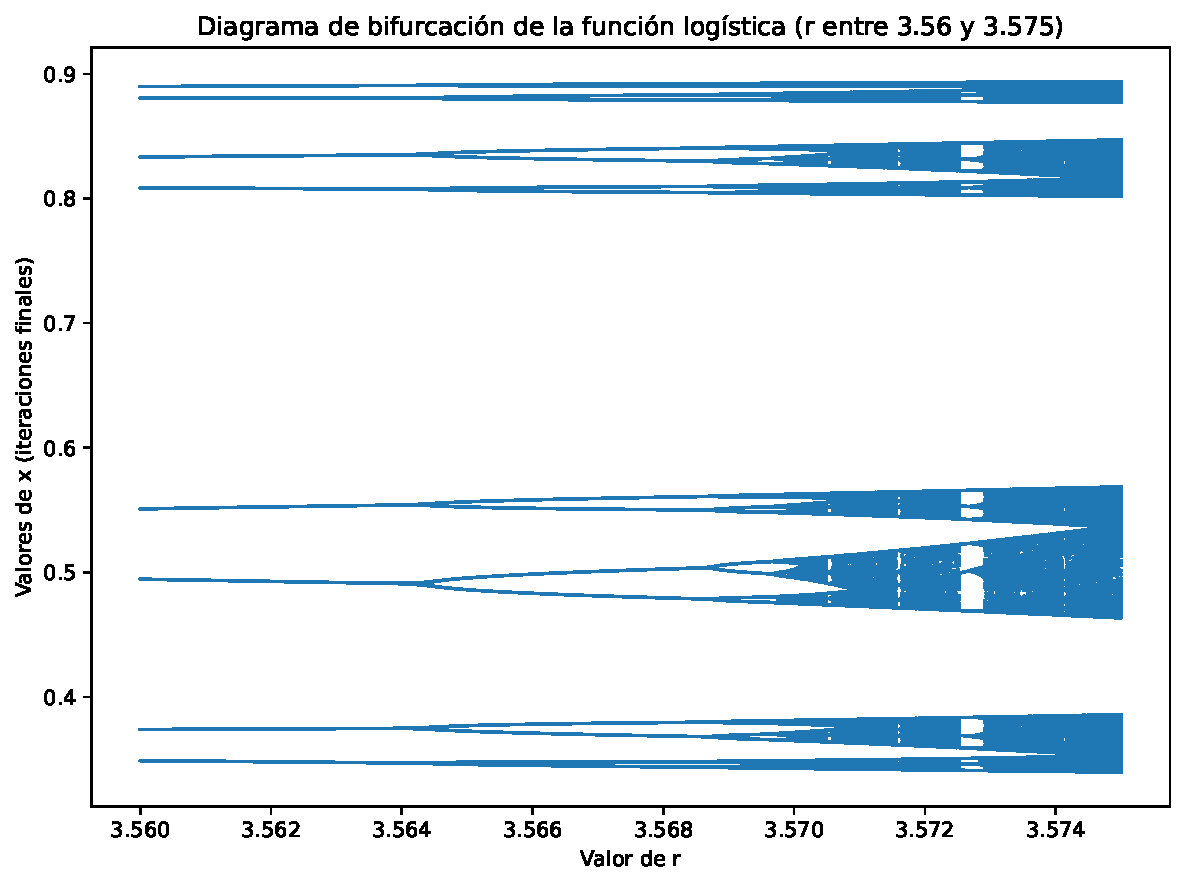
\includegraphics[keepaspectratio]{01-logistica/simulacion_files/figure-pdf/cell-6-output-1.pdf}}

\chapter{Caos}\label{caos}

Como dijimos en la seccíón anterior, a partir de
\(r_\infty \approx 3.56995\), el mapa logístico entra en un
\textbf{régimen caótico}. Para \(r < r_\infty\), aparecían sucesivas
bifurcaciones de periodo \(1 \to 2 \to 4 \to 8 \to \cdots\). En
\(r = r_\infty\), esas bifurcaciones se acumulan y ya no hay ciclos
periódicos finitos: el valor final se vuelve errático. Sin embargo a
medida que vamos observando el mapa aparecen comportamientos extraños.

\section{División en bandas}\label{divisiuxf3n-en-bandas}

Justo tras \(r_\infty\), la zona caótica se \textbf{parte en dos bandas}
disjuntas: en el diagrama de bifurcación aparecen dos hileras de puntos
con un hueco entre ellas.

\pandocbounded{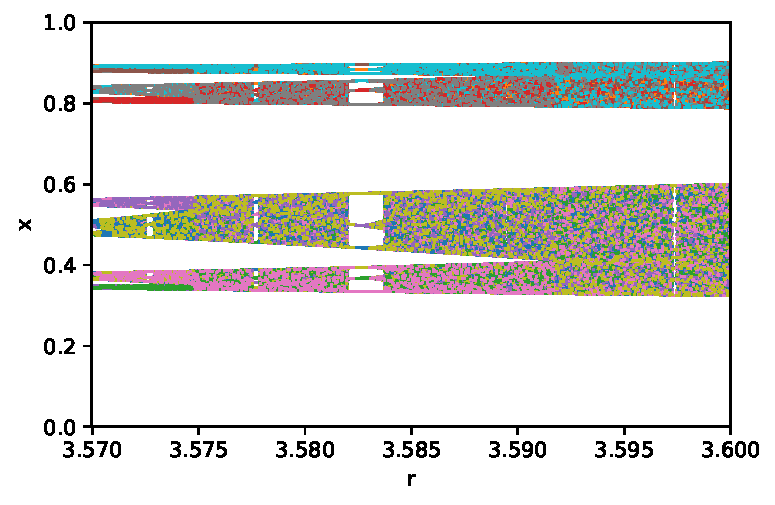
\includegraphics[keepaspectratio]{01-logistica/Caos_files/figure-pdf/cell-2-output-1.pdf}}

A medida que subimos \(r\), esas dos bandas se bifurcan en 4, luego en
8, repitiendo la misma lógica de duplicación pero sobre la estructura
del caos.

\pandocbounded{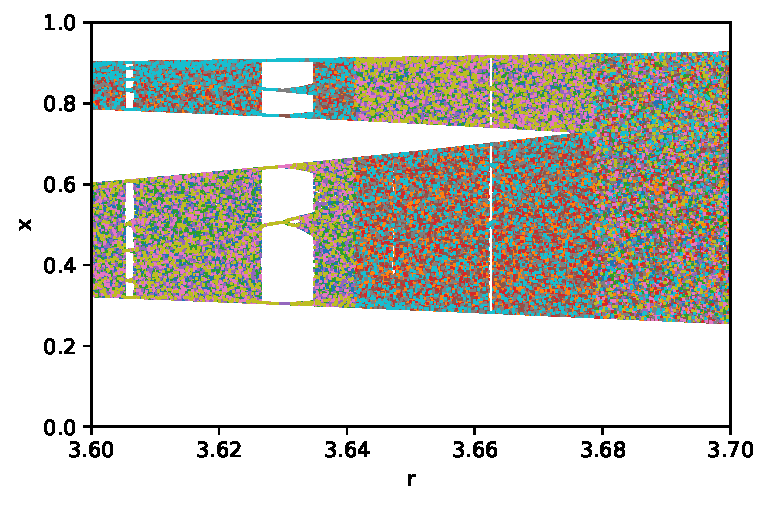
\includegraphics[keepaspectratio]{01-logistica/Caos_files/figure-pdf/cell-3-output-1.pdf}}

\section{Ventanas de periodicidad}\label{ventanas-de-periodicidad}

En medio del caos surgen \textbf{islas} de orden donde aparece un ciclo
estable de periodo \(k\) (por ejemplo, un ciclo de orden 3 alrededor de
\(r\approx3.828\)).

\pandocbounded{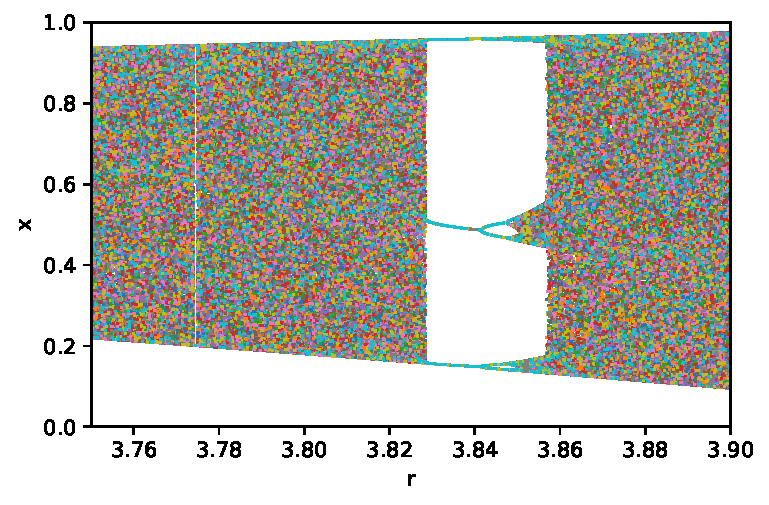
\includegraphics[keepaspectratio]{01-logistica/Caos_files/figure-pdf/cell-4-output-1.pdf}}

Dentro de cada ventana periódica se reproduce una \textbf{mini-cascada}
de duplicación de periodo \(k \to 2k \to 4k \to \cdots\). Lo mismo que
teníamos en la zona \(3 < r < 3.56995\) pero ahora dentro de la zona
caótica. Vemos como el caos da paso de nuevo a las órbitas periódicas

\pandocbounded{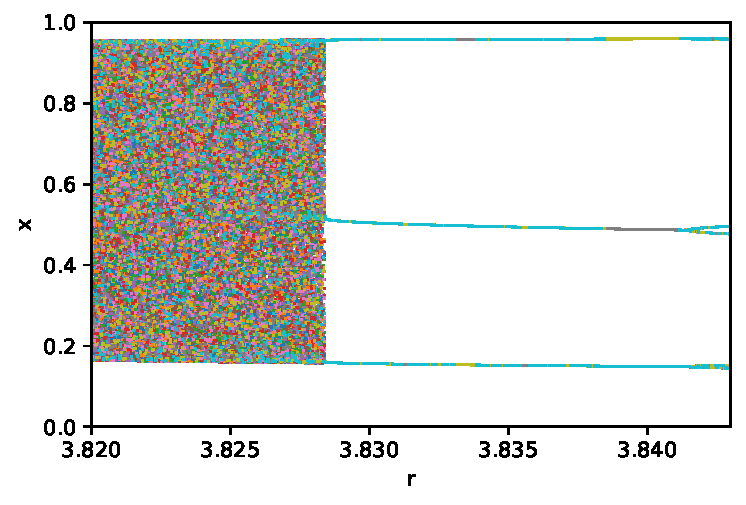
\includegraphics[keepaspectratio]{01-logistica/Caos_files/figure-pdf/cell-5-output-1.pdf}}

\section{Repetición infinita}\label{repeticiuxf3n-infinita}

Las ventanas de periodicidad están \textbf{infinitamente repetidas}: en
cada fragmento de la región caótica, por pequeño que sea, habrá alguna
ventana donde emerja un ciclo estable.

Así vemos como enre 3.73 y 3.76 aparecen un ciclo de período 5.

\pandocbounded{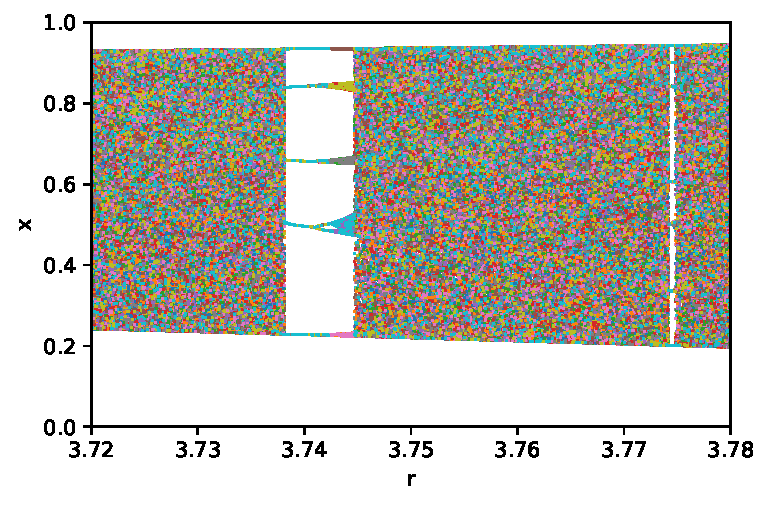
\includegraphics[keepaspectratio]{01-logistica/Caos_files/figure-pdf/cell-6-output-1.pdf}}

Si nos centramos en los valores de x alrededor de 0.5, vemos claramente
el diagrama de bifurcación inicial replicado aquí, con tan solo 1000
iteraciones.

\pandocbounded{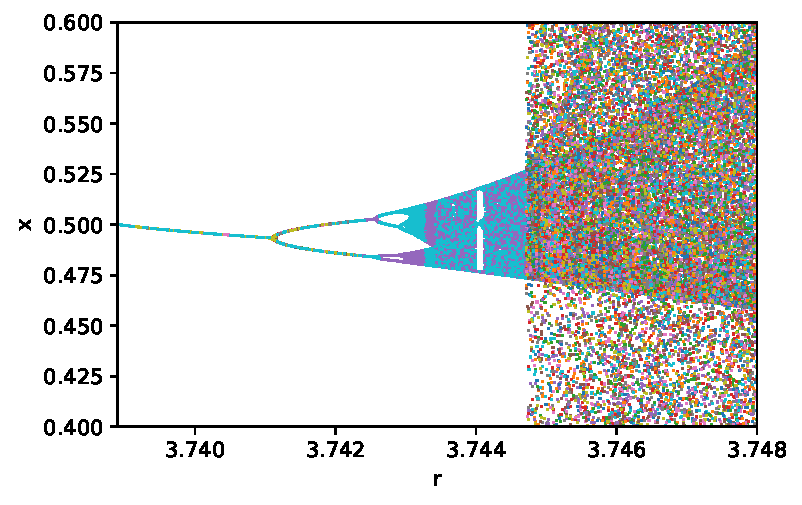
\includegraphics[keepaspectratio]{01-logistica/Caos_files/figure-pdf/cell-7-output-1.pdf}}

Y dentro de esta replicación del diagrama de bifurcación original,
podemos encontrar el ciclo de periodo 5 de nuevo, en los valores de
\(r\) comprendidos entre 3.74431 y 3.74433.

\pandocbounded{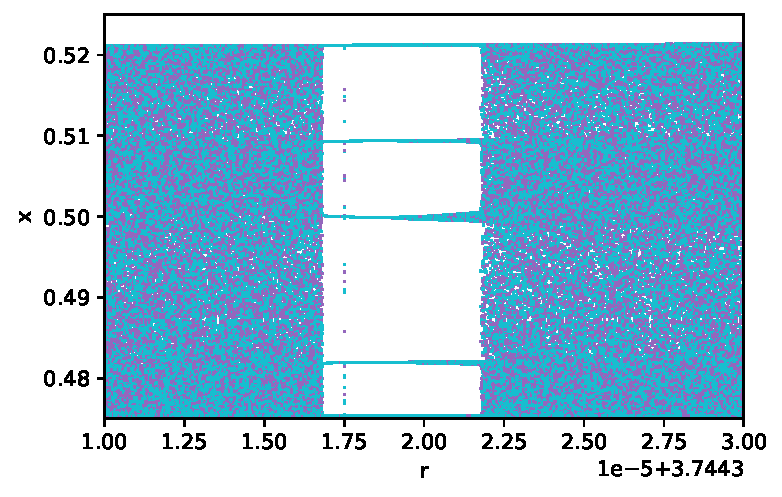
\includegraphics[keepaspectratio]{01-logistica/Caos_files/figure-pdf/cell-8-output-1.pdf}}

Y de nuevo, cogemos la replicación del diagrama de bifurcación original
alrededor de 0.5 y nos encontramos con el ciclo de periodo 5 de nuevo,
en los valores de \(r\) comprendidos entre 3.74432144 y 3.744321455.
Cada vez necesitaremos más iteraciones para apreciar el diagrama de
bifurcación original. De hecho, para plotear esta última gráfica se han
requerido 100.000 iteraciones

\pandocbounded{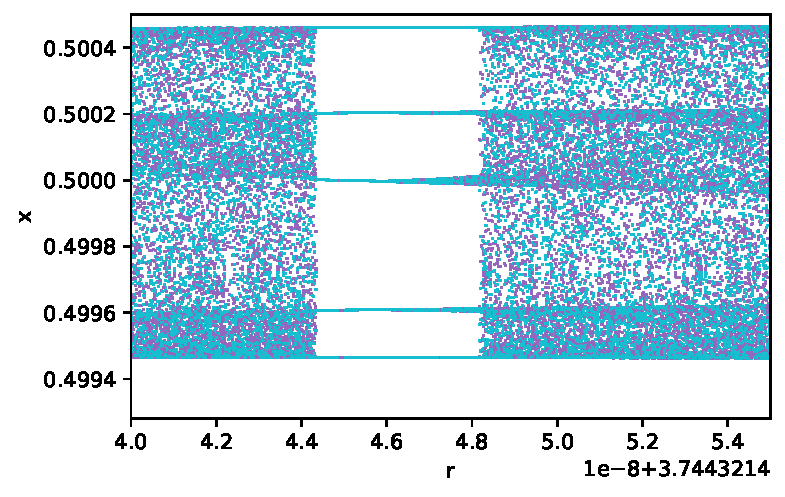
\includegraphics[keepaspectratio]{01-logistica/Caos_files/figure-pdf/cell-9-output-1.pdf}}

Haciendo de nuevo zoom en torno a 0.5, vemos como aparece el diagrama de
bifurcación original, esta vez en los valores de \(r\) comprendidos
entre 3.7443214444 y 3.744321448 , tras 1.000.000 de iteraciones.

\pandocbounded{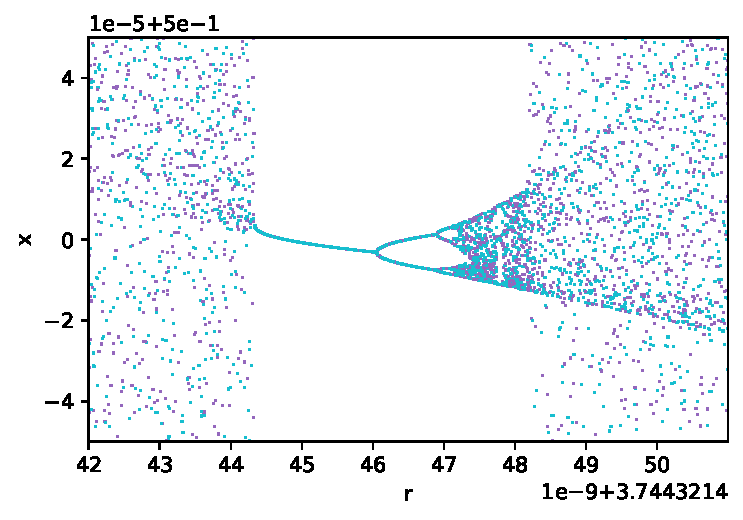
\includegraphics[keepaspectratio]{01-logistica/Caos_files/figure-pdf/cell-10-output-1.pdf}}

Podemos seguir así infinitamente. Lo que hemos encontrado es una
\textbf{estructura fractal}.

\chapter{Efecto mariposa}\label{efecto-mariposa}

\section{Sensibilidad a las condiciones
iniciales}\label{sec-sensibilidad}

Cuando estamos en la zona estable del mapa logístico, desde cualquier
valor de \(x_0\) del que partamos, llegaremos siempre hasta el mismo
valor final, bien sea el punto fijo que hemos calculado previamente, o
cualquiera de los valores de las órbitas periódicas. Por ejemplo, para
\(r=2.8\)

\pandocbounded{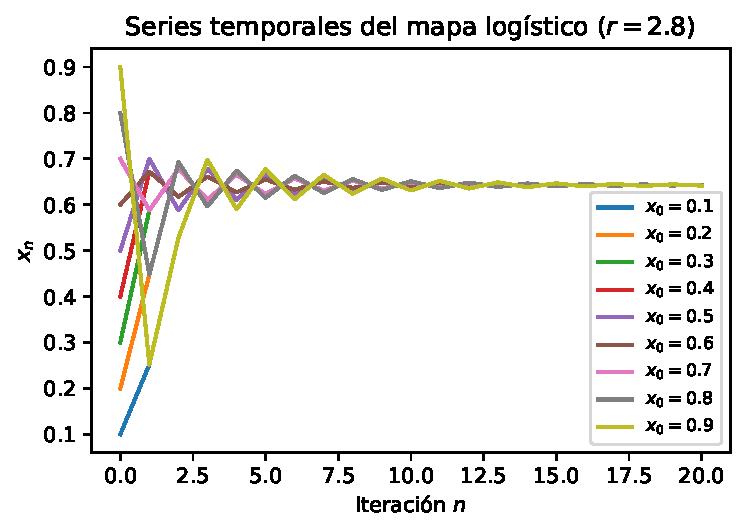
\includegraphics[keepaspectratio]{01-logistica/lyapunov_files/figure-pdf/cell-2-output-1.pdf}}

Y para \(r=3.1\), vemos como también los puntos alcanzados son los
mismos para valores próximos de inicio de la sucesión.

\pandocbounded{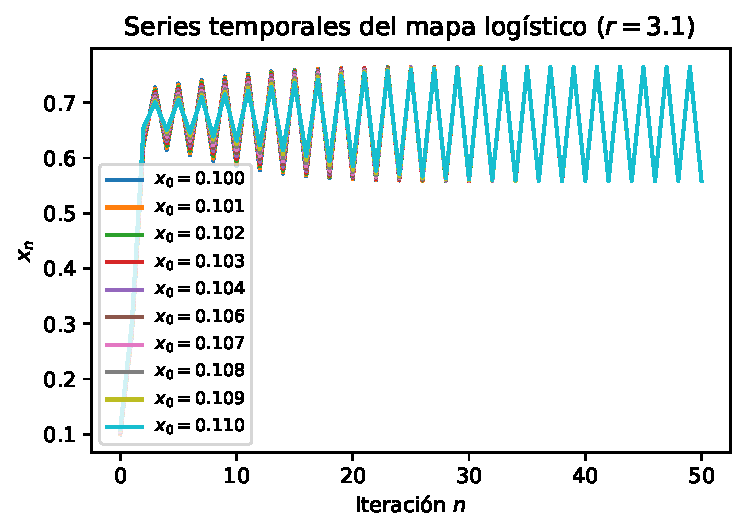
\includegraphics[keepaspectratio]{01-logistica/lyapunov_files/figure-pdf/cell-3-output-1.pdf}}

En los dos casos anteriores, no parece que la evolución del sistema sea
sensible a la condición inicial de partida. Tras unas pocas iteraciones,
da igual de donde se parta, que se converge al mismo punto.

Pero, ¿qué pasa cuando estamos en las zonas caóticas?. Veamos la
iteración del mapa logístico para \(r=3.69\) partiendo de dos valores
muy similares, que solo se separan en \(10^{-5}\) unidades.

\pandocbounded{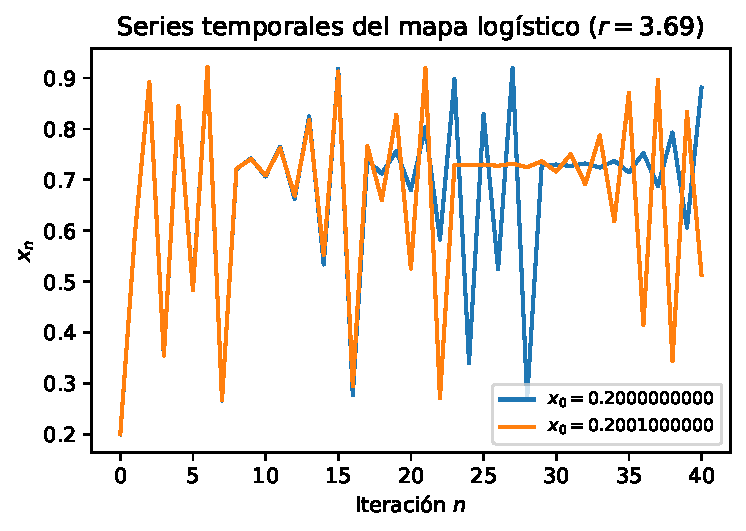
\includegraphics[keepaspectratio]{01-logistica/lyapunov_files/figure-pdf/cell-4-output-1.pdf}}

A la vista del gráfico, vemos como a partir de la iteración 10 empiezan
a haber pequeñas diferencias que se van amplificando a medida que avanza
la simulación. Aquí vemos que sí que empieza a haber sensibilidad a las
condiciones iniciales.

Probemos con una diferencia de valores iniciales aún mas pequeña, en
este caso \(10^{-7}\) unidades.

\pandocbounded{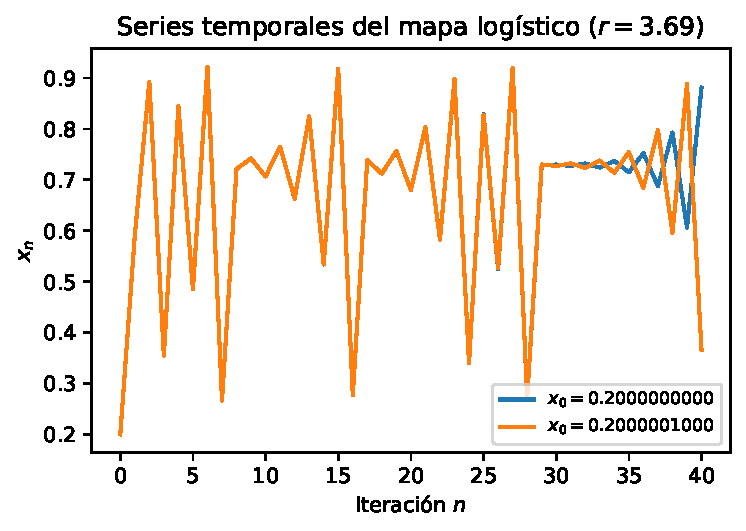
\includegraphics[keepaspectratio]{01-logistica/lyapunov_files/figure-pdf/cell-5-output-1.pdf}}

Ahora la separación de ambas simulaciones se produce a partir de la
iteración número 30. Vamos con una diferencia aún mas pequeña, ahora
\(10^{-10}\) unidades.

\pandocbounded{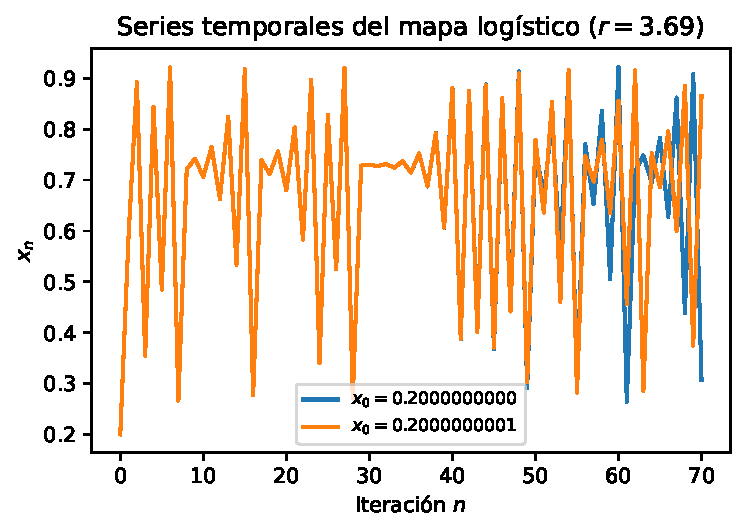
\includegraphics[keepaspectratio]{01-logistica/lyapunov_files/figure-pdf/cell-6-output-1.pdf}}

La separación entre ambas curvas empieza a hacerse visible a partir de
la iteración 50. ¿Qué pasa si hacemos la diferencia aún más pequeña, en
este caso \(10^{-15}\) unidades?. Pues como vemos en la siguiente
gráfica, a partir de la iteración 85 empezamos a ver la divergencia de
ambas sucesiones.

\pandocbounded{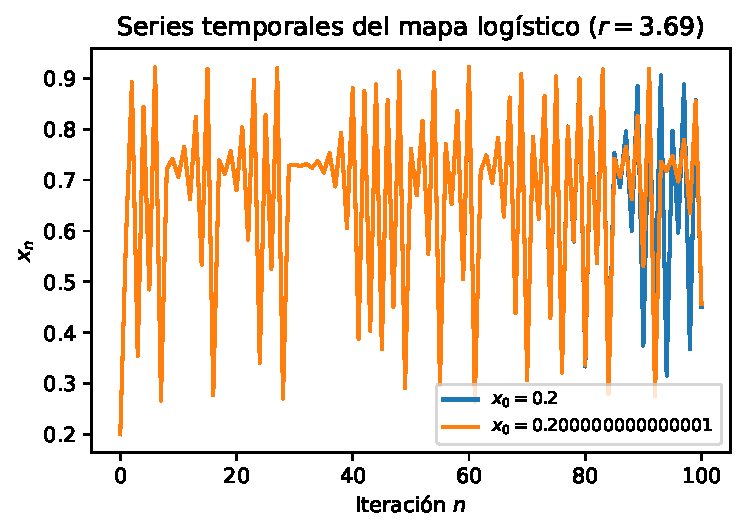
\includegraphics[keepaspectratio]{01-logistica/lyapunov_files/figure-pdf/cell-7-output-1.pdf}}

¿Qué está pasando aquí?. ¿Cómo puede ser que dos valores iniciales que
se diferencian en un valor tan pequeño como \(10^{-15}\) unidades den
valores tan diferentes tras 100 iteraciones?. Si las unidades fueran
metros, estaríamos hablando de una diferencia de un femtómetro. Y aún
más importante: si quiero simular un sistema físico como éste en la
región caótica, ¿cómo voy a poder medir su condición inicial con tal
precisión?. De hecho, parece que la precisión requerida sería infinita.
A poco que me equivoque en la estimación de la condición inicial, no voy
a poder calcular bien su estado final pasado un número grande de
iteraciones. ¿Cómo puede ser si mi sistema es determinista y está regido
por una ecuación tan sencilla?. Hemos topado con el caos y el
\textbf{efecto mariposa}. Y lo inquietante es que este fenómeno se da en
sistemas físicos como la meteorología.

\subsection{Inestabilidad de los cálculos
numéricos}\label{sec-inestabilidad}

Cuando nos encontramos con un sistema físico con alta dependencia a las
condiciones iniciales, no solamente tenemos el problema de conocer con
total exactitud el estado inicial del sistema, sino que como veremos a
continuación los cálculos numéricos que hacemos en nuesto ordenador para
estudiar su evolución se vuelven también muy inestables. A continuación
pondré un ejemplo sobre lo que acabo de decir.

Pongamos que quiero simular el mapa logístico tal cual lo he estado
haciendo en las secciones anteriores. La fórmula es superconocida
(form1):

\[
x_{n+1} = r\,x_n\,(1 - x_n)
\]

Pero también podríamos expresarlo como (form2):

\[
x_{n+1} = r\,x_n - r\,{x_n}^2
\]

Matemáticamente son equivalentes pero a un computador le estamos
diciendo cosas diferentes. * En el primer caso le decimos que reste 1
menos \{x\_n\}, y que a continuación lo multiplique por \(r\) y \(x_n\).
En total 1 resta y dos multiplicaciones * En el segundo caso le decimos
que multiplique por \(r\) y \(x_n\) por un lado. Por otro lado que que
eleve \(x_n\) al cuadrado, y que lo multiplique por \(r\). Y al final
que reste el primer resultado intermedio menos el segundo. En total 1
resta, 2 multiplicaciones y 1 cuadrado.

A esto hay que añadir que en un ordenador los números decimales se
representan mediante aproximaciones. Por ejemplo, con 32 bits,el número
0.2 se representa como 0.200000003, debido a la precisión finita que dan
los 32 bits. Por lo tanto entre el número real y el que representamos,
la mayoría de veces va a haber un error. Estos errores se comportarán de
manera diferente según los cálculos aritméticos que hagamos con ellos.
En el siguiente plot, vemos los errores en un ordenador entre las dos
fórmulas al partir del valor \(x_0=0.2\) y con un \(r=4\).

\pandocbounded{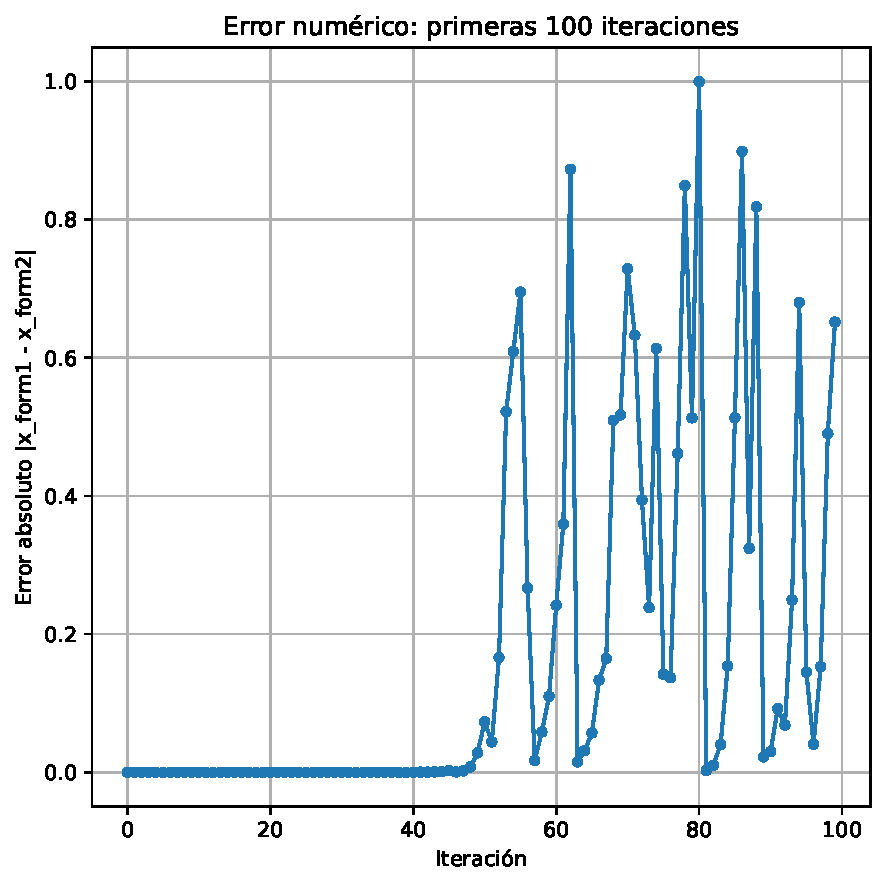
\includegraphics[keepaspectratio]{01-logistica/lyapunov_files/figure-pdf/cell-8-output-1.pdf}}

Vemos como al principio el error es imperceptible, pero a media que
avanzamos va creciendo. A partir de la iteración 50 este error se hace
ya notable, y desde entonces se puede decir que ambas fórmulas
evolucionan de forma totalmente distinta. Por lo tanto, vemos como en un
sistema caótico, no sólo las condiciones iniciales determinan el valor
final de forma extrema, sino que también cuando simulamos este sistema
en una máquina computacional, la forma en la que se representan los
números y la forma de las operaciones también influyen de forma muy
notable.

Pero vamos a ir un paso más. Veamos que evolución tienen realmente los
errores. Para poder bien los errores al principio y al final, vamos a
usar una escala logarítmica en el eje Y. El resultado se muestra a
continuación.

\pandocbounded{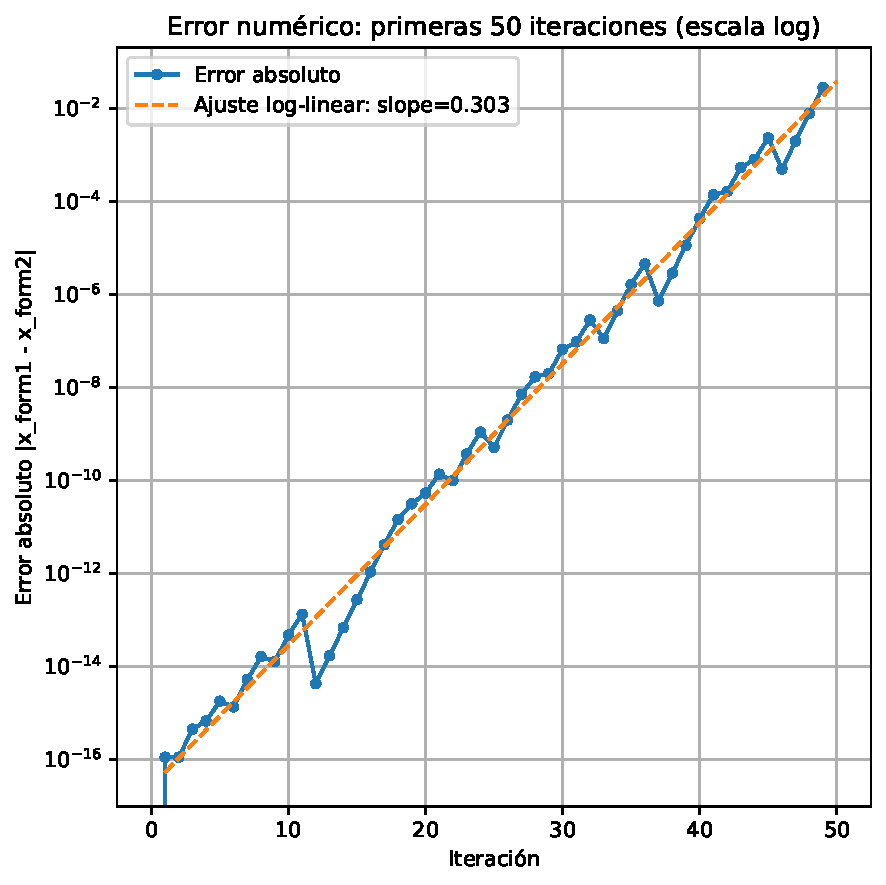
\includegraphics[keepaspectratio]{01-logistica/lyapunov_files/figure-pdf/cell-9-output-1.pdf}}

¿Qué es lo que vemos?. Que los errores crecen linealmente dentro de la
escala logarítmica.

En escala \(\log_{10}\) hemos ajustado: \[
\log_{10}(\mathrm{error}_n)\approx 0.303\,n + C
\] donde \(C\) es la ordenada en el origen. Pasando de logaritmos a
forma explícita: \[
\mathrm{error}_n \approx 10^C \times 10^{0.303\,n}
= A\,\bigl(10^{0.303}\bigr)^n
\approx A\,2^n,
\] puesto que \(10^{0.303}\approx2\).

Equivalentemente, en base \(e\): \[
\ln(\mathrm{error}_n)
= \ln(10)\,\log_{10}(\mathrm{error}_n)
\approx (0.303\,\ln 10)\,n + \ln A
\approx 0.698\,n + \ln A,
\] de donde \[
\mathrm{error}_n \approx A\,e^{0.698\,n}\approx A\,(2.01)^n.
\]

\textbf{Conclusión.} El error crece de forma \textbf{exponencial} con
\(n\), aproximadamente duplicándose en cada iteración.

Curioso, ¿verdad?. El error se va multiplicando por 2 en cada iteración.
Por 2 exactamente. ¿A qué se debe esto????

\section{Cálculo matemático de la amplificación de desviaciones
iniciales}\label{cuxe1lculo-matemuxe1tico-de-la-amplificaciuxf3n-de-desviaciones-iniciales}

A continación daremos una explicación matemática a este fenómeno que
estamos observando.

Imagina que quieres predecir el tiempo atmosférico. Nunca conoces la
temperatura, presión o humedad con absoluta precisión: siempre hay un
error mínimo en la medición. Si ese error crece muy despacio, podrías
predecir con confianza varios días por delante. Pero si crece muy
rápido, tu predicción se vuelve inútil en muy poco tiempo.

En los siguientes párrafos, veros un concepto matemático muy útil en el
estudio del caos: el \textbf{exponente de Lyapunov}, que llamaremos
\(\lambda\) y que cuantifica la tasa de crecimiento de estos errores.

\subsection{Error inicial}\label{error-inicial}

\begin{itemize}
\tightlist
\item
  Sea \(x_0\) el estado ``verdadero'' del sistema en el tiempo
  inicial.\\
\item
  Tu medida real tiene un pequeño error \(\delta_0\), de modo que en
  realidad partes de\\
  \[
     x_0 + \delta_0,
     \quad\text{con}\;|\delta_0|\ll 1.
   \]
\end{itemize}

Ese \(\delta_0\) es tan pequeño que, al principio, los dos estados están
casi juntos. Es lo que hemos visto en los ejemplos anteriores, donde en
la primera iteración las dos simulaciones estaban casi juntas.

\subsection{Cómo evoluciona el error}\label{cuxf3mo-evoluciona-el-error}

Supón que el sistema avanza según una regla \(f\) (nuestra función
logística), es decir: \[
x_{n+1} = f(x_n).
\] Queremos ver qué sucede con \(\delta_n\), la diferencia en el paso
\(n\). Para ello:

\begin{enumerate}
\def\labelenumi{\arabic{enumi}.}
\item
  \textbf{Linealizamos} la función \(f\) alrededor de \(x_n\).\\
  Si \(f\) es suave, podemos aproximar \[
    f(x_n + \delta_n)
    \approx f(x_n)
         + f'(x_n)\,\delta_n,
  \] donde \(f'(x_n)\) es la \textbf{derivada} (o pendiente) de \(f\) en
  \(x_n\).
\item
  De esta aproximación se deduce que \[
    \delta_{n+1} 
    = f(x_n + \delta_n) - f(x_n)
    \approx f'(x_n)\,\delta_n.
  \]
\end{enumerate}

Pero ojo. Cuando calculamos errores, siempre son distancia, es decir
debe ser siempre un número no negativo. La derivada indica pendiente y
sentido.Cuando linealizamos\\
\[
   f(x_n + \delta_n)\approx f(x_n) + f'(x_n)\,\delta_n,
   \]\\
el término \(f'(x_n)\,\delta_n\) nos da \textbf{cuánto} y en \textbf{qué
dirección} cambia la diferencia \(\delta_n\).

La distancia ha de ser siempre no negativa. Por tanto, definimos : \[
   \delta_{n+1} = \bigl|\,x'_{n+1} - x_{n+1}\bigr|.
   \]\\
Sin valor absoluto, un \(f'(x_n)<0\) haría que la ``distancia''
resultase negativa, lo cual no tiene sentido para una medida de error.

El verdadero error en módulo es \(\bigl|f'(x_n)\bigr|\)\$ porque:

\begin{itemize}
\tightlist
\item
  Si \(\lvert f'(x_n)\rvert>1\), la distancia \textbf{aumenta}\\
\item
  Si \(\lvert f'(x_n)\rvert<1\), la distancia \textbf{disminuye}
\end{itemize}

Pongamos un ejemplo numérico: Supongamos \(f'(x_n)=-2\) y
\(\delta_n=0.01\):

\begin{itemize}
\tightlist
\item
  Sin valor absoluto:\\
  \[
  \delta_{n+1}\approx(-2)\times0.01=-0.02\quad(\text{sin sentido físico}).
  \]\\
\item
  Con valor absoluto:\\
  \[
  \delta_{n+1}\approx\bigl|-2\bigr|\times0.01=2\times0.01=0.02,
  \]\\
  reflejando correctamente que la distancia se \textbf{duplica}.
\end{itemize}

Por todo ello, la fórmula adecuada para la evolución del error es\\
\[
\delta_{n+1} \approx \bigl|f'(x_n)\bigr|\,\delta_n,
\]\\
garantizando que \(\delta_{n+1}\ge0\) y midiendo la \textbf{magnitud}
real del estiramiento en cada paso.

\section{Errores sucesivos}\label{errores-sucesivos}

Si repetimos la relaciones anterior paso a paso obtenemos

\begin{enumerate}
\def\labelenumi{\arabic{enumi}.}
\item
  Primera iteración\\
  \[
  \delta_1 \approx \bigl|f'(x_0)\bigr|\,\delta_0.
  \]
\item
  Segunda iteración. En este caso es la derivada en \(x_1\) multiplicado
  por el error anterior (utilizamos para el error anterior la fórmula
  del paso 1). En total vemos que el error en la segunda iteración, es
  el error inicial multiplicado por dos derivadas. \[
  \delta_2
  \approx \bigl|f'(x_1)\bigr|\,\delta_1
  \approx \bigl|f'(x_1)\bigr|\;\bigl|f'(x_0)\bigr|\;\delta_0.
  \]
\item
  Tercera iteración. Aquí ya vemos como aparece un patrón. Vamos
  multiplicando el error inicial por las sucesivas derivadas. \[
  \delta_3
  \approx \bigl|f'(x_2)\bigr|\,\delta_2
  \approx \bigl|f'(x_2)\bigr|\;\bigl|f'(x_1)\bigr|\;\bigl|f'(x_0)\bigr|\;\delta_0.
  \]
\end{enumerate}

En general, para cualquier (n\ge1) podemos generalizar el patrón
encontrado:\\
\[
\delta_n
\;\approx\;
\Bigl(\prod_{k=0}^{n-1}\bigl|f'(x_k)\bigr|\Bigr)\;\delta_0.
\]

\section{De producto a suma}\label{de-producto-a-suma}

Para manejar productos es muy útil usar los logaritmos, porque
transforman productos en sumas: \[
\ln\bigl(\delta_n/\delta_0\bigr)
= \ln\Bigl(\prod_{k=0}^{n-1} f'(x_k)\Bigr)
= \sum_{k=0}^{n-1}\ln\bigl|f'(x_k)\bigr|.
\]

Esta formula nos da el logaritmo de cuánto ha crecido el error tras n
iteraciones en relación al error inicial.

\section{\texorpdfstring{Definición del exponente de Lyapunov
\(\lambda\)}{Definición del exponente de Lyapunov \textbackslash lambda}}\label{definiciuxf3n-del-exponente-de-lyapunov-lambda}

Sabemos según la fórmula anterior, cuánto ha crecido el error en \(n\)
iteraciones. Ahora bien, estaría mejor saber cuanto crece de media por
cada iteración. Para ello, solo tenemos que dividir la suma anterior
entre \(n\).

\[
\frac{1}{n}\,\sum_{k=0}^{n-1}\ln\bigl|f'(x_k)\bigr|.
\]

Ahora vamos a suponer que la simulación es muy larga y que queremos
hacer un promedio. Para ello tomamos el límite cuando \(n\to\infty\) de
la expresión anterior: \[
\lambda
= \lim_{n\to\infty}
\frac{1}{n}\,\sum_{k=0}^{n-1}\ln\bigl|f'(x_k)\bigr|.
\]

Este factor \(\lambda\) es lo que crece de media el error en cada
iteración en mi sistema. LO que crece de forma logarítmica. Lo que crece
realmente en magnitud en cada iteración es \(e^\lambda\)

\begin{itemize}
\tightlist
\item
  Si \(\lambda>0\), el error crece con cada iteracion, puesto que el
  número \(e\) elevado a un valor positivo siempre da un número mayor
  que 1. Puesto que multiplico mi error por un número mayor que 1, el
  error va creciendo iteración tras iteración
  (\(e^\lambda\)\(e^\lambda\)\(e^\lambda\)\ldots\ldots=\((e^\lambda)^n\)=\(a^n\)
  con \(a>1\)) . Crece por lo tanto \textbf{exponencialmente}, y el
  sistema es \textbf{caótico} (muy sensible a la precisión inicial).
\item
  Si \(\lambda<0\), el error \textbf{se atenúa} y las trayectorias
  convergen (sistema estable).La argumentación es justa la contraria del
  caso anterior. El número \(e\) elevado a un valor negativo siempre da
  un número menor que 1.
\item
  Si \(\lambda=0\), estamos en un caso límite de inestabilidad neutra.
\end{itemize}

\section{Cálculo del exponente de Lyapunov para el mapa
logístico}\label{cuxe1lculo-del-exponente-de-lyapunov-para-el-mapa-loguxedstico}

Consideramos el \textbf{mapa logístico}\\
\[
x_{n+1} = f(x_n) = r\,x_n\,(1 - x_n),
\]

La derivada de \(f\), tal y como hemos visto en anteriores secciones,
es\\
\[
f'(x) = r\,(1 - 2x).
\]

Por lo tanto, si tenemos una sucesión de puntos compuesta por
\(x_0, x_1, \dots, x_{N}\), el exponente de Lyapunov máximo se calculará
a partir de la multiplicación de las derivadas de la función logística
en cada uno de los puntos de la sucesión, es decir,

\[
\lambda = \lim_{N\to\infty} \frac{1}{N} \sum_{n=0}^{N-1} \ln\bigl|f'(x_n)\bigr|
        = \lim_{N\to\infty} \frac{1}{N} \sum_{n=0}^{N-1} \ln\bigl|r\,(1 - 2x_n)\bigr|.
\]

En la práctica, no podemos llevar la sucesión al infinito, por lo que
tomamos N iteraciones y aplicamos la siguiente fórmula aproximada

\[
\lambda_N = \frac{1}{N} \sum_{k=0}^{N-1} \ln\bigl|f'(x_k)\bigr|
= \frac{1}{N} \sum_{k=0}^{N-1} \ln\bigl|4\,(1 - 2x_k)\bigr|.
\]\\
Al aumentar \(N\), \(\lambda_N\) tenderá a \(\lambda\).

\subsection{\texorpdfstring{Ejemplo numérico sencillo
(\(N=20\))}{Ejemplo numérico sencillo (N=20)}}\label{sec-exponente}

Vamos a calcular el exponente de Lyapunov para el caso de \(r=4\). Tal y
como vimos en las simulaciones que hicimos en el primer apartado, con
\(r=4\) se prevé que el error se vaya doblando en cada paso, o lo que es
lo mismo, que el exponente de Lyapunov sea
\(\lambda = \ln 2 \approx 0.6931\)

Tomemos de nuevo el mapa logístico con \(r = 4\), es decir, \[
f(x) = 4x(1 - x),
\] y su derivada \[
f'(x) = 4(1 - 2x).
\] Queremos calcular el exponente de Lyapunov aproximado usando \(20\)
iteraciones, empezando con \[
x_{0} = 0.3000
\] Para ello, iremos calculando sucesivamente cada
\(x_{n+1} = f(x_{n})\), el valor absoluto de la derivada
\(\lvert f'(x_{n})\rvert\), y luego \(\ln\lvert f'(x_{n})\rvert\).
Mostraremos en la siguiente tabla \(x_{n}\) redondeado a cuatro cifras
decimales, \(\lvert f'(x_{n})\rvert\) redondeado a cuatro cifras
decimales, y \(\ln\lvert f'(x_{n})\rvert\) redondeado a tres cifras
decimales.

\begin{longtable}[]{@{}
  >{\centering\arraybackslash}p{(\linewidth - 6\tabcolsep) * \real{0.0806}}
  >{\centering\arraybackslash}p{(\linewidth - 6\tabcolsep) * \real{0.1613}}
  >{\centering\arraybackslash}p{(\linewidth - 6\tabcolsep) * \real{0.4677}}
  >{\centering\arraybackslash}p{(\linewidth - 6\tabcolsep) * \real{0.2903}}@{}}
\toprule\noalign{}
\begin{minipage}[b]{\linewidth}\centering
\(n\)
\end{minipage} & \begin{minipage}[b]{\linewidth}\centering
\(x_{n}\)
\end{minipage} & \begin{minipage}[b]{\linewidth}\centering
\(|f'(x_{n})|\)
\end{minipage} & \begin{minipage}[b]{\linewidth}\centering
\(\ln|f'(x_{n})|\)
\end{minipage} \\
\midrule\noalign{}
\endhead
\bottomrule\noalign{}
\endlastfoot
0 & 0.3000 & \(|4(1 - 2\cdot0.3000)| = 1.6000\) & 0.470 \\
1 & 0.8400 & \(|4(1 - 2\cdot0.8400)| = 2.7200\) & 1.001 \\
2 & 0.5376 & \(|4(1 - 2\cdot0.5376)| = 0.3008\) & -1.201 \\
3 & 0.9953 & \(|4(1 - 2\cdot0.9953)| = 3.9548\) & 1.375 \\
4 & 0.0186 & \(|4(1 - 2\cdot0.0186)| = 3.8201\) & 1.340 \\
5 & 0.0879 & \(|4(1 - 2\cdot0.0879)| = 3.2964\) & 1.193 \\
6 & 0.3208 & \(|4(1 - 2\cdot0.3208)| = 1.4332\) & 0.360 \\
7 & 0.8716 & \(|4(1 - 2\cdot0.8716)| = 2.9729\) & 1.090 \\
8 & 0.4476 & \(|4(1 - 2\cdot0.4476)| = 0.4191\) & -0.870 \\
9 & 0.9890 & \(|4(1 - 2\cdot0.9890)| = 3.9122\) & 1.364 \\
10 & 0.0434 & \(|4(1 - 2\cdot0.0434)| = 3.6526\) & 1.295 \\
11 & 0.1661 & \(|4(1 - 2\cdot0.1661)| = 2.6708\) & 0.982 \\
12 & 0.5542 & \(|4(1 - 2\cdot0.5542)| = 0.4333\) & -0.836 \\
13 & 0.9883 & \(|4(1 - 2\cdot0.9883)| = 3.9061\) & 1.363 \\
14 & 0.0464 & \(|4(1 - 2\cdot0.0464)| = 3.6289\) & 1.289 \\
15 & 0.1770 & \(|4(1 - 2\cdot0.1770)| = 2.5844\) & 0.949 \\
16 & 0.5826 & \(|4(1 - 2\cdot0.5826)| = 0.6605\) & -0.415 \\
17 & 0.9727 & \(|4(1 - 2\cdot0.9727)| = 3.7819\) & 1.330 \\
18 & 0.1061 & \(|4(1 - 2\cdot0.1061)| = 3.1512\) & 1.148 \\
19 & 0.3794 & \(|4(1 - 2\cdot0.3794)| = 0.9651\) & -0.036 \\
\end{longtable}

Cada fila se interpreta así:

\begin{enumerate}
\def\labelenumi{\arabic{enumi}.}
\tightlist
\item
  Calculamos \(x_{n+1} = 4\,x_{n}\,(1 - x_{n})\) usando el valor exacto
  de \(x_{n}\) y luego redondeamos el resultado a cuatro decimales para
  mostrarlo.
\item
  Evaluamos la derivada en el valor exacto de \(x_{n}\):
  \(f'(x_{n}) = 4(1 - 2x_{n})\), tomamos su valor absoluto, y lo
  redondeamos a cuatro decimales.
\item
  Finalmente, calculamos \(\ln\lvert f'(x_{n})\rvert\) a partir del
  valor de la derivada ya redondeada, y lo redondeamos a tres decimales.
\end{enumerate}

Ahora sumamos todos los logaritmos obtenidos: \[
\begin{aligned}
\sum_{k=0}^{19} \ln\lvert f'(x_{k})\rvert \;=\;& 
0.470 + 1.001 \;-\; 1.201 + 1.375 + 1.340 + 1.193 + 0.360 + 1.090 \;-\; 0.870 + 1.364 \\
&+ 1.295 + 0.982 \;-\; 0.836 + 1.363 + 1.289 + 0.949 \;-\; 0.415 + 1.330 + 1.148 \;-\; 0.036 \\
=\;& 13.191.
\end{aligned}
\] Por último promediamos esta suma, por lo que el exponente de Lyapunov
aproximado para \(N = 20\) queda como \[
\lambda_{20} 
= \frac{1}{20} \sum_{k=0}^{19} \ln\lvert f'(x_{k})\rvert 
= \frac{13.191}{20} = 0.6596.
\]

Como vemos, el valor \(0.6596\) es muy próximo al teórico \(0.6931\). De
hecho, \(e^{0.6596}=1.934\) que está muy cerca de \(2\).

Para \(N = 20\) hemos obtenido \(\lambda_{20} \approx 0.6596\). Si
continuáramos con más iteraciones, como \(N = 100\) o \(N = 1000\),
veríamos que \(\lambda_{N}\) se acerca gradualmente a \(0.6931\). Esto
muestra que, aunque las primeras iteraciones pueden desviarse, al
promediar sobre muchas iteraciones el resultado converge al
\textbf{valor exacto} del exponente de Lyapunov para \(r = 4\).

\subsection{Cálculo del coeficiente de Lyapunov para todo el mapa
logístico}\label{cuxe1lculo-del-coeficiente-de-lyapunov-para-todo-el-mapa-loguxedstico}

Vamos a aplicar este procedimiento para todos los valores de \(r\) en el
mapa logístico. Y vamos a ser más precisos; para cada valor de \(r\)
haremos 1000 iteraciones en lugar de 20, calcularemos la derivada en
cada uno de los puntos, y sumaremos sus logaritmos. El resultado es el
que se muestra a continuación

\pandocbounded{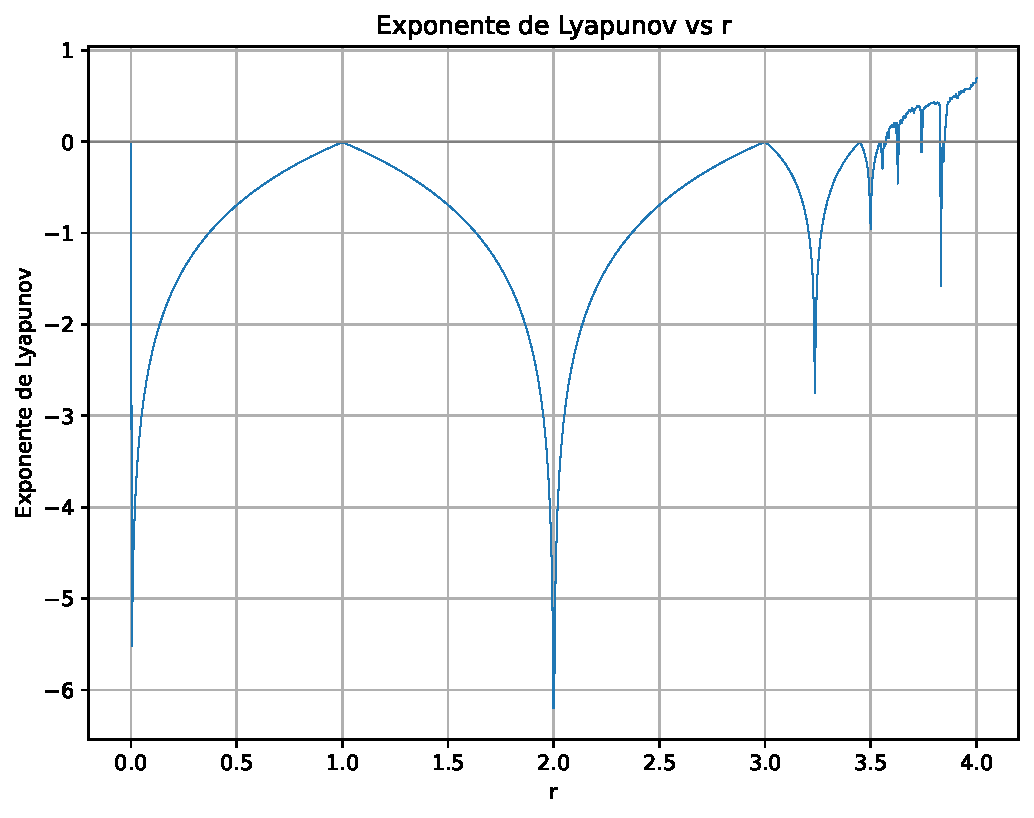
\includegraphics[keepaspectratio]{01-logistica/lyapunov_files/figure-pdf/cell-10-output-1.pdf}}

Vamos a interpretar esta gráfica, y ver si cuadra con los conocimientos
previos del mapa logístico.

Para valores \textbf{\(0 < r \le 1\)}, sabemos que todas las iteraciones
convergen al punto fijo \(x^* = 0\). Por lo tanto el exponente de
Lyapunov: \(\lambda(r) < 0\) ya que no estamos en la zona caótica.

Para \(r = 1\), la ecuación del mapa logístico es \[
   x_{n+1} \;=\; 1 \cdot x_n \,(1 - x_n) \;=\; x_n \,(1 - x_n).
   \]

Los puntos fijos (soluciones de \(x^* = x^*(1 - x^*)\)) se determinan
resolviendo \[
   x^* = x^*(1 - x^*) 
   \quad\Longrightarrow\quad
   x^*(1 - (1 - x^*)) = 0 
   \;\Longrightarrow\;
   x^* \bigl(1 - 1 + x^*\bigr) = 0 
   \;\Longrightarrow\;
   x^* \cdot x^* = 0.
   \]

Por tanto, el único punto fijo es \[
   x^* = 0.
   \]

La derivada del mapa general es \[
   f'(x) = r\,(1 - 2x).
   \]

Si evaluamos en \(r = 1\) en el punto fijo \(x^* = 0\), obtenemos \[
   f'(x^*) \;=\; 1 \cdot \bigl(1 - 2 \cdot 0\bigr) \;=\; 1.
   \]

Es decir, las iteraciones siempre terminan en una derivada igual a 1,
cuyo logaritmos es cero. Por eso el coeficiente de Lyapunov promediado
es cero.

Para valores \textbf{\(1 < r < 3\)}, vemos que de nuevo el exponente es
negativo. En esta zona la función logística tiende a valores estables
comprendidos entre 0 y 1, pero ni es caótica ni periódica. Podemos verlo
matemáticamente, ya que sabemos que en esta zona el mapa logístico
tiende al punto fijo \(1-1/r\), y si evaluamos la derivada de la función
logística en ese punto fijo tenemos \(2 - r\), y como \(1<r<3\) se tiene
\(-1 < 2 - r < 1\), de modo que \(|2 - r|<1\) y por tanto
\(\lambda(r) = \ln|2 - r| < 0\). Es decir, se suman logaritmos que son
siempre negativos, por lo que el promedio final nunca podrá ser
positivo.

Para \(r = 3\) sabemos que el mapa logístico tiende a \[
   x^* \;=\; 1 - \frac{1}{3} \;=\; \frac{2}{3}.
   \]

Evaluándola la derivada en este punto \(x^* = \tfrac{2}{3}\) para
\(r = 3\): \[
   f'\bigl(x^*\bigr) 
   = 3 \cdot \Bigl(1 - 2 \cdot \tfrac{2}{3}\Bigr) 
   = 3 \cdot \Bigl(1 - \tfrac{4}{3}\Bigr) 
   = 3 \cdot \Bigl(-\tfrac{1}{3}\Bigr) 
   = -1.
   \]

Que en valor absoluto es 1, y por lo tanto al igual que el caso con
\(r=1\), el exponente de Lyapunov es cero.

Para \textbf{\(3 < r < r_2 \approx 3.4495\)} sabemos que existe un ciclo
estable de periodo 2. \(\lambda(r)\) en este rango vuelve a ser
negativo, porque aunque ya no convergemos a un punto fijo, sí converge a
un ciclo de periodo 2. En el límite \(r \to r_2\), \(\lambda(r)\) se
acerca nuevamente a 0, pues se produce la segunda bifurcación hacia un
ciclo de periodo 4.

En todos los ciclos restantes hasta \(r_\infty \approx 3.5699456\dots\)*
tenemos el mismo comportamiento, valores negativos en las zonas de los
ciclos y acercandose a cero cuando cambiamos de periodo.

Para \(r_\infty < r \le 4\)** vemos que en la mayoría de estos \(r\) en
los que sabemos que el sistema es caótico se cumple que
\(\lambda(r) > 0\). Sin embargo, dentro de este intervalo caótico
aparecen ``ventanas'' periódicas (por ejemplo, cerca de
\(r\approx 3.8284\), donde hay un ciclo de periodo 3). En esas ventanas
periódicas \(\lambda(r)\) vuelve a ser negativo. Justo en el borde de
cada ventana periódica (bifurcaciones dentro del caos) se tiene
\(\lambda(r)=0\). En la vecindad de \(r = 4\), el valor promedio exacto
es \(\lambda(4) = \ln 2 \approx 0.6931\) tal y como habíamos visto.

\chapter{El exponente de Lyapunov y el
caos}\label{el-exponente-de-lyapunov-y-el-caos}

En la siguiente gráfica vemos lo que hemos ido contanto
pormenorizadamente en la sección anterior. Cada vez que el sistema está
en una zona no caótica, el exponente de Lyapunov es negativo.

\pandocbounded{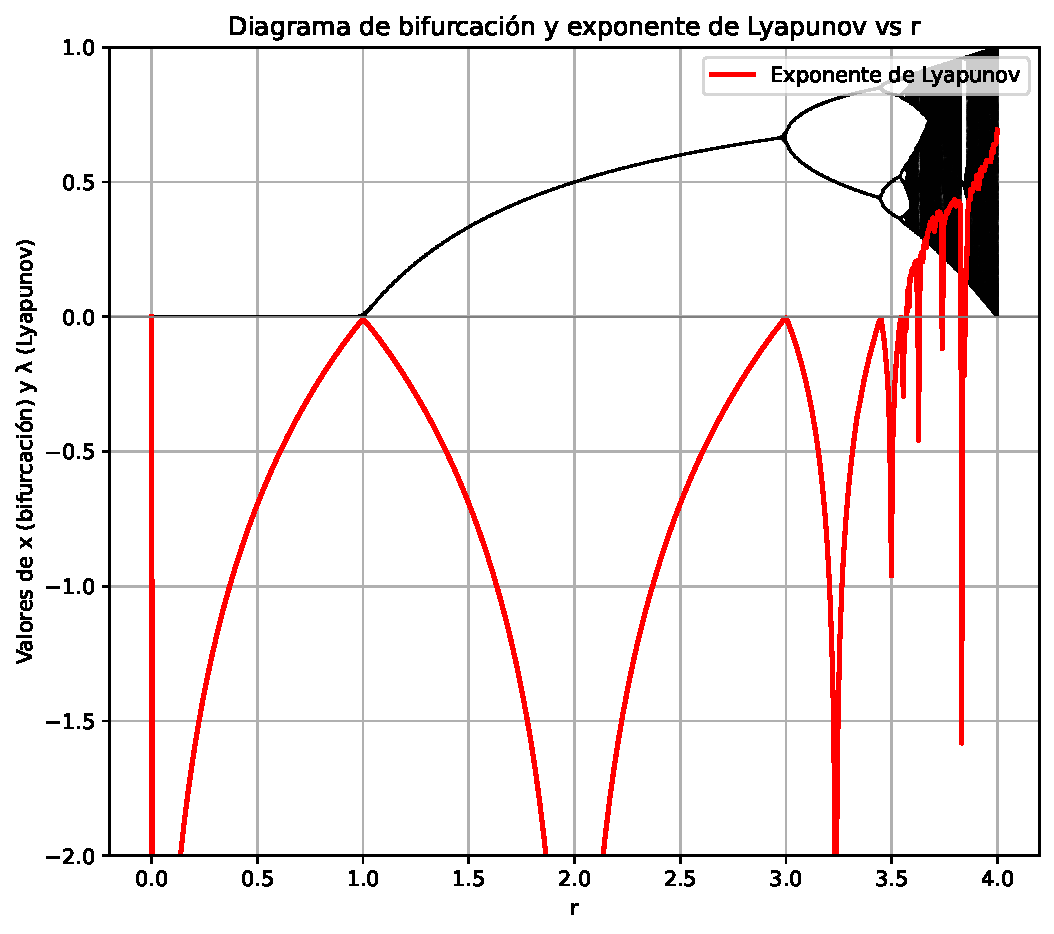
\includegraphics[keepaspectratio]{01-logistica/criterio_files/figure-pdf/cell-2-output-1.pdf}}

De hecho, si hacemos zoom en la zona donde aparece el caos, vemos que en
las ventanas de periodicidad el exponente de Lyapunov se vuelve
negativo.

\pandocbounded{\includegraphics[keepaspectratio]{01-logistica/criterio_files/figure-pdf/cell-3-output-1.pdf}}

La pregunta que debemos hacer es la siguiente, \textbf{¿es el exponente
de lyapunov un indicador que nos puede decir si una serie temporal que
estamos observando es caótica?} Una serie temporal es simplemente una
lista de valores que varían con el tiempo, como por ejemplo la
temperatura diaria de una ciudad: \(T_0, T_1, T_2, \dots\).

Llamamos a esos valores \(x_0, x_1, x_2, \dots\) y cada subíndice indica
la ``etapa'' o ``momento'' en que lo medimos.

Decir que una serie temporal es \textbf{caótica} significa, de acuerdo a
la teoría del caos, que ha de cumplir tres condiciones:

\begin{enumerate}
\def\labelenumi{\arabic{enumi}.}
\tightlist
\item
  \textbf{Es determinista}: existe una ``regla'' (una función) que, dado
  el estado actual \(x_n\), calcula el siguiente \(x_{n+1}\). No hay
  azar puro: si conoces \(x_n\) exactamente, sabes \(x_{n+1}\).\\
\item
  \textbf{Tiene sensibilidad a condiciones iniciales}: dos valores muy
  parecidos \(x_0\) y \(x_0 + \delta_0\) se separan de forma exponencial
  a medida que iteras la regla. Aunque \(\delta_0\) sea minúsculo, al
  cabo de varias iteraciones la diferencia es muy grande.\\
\item
  \textbf{Se ve impredecible a largo plazo}: aunque la regla sea
  determinista, al crecer las diferencias ``desordenadas'' parece un
  comportamiento aleatorio.
\end{enumerate}

Por ejemplo, ir anotando los números que salen directamente de una
ruleta no es una serie caótica, ya que no hay ninguna regla para saber
\(x_{n+1}\) si conoces \(x_n\) exactamente. Eso a pesar de ser
impredecible a largo plazo. Es muy importante hacer notar, que un
sistema caótico tiene unas reglas deterministas muy claras. En este caso
\textbf{no se puede calcular ningún exponente de Lyapunov} porque no hay
función \(f\) continua o diferenciable que escriba \(x_{n+1} = f(x_n)\).
Si intentáramos ``forzar'' un cálculo, estaríamos midiendo ruido y
obtendríamos resultados sin sentido práctico: un ``valor de
\(\lambda\)'' aquí no nos dice nada sobre determinismo o caos, sino solo
sobre la aleatoriedad de los datos.

Otro ejemplo de sistemas que no cumple estas premisas es la bolsa. A
todo el mundo le parece que predecir el valor de una acción a lo largo
del tiempo es muy complejo, pero ¿es caótico?. Para ello veremos como
fuciona la bolsa. El precio de una acción o de un índice bursátil
depende de decenas de variables:\\
• Resultados financieros de las empresas.\\
• Noticias económicas o políticas.\\
• Sentimiento de los inversores y rumores.\\
• Tipos de interés, inflación, datos macroeconómicos.\\
• Eventos inesperados (crisis, pandemias, etc.).

Cada día (o incluso cada minuto) entran al mercado miles de órdenes de
compra y venta, influidas por estas variables.

No existe una regla sencilla \(x_{n+1} = f(x_n)\). A diferencia del mapa
logístico, donde si conocemos \(x_n\) y el parámetro \(r\) podemos
calcular \(x_{n+1} = r\,x_n\,(1 - x_n)\), en la bolsa no hay una función
sencilla y fija que relacione el precio de hoy con el de mañana.

Por estas razones, el precio de la bolsa es, en gran medida, un proceso
aleatorio que incorpora ruido y reacciones humanas, no un sistema
determinista como el mapa logístico.

Volviendo a la pregunta original. \textbf{¿es una condición necesaria y
suficiente para que una serie sea caótica que su exponente de Lyapunov
sea positivo?}

De acuerdo a la investigación bibliográfica realizada, un
\textbf{exponente de Lyapunov mayor} \(\lambda_{\max} > 0\) es
\textbf{condición necesaria} para que un sistema determinista sea
caótico, pero \textbf{no basta por sí solo} para garantizar caos en
sentido completo.

Un sistema se considera \textbf{caótico} si cumple, entre otros, el
criterio de \textbf{sensibilidad a condiciones iniciales}: dos
trayectorias iniciadas en puntos arbitrariamente próximos se separan
exponencialmente con el tiempo. El \textbf{exponente de Lyapunov}
\(\lambda_{\max}\) mide justamente ese crecimiento (o decrecimiento)
exponencial promedio de una pequeña desviación \$ \delta\_0 \$. Si
\(\lambda_{\max} < 0\), todas las pequeñas diferencias se contraen, y el
sistema converge a un punto fijo o a un ciclo periódico estable:
\textbf{no hay caos}. Por lo tanto, \textbf{tener \(\lambda_{\max} > 0\)
es condición necesaria} para hablar de caos determinista

Aunque \(\lambda_{\max} > 0\) garantiza sensibilidad exponencial, para
que un sistema sea considerado caótico \textbf{en el sentido matemático
completo} también se requiere cumplir otras condiciones mas específicas,
que no citaré en este texto por estar muy por encima de mi nivel. La
explicación larga para el lector interesado se haya aquí:

-- ``The short answer is `No'. As reflected in many of the other posted
responses, positive Lyapunov exponents, by themselves, do not always
indicate `chaos'. Additional information about the system \ldots{} needs
to be performed to conclusively diagnose `chaos' in most systems.''\\
Fuente:
\href{https://www.researchgate.net/post/Does-positive-Lyapunov-exponent-always-mean-chaos}{ResearchGate
-- Does positive Lyapunov exponent always mean chaos?}

Sin embargo, en la \textbf{práctica experimental o de series temporales
reales}, suele aceptarse que **si la estimación de \(\lambda_{\max}\)
resulta positiva y se ha verificado que:

\begin{itemize}
\tightlist
\item
  El sistema es determinista (o modelado por un conjunto de ecuaciones
  conocidas).\\
\item
  La variable observada permanece en un rango acotado
\item
  Al simular o analizar la trayectoria, no se observan comportamientos
  puramente periódicos ni divergencias triviales.
\end{itemize}

Entonces, \textbf{la probabilidad de que el sistema sea caótico es muy
alta}. Varios autores y estudios confirman que, bajo condiciones
razonables de ruido controlado, un \textbf{exponente de Lyapunov mayor
positivo} es \textbf{una señal muy confiable de caos determinista}.

-- ``The Largest Lyapunov Exponent (LLE) has been frequently used to
investigate presence of chaotic behavior as well as nonlinear
characteristics of time series.''\\
Fuente:
\href{https://www.sciencedirect.com/topics/engineering/largest-lyapunov-exponent}{ScienceDirect
-- Largest Lyapunov Exponent}

Aunque \textbf{en teoría} hay que cumplir dos condiciones adicionales,
\textbf{en la práctica}, sobre todo en áreas aplicadas (física
experimental, meteorología, etc.), \textbf{una \(\lambda_{\max}\)
positiva suele considerarse como ``casi certeza'' de caos} siempre que
los cálculos se hayan hecho con series suficientemente largas y con
ruido controlado.

\section{Horizonte de
predictibilidad}\label{horizonte-de-predictibilidad}

¿Por qué es tan importante el exponente de Lyapunov al hablar de
sistemas caóticos?. Para ver su importancia vamos a introducir un
término muy importante, el horizonte de predictibilidad.

El \textbf{horizonte de predictibilidad} es el tiempo máximo durante el
cual podemos hacer predicciones fiables de un sistema caótico, dadas
unas condiciones iniciales con cierta incertidumbre. Aunque conozcamos
la regla determinista que rige el sistema, la sensibilidad a las
condiciones iniciales (medida por el exponente de Lyapunov) impone un
límite práctico a nuestra capacidad de predicción.

En un sistema caótico, dos trayectorias que empiezan muy cerca divergen
de forma \textbf{exponencial}. Si la separación inicial entre ellas es
\(\delta_0\), tras un tiempo \(t\) la separación será aproximadamente

\[
\delta(t) = \delta_0\,e^{\lambda_{\max}\,t},
\]

donde \(\lambda_{\max}\) es el \textbf{exponente de Lyapunov máximo},
que mide la rapidez de esa divergencia.

¿Cuándo ``fracasa'' la predicción?

Definimos un \textbf{umbral de error} \(\Delta\): cuando la divergencia
\(\delta(t)\) alcance \(\Delta\), consideramos que la predicción ya no
es útil. Por ejemplo, si medimos temperatura, \(\delta_0\) podría ser la
imprecisión inicial y \(\Delta\) el error máximo tolerable.

Buscamos el tiempo \(T_p\) tal que

\[
\delta(T_p) = \Delta.
\]

Para derivar de la fórmula partimos de\\
\[
   \delta(T_p) = \delta_0\,e^{\lambda_{\max}T_p} = \Delta
   \]

Luego despejamos \(T_p\):\\
\[
   e^{\lambda_{\max}T_p} = \frac{\Delta}{\delta_0}
   \] \[
   \lambda_{\max}T_p = \ln\!\Bigl(\tfrac{\Delta}{\delta_0}\Bigr)
   \] \[
   \boxed{T_p = \frac{1}{\lambda_{\max}}\,\ln\!\Bigl(\tfrac{\Delta}{\delta_0}\Bigr)}
   \]

¿Cuál es el significado de cada término?

\begin{itemize}
\tightlist
\item
  \textbf{\(\lambda_{\max}\)}: mayor exponente → predicciones válidas
  por menos tiempo.\\
\item
  \textbf{\(\delta_0\)}: si reducimos la imprecisión inicial, alargamos
  \(T_p\).\\
\item
  \textbf{\(\Delta\)}: cuanto más tolerante seas al error, más tiempo
  «aguanta» la predicción.
\item
  Un sistema con \(\lambda_{\max}<0\) tendría, en cambio, un horizonte
  de predictibilidad infinito, pues los errores se contraen y la
  predicción mejora con el tiempo.
\end{itemize}

\textbf{Ejemplo práctico:}\\
En la atmósfera se observa a menudo un exponente\\
\[
\lambda_{\max} \approx 0{,}8\ \text{día}^{-1}.
\]

Además, la \textbf{incertidumbre inicial} realista en modelos y medidas
es más alta, por ejemplo\\
\[
\delta_0 = 10^{-3}\ \text{(°C)},
\]\\
y mantenemos el \textbf{error tolerable}\\
\[
\Delta = 1\ \text{°C}.
\]

Entonces,

\[
T_p
= \frac{1}{0.8}\,\ln\!\Bigl(\tfrac{1}{10^{-3}}\Bigr)
=1{,}25 \times \ln(10^3)
=1{,}25 \times 6{,}91
\approx 8{,}6\ \text{días}.
\]

Este cálculo \textbf{coincide} con el límite práctico de \textbf{7--10
días} que vemos hoy en los pronósticos meteorológicos fiables. El lector
puede echar un vistazo al siguiente artículo:

https://www.stratumfive.com/climate/weather-forecasting-and-chaos-theory/

Aquí se habla de un horizonte de predictibilidad para el tiempo de 8 a
10 días. La cuestión es que por lo aprendido en este proyecto, éste
límite es una barrera que no vamos a poder superar. Si bien en los
últimos 50 años se ha producido un formidable incremento de la precisión
con la que hacemos las predicciones, pasando de predicciones fiables a
un día a tener buenas predicciones a 5 días, el llegar a batir este
límite dos semanas va a ser imposible.

Y hablando de horizontes de predictibilidad, ¿qué te parece el escuchar
que el sistema solar tiene un horizonte de prectibilidad de unos 5
millones de años?. Si Newton levantase la cabeza. Es decir, a pesar de
que tenemos esa preciosa fórmula de la gravitación universal, que
funciona tan bien, su propagación hacia el futuro, cuando tenemos en
cuenta los planetas que componen el sistema solar, deja de ser válida a
4 millones de años vista, que en términos cósmicos es poco tiempo. Y es
que no solamente tenemos errores iniciales, al no poder tener en cuenta
todos los pequeños objetos que vagan por el sistema solar, sino porque
el sistema es inherentemente caótico. De hecho, tal y como anticipó
Poincare, el movimiento de tres cuerpos en el vacío sujetos a sus
respectivas fuerzas de atracción gravitatoria, es ya un sistema caótico,
y que presenta un exponente de Lyapunov positivo en determinadas
circustancias.

\subsection{Referencias principales}\label{referencias-principales}

\begin{enumerate}
\def\labelenumi{\arabic{enumi}.}
\tightlist
\item
  Wikipedia. ``Chaos theory.''\\
  \url{https://en.wikipedia.org/wiki/Chaos_theory}\strut \\
\item
  ResearchGate. ``Does positive Lyapunov exponent always mean chaos?''\\
  \url{https://www.researchgate.net/post/Does-positive-Lyapunov-exponent-always-mean-chaos}\strut \\
\item
  Wikipedia. ``Butterfly effect.''\\
  \url{https://en.wikipedia.org/wiki/Butterfly_effect}\strut \\
\item
  ScienceDirect Topics. ``Largest Lyapunov Exponent.''\\
  \url{https://www.sciencedirect.com/topics/engineering/largest-lyapunov-exponent}
\end{enumerate}

\part{El Caos en vivo: El péndulo doble}

\chapter{El Péndulo Doble}\label{el-puxe9ndulo-doble}

\section{Introducción}\label{introducciuxf3n-3}

El péndulo doble es quizás uno de los sistemas físicos más estudiados en
el ámbito de la teoría del caos. Esto es debido a que tiene unas
ecuaciones deterministas muy bien conocidas, y a la contraposición con
el péndulo simple. Es decir, mientras que en el péndulo simple con unas
ecuaciones relativamente más sencillas podemos predecir ``ad infinitum''
la posición y velocidad del péndulo, en el caso del péndulo doble, que
no son más que dos péndulos sencillos acoplados, no podemos predecir más
allá de unos pocos segundos.

Dicho de otra manera, un péndulo simple, como el que estudió Galileo, es
un sistema que encaja perfectamente en la mecánica clásica y que se
comportanta de una forma determinisita, mientras que un pendulo doble
tiene un comportamiento imposible de predecir tras unos pocos segundos.
Ambos están regidos por las mismas leyes de la física, y el péndulo
doble es ligeramente más complejo, pero su comportamiento es totalmente
impredecible. Todo ello a pesar de tener unas ecuaciones que describen a
la perfección su comportamiento.

El análisis matemático de ambos sistemas, el pendulo simple y doble, se
puede obtener en muchas referencias, por ejemplo en
\url{https://paginaspersonales.unam.mx/app/webroot/files/4554/Publica_20190605182303.pdf}.
El análisis matemático del péndulo doble está muy por encima del nivel
de bachillerato.

Sin embargo podemos recurrir a la simulación y experimentación real para
analizar su comportamiento. Empezaremos por realizar simulaciones y
comprobar en el ordenador como se comporta el pendulo doble. Pero, ¿no
resulta muy complicado hacer la simulación de un péndulo doble?. ¿Acaso
no habría que implementar las ecuaciones del pendulo doble, que resultan
realmente complicadas de analizar matemáticamente?. Tenemos dos
soluciones para ello:

\begin{itemize}
\tightlist
\item
  Podemos utilizar simuladores de física como Algodoo
  \url{https://www.algodoo.com/}
\item
  Podemos pedirle a ChatGPT que nos haga una simulación en Python.
\end{itemize}

En este proyecto, he optado por la segunda alternativa, y los resultados
han sido espectaculares. Usando uno de los modelos más avanzados de
OpenAI, el mini4-high, la códificación resultó directa y sin errores.
Copiando el código generado, y ejecutándolo desde mi ordenador pude
tener en unos pocos minutos

\chapter{Sensibilidad a las condiciones
iniciales}\label{sensibilidad-a-las-condiciones-iniciales}

\textbf{Autor:} Rubén Torre Merino

\begin{center}\rule{0.5\linewidth}{0.5pt}\end{center}

\section{Descripción General}\label{descripciuxf3n-general}

En esta entrada se analiza un programa escrito en Python para simular y
dibujar \(10.000\) péndulos dobles simultáneamente. El objetivo
principal de la simulación es mostrar la \textbf{sensibilidad a las
condiciones iniciales}, un rasgo característico de los sistemas
caóticos. Cada péndulo comienza con un ángulo inicial ligeramente
distinto para ilustrar cómo pequeñas variaciones pueden dar lugar a
comportamientos muy diferentes a lo largo del tiempo. Es decir, como
verás en el próximo vídeo los péndulos al ser lanzados paracen estar
todos en la misma posición pero a medida que vamos avanzando en la
simulación se separan totalmente.

Figura 1: Esquema del doble péndulo

\begin{center}\rule{0.5\linewidth}{0.5pt}\end{center}

\section{Preparación del Código con
ChatGPT}\label{preparaciuxf3n-del-cuxf3digo-con-chatgpt}

Este código fue \textbf{generado mediante ChatGPT}, aprovechando la
capacidad del sistema para programar en Python. A continuación, se
describe el \emph{prompt} que dio origen a esta simulación:

\begin{quote}
\textbf{Prompt sugerido:}\\
``Genera un código en Python que utilice Python para simular \(10000\)
péndulos dobles al mismo tiempo. Cada péndulo debe tener la primera pata
en la misma posición (170 grados) y la segunda pata con un ángulo
inicial también de 170 grados pero ligeramente distinto en cada péndulo,
espaciado uniformemente entre 170 y 170.1 grados. El objetivo es
visualizar la sensibilidad a las condiciones iniciales superponiendo
todos los péndulos en una misma imagen. Dibuja cada péndulo de un color,
y muestra la animación en tiempo real. Mi ordenador dispone de una
tarjeta gráfica Nvidia y tengo instalado CUDA, así que úsalo para
acelerar las simulaciones. No tengas en cuenta la fuerza de
rozamiento.''
\end{quote}

Tras varias iteraciones de este prompt, al final conseguí un código que
se ejecutase. La depuración del código es realemnte fácil de hacer. Cada
vez que ChatGPT me daba un código, lo corría en el ordenador mediante el
comando ``python programa.py'', y los errores se los alimentaba de
vuelta al ordenador que a su vez me devolvía el código depurado.

En el código proporcionado, los parámetros físicos de cada péndulo doble
los ha definido ChatGPT de la siguiente manera:

\begin{itemize}
\item
  \textbf{Longitudes de los brazos}

  \begin{itemize}
  \tightlist
  \item
    Longitud del primer brazo: \(l_1 = 1.0\) metros\\
  \item
    Longitud del segundo brazo: \(l_2 = 1.0\) metros
  \end{itemize}

  En la representación gráfica cada metro es representado a través de
  150 píxeles.
\item
  \textbf{Masas de los cuerpos}

  \begin{itemize}
  \tightlist
  \item
    Masa del primer cuerpo: \(m_1 = 1.0\) Kg
  \item
    Masa del segundo cuerpo: \(m_2 = 1.0\) Kg
  \end{itemize}

  La gravedad es la terrestre, \(9.81 Kg/m^2\). El péndulo simulado es
  grande, pero lo bueno de hacerlo grande es que va mas lento en tiempo
  que un péndulo pequeño, por lo que su movimiento se aprecia mejor en
  la simulación. El péndulo oscila sin parar ya que no hemos puesto
  ninguna fuerza de rozamiento.
\end{itemize}

\section{Video con la simulación}\label{sec-abanico}

Una vez preparado el código procedía a correrlo y grabar la ventana de
salida en un archivo de vídeo que se encuentra a continuación. Hay que
tener en cuenta que el código Python generado por ChatGPT, avanza en
pasos de 1 milisegundo de tiempo real, y que debido a la gran cantidad
de pendulos la simulación no llega a ser en tiempo real. Por eso le
pedía a ChatGPT que incluyera un texto en la simulación que mostrase el
tiempo real durante la simulación.

El resultado es sorprendente e hipnotizante. ¿Como puede ser que
péndulos que se lanzan tan cercanos diverjan tan rápidamente?. Si
observamos antentamente el vídeo hasta el segundo 1 de la simulación
todos los péndulos van casi al unísono. En el segundo 2, que es cuando
llegan al otro extremo, vemos que el ``abanico'' ya se empieza a abrir.
Y en la bajada que le sigue se desata el caos. Del segundo 2 al tres ya
estamos con una divergencia total, y a partir de ahí cada uno va a su
bola, !!caos total!!.

Ahora reflexionemos. Péndulos que fueron lanzados con diferencias de
milésimas de grado, tienen trayectorias que divergen enormemente tras 5
segundos. ¿Acaso es éste un sistema físico que cuyo comportamiento
podamos predecir en la vida real?. Pues yo diría que no.

\section{Complemento y Reflexiones}\label{complemento-y-reflexiones}

¡Imagínate! Iniciamos todos los péndulos casi de la misma manera, apenas
una pequeña de diferencia en el segundo ángulo. Y, sin embargo, a los
pocos segundos, el espectáculo visual es un torbellino de colores y
líneas que ya no parecen corresponderse entre sí. Fíjate bien: el lector
no ve cinco segundos, sino un universo paralelo donde cada péndulo tiene
su propia historia, su propio destino. ¿Te das cuenta de lo
desconcertante que es?

\subsection{La Belleza del Caos}\label{la-belleza-del-caos}

Tal vez te preguntes: ``¿Por qué es tan atractivo ver este desorden?''.
La respuesta está en la misma naturaleza de lo impredecible. Cada línea
coloreada que se dispersa representa un pequeño ``qué pasaría
si\ldots{}'': un escenario distinto construido por una diferencia
diminuta en los ángulos iniciales. Cuando miras el vídeo, lo que parece
arte abstracto en movimiento es, en realidad, la materialización
instantánea de un principio matemático: el caos.

\subsection{Reflexión sobre la
Predictibilidad}\label{reflexiuxf3n-sobre-la-predictibilidad}

¿Recuerdas cuando en clases nos decían que la física clásica era
determinista? Aquí tenemos una bofetada directa a esa idea: sí, las
ecuaciones son exactas y puntuales, pero cualquier medición en la
realidad lleva error, desviaciones, incertidumbre. Esas milésimas de
grado que apenas vemos en el vídeo se traducen en divergencias drásticas
en segundos. Entonces debes preguntarte:\\
- ¿Podríamos predecir con exactitud el comportamiento de un péndulo real
si midiera su ángulo con la precisión de un nanómetro?\\
- ¿Sería suficiente?

La respuesta es que, por muy maravillosa que sea nuestra
instrumentación, siempre habrá imperfecciones. Ese desajuste, ese ruido
minúsculo, es suficiente para que la simulación sea un recordatorio de
que el mundo real---y nuestros modelos---tienen un límite de
predictibilidad. No solo eso, como vimos en el capítulo anterior con la
función logística, los modelos matemáticos se codifican en un ordenador
con una precisión finita, que a su vez introduce errores iteración tras
iteración de nuestro código. Por lo tanto, nos enfrentamos a dos
problemas en la realidad:

\begin{itemize}
\tightlist
\item
  No podemos medir con total exactitud el estado inicial de nuestro
  sistema
\item
  No podemos simular los modelos matemáticos con una precisión infinita
  en un ordenador
\end{itemize}

\subsection{¿Qué Aprendemos como
Observadores?}\label{quuxe9-aprendemos-como-observadores}

En este punto, quiero que te sientas más que un simple espectador;
quiero que te cuestiones tu propia confianza en la previsión de sistemas
aparentemente simples. Porque, al fin y al cabo, el péndulo doble no es
más que un ejemplo fácil de visualizar, pero el universo real está lleno
de sistemas caóticos: el clima, la dinámica de poblaciones, incluso
ciertos procesos en la economía. Si un experimento tan básico como el
péndulo doble nos muestra esta fragilidad, ¿cómo imaginamos predecir con
total certeza fenómenos tan complejos?

\subsection{Reflexión Final: Una Invitación al
Asombro}\label{reflexiuxf3n-final-una-invitaciuxf3n-al-asombro}

Te invito a que, la próxima vez que veas un pronóstico meteorológico o
leas sobre el futuro de los mercados, recuerdes este vídeo de los
péndulos. Observa cómo cambia cada línea, cómo el abanico se abre a
partir de una diferencia insignificante. Tal vez entonces comprendas que
la exploración del caos no es un simple juego visual, sino un
recordatorio profundo: hay límites invisibles en nuestra capacidad de
anticipar el futuro.

\chapter{Mapa de Fases}\label{mapa-de-fases}

Recordemos que durante el estudio de la función logística, el diagrama
de bifurcación aparecía una y otra vez cada vez que hacíamos zoom en una
zona pequeña de \(r\). Veíamos la misma estructura repetida en zonas de
\(r\) cada vez más pequeñas. ¿Pasará algo similar con el péndulo doble?.
Vamos a ir paso a paso.

En primer lugar vamos a simular 36 x 36 péndulos, cada uno de ellos con
diferentes condiciones iniciales de los dos brazos. Puesto que cada uno
de los ángulos puede tomar 360 grados, vamos a repartirlos en 36
posiciones diferentes cada uno de ellos desde 0,10,20 .. hasta 350
grados. Obviamente, aquí están separados bastante por lo que su
evolución va a ser diferente.

Por lo tanto estamos viendo 1296 péndulos dobles al mismo tiempo! Cada
uno en su pequeña celda de 20×20 píxeles, todos organizados en una
cuadrícula de 36×36. El resultado es una imagen de 720×720 donde cada
cuadradito muestra un péndulo doble distinto, lanzado con ángulos
iniciales que varían sistemáticamente en filas y columnas.

Cada celda se trata como un único péndulo doble, con los mismos
parámetros que en el caso del abanico de péndulos (masas \(m_1=m_2=1\),
longitudes \(l_1=l_2=1\), gravedad \(g=9.81\)).

Se dibujan las líneas de los brazos en blanco y los tres puntos de unión
en colores rojo, verde y azul para los pivotes, la primera masa y la
segunda masa respectivamente.

Con cada iteración, la simulación avanza y se pinta el estado
actualizado, de modo que se ve un baile de péndulos distintos en cada
casilla.

\section{Prompt para Generar Este Script con
ChatGPT}\label{prompt-para-generar-este-script-con-chatgpt}

\begin{quote}
\textbf{Prompt para la generación del código}\\
``Quiero un código en Python para mi tarjeta Nvidia y Cuda para simular
una \textbf{cuadrícula 36×36 de péndulos dobles} en paralelo. Cada celda
debe inicializar su péndulo con un ángulo para el primer brazo
comprendido entre 0 y 350 grados en pasos de 10 grados, y con un ángulo
para el segundo brazo comprendido entre 0 y 350 grados en pasos de 10
grados. Utiliza los siguientes parámetros de simulación para los
péndulos (\(m_1 = m_2 = 1\), \(l_1 = l_2 = 1\), \(g = 9.81\) y cero
rozamiento).\\
Dibuja cada péndulo en su propia celda de 20×20 píxeles dentro de una
imagen global de 720×720. Dibuja los brazos (longitudes 6 píxeles) en
blanco y los pivotes como círculos pequeños en rojo, verde y azul.
Muestra la ventana en tiempo real y sal al presionar Esc.''
\end{quote}

Al ver la cuadrícula completa, el lector observa cómo cambia el
comportamiento del péndulo doble al variar sus ángulos iniciales en
pequeños pasos de 10°. En la esquina superior izquierda
\((-180^\circ,-180^\circ)\) el movimiento puede ser muy distinto al de
la esquina inferior derecha \((+170^\circ,+170^\circ)\).

Es un ``mapa de fase'' visual: cada casilla revela un patrón dinámico
único, mostrando cómo la mecánica no lineal responde a distintos puntos
de partida. ¿Por qué se llama mapa de fase?. Cuando dibujamos una
función senoidal a lo largo del tiempo, vemos un patrón repetido. Si
pintamos otro seno al lado, con igual amplitud y frecuencia, pero
cambiando el ángulo inicial, veremos el mismo patrón pero desplazado en
el tiempo por ese ángulo incial. Estamos por lo tanto en otra ``fase''
del mismo sistema. Otra forma más cotidiana de verlo es con la Luna:
hablamos de fases para referirnos a la iluminación relativa de la Luna
por el Sol tal y como lo vemos desde la Tierra. Así tenemos fase
creciente, menguante, llena, etc.

Vemos una zona central en la que los péndulos parten de ángulos
pequeños. En este caso observamos que el comportamiento es muy similar
al de un péndulo simple. Es, por así decirlo, una zona de estabilidad
del sistema. Pregunté a ChatGPT por qué se produce esta zona de
estabilidad y su respuesta fue la siguiente.

\subsection{Aproximación de Ángulo
Pequeño}\label{aproximaciuxf3n-de-uxe1ngulo-pequeuxf1o}

En la simulación del péndulo doble, cada péndulo tiene dos ángulos
\(\theta_1\) y \(\theta_2\). Cuando ambos son pequeños, la dinámica se
``desacopla'' casi como si fueran dos péndulos simples en serie, pero
sin generar las fuertes interacciones que provocan el caos. Veamos por
qué:

\begin{enumerate}
\def\labelenumi{\arabic{enumi}.}
\tightlist
\item
  Las ecuaciones originales del péndulo doble incluyen términos no
  lineales muy potentes (producto de \(\sin(\theta_1 - 2\,\theta_2)\),
  \(\cos(2\,\delta)\), etc.).\\
\item
  Si \(\theta_1\) y \(\theta_2\) permanecen pequeños, esos términos no
  lineales pierden relevancia: \(\sin(\theta_1)\approx \theta_1\),
  \(\sin(\theta_1 - 2\,\theta_2)\approx \theta_1 - 2\,\theta_2\), y
  \(\cos(2\,\delta)\approx 1\).\\
\item
  Resultado: el sistema casi se comporta como dos péndulos simples que
  oscilan suavemente y de forma \textbf{aproximadamente periódica}. No
  hay ``explosión'' de sensibilidad porque las variaciones pequeñas no
  se amplifican de forma exponencial. Es la zona donde la energía no
  alcanza para explorar el caos.
\end{enumerate}

En otras palabras, en el centro de la ``cuadrícula de fase'' hay un área
donde las trayectorias son estables, casi previsibles, iguales a las que
obtendrías si estudiaras un péndulo simple (o dos acoplados muy
débilmente). Observas oscilaciones regulares, de ida y vuelta, sin
divergencias drásticas.

\subsection{¿Por Qué Llamarlo ``Zona de
Estabilidad''?}\label{por-quuxe9-llamarlo-zona-de-estabilidad}

Cuando hablamos de sistemas dinámicos, llamamos ``estable'' a aquella
región donde las pequeñas perturbaciones no se magnifican con el tiempo.

Si en el experimento gráfico seleccionas solo las celdas centrales,
notarás que los péndulos dobles describen curvas suaves, casi
sinusoidales, muy parecidas a las de un péndulo simple. Esa cohesión de
trayectorias es lo que define la estabilidad: todas las simulaciones de
esa región inicial ``viajan juntas'', sin dispersarse.

\section{Transición hacia el Caos}\label{transiciuxf3n-hacia-el-caos}

A medida que nos alejamos del centro (es decir, cuando comienzas a dar a
\(\theta_1\) o \(\theta_2\) valores más grandes, digamos 30°, 40° o
más), las ecuaciones no lineales cobran protagonismo. Entonces:

\begin{enumerate}
\def\labelenumi{\arabic{enumi}.}
\tightlist
\item
  Los términos \(\sin(\theta)\) ya no son equivalentes a \(\theta\).\\
\item
  Aparecen resonancias internas: la interacción entre el primer y el
  segundo brazo se hace más intensa.\\
\item
  Surge la \textbf{sensibilidad exponencial}: dos péndulos con
  diferencias iniciales de solo unos grados comienzan a divergir
  rápidamente tras pocas oscilaciones.
\end{enumerate}

Así, justo en el borde de esa zona estable, empieza a nacer el caos: las
trayectorias dejan de ser regulares y adquieren formas impredecibles.

Esto nos recuerda a lo que pasaba con la función logística a medida que
crecía \(r\). Hasta \(r=3\) estábamos en una zona muy estable, con un
solo valor final. Ahora el parámetro que controla la estabilidad es el
ángulo desde el que lanzamos el péndulo. Para ángulos pequeños estamos
en zona estable y para ángulos mayores estamos en zonas de caos. En
ambos casos, cuando suministramos más ``energía'' al sistema bien sea en
forma de un mayor \(r\) o un mayor ángulo inicial el sistema se vuelve
caótico.

\section{Mapa de fase detallado}\label{mapa-de-fase-detallado}

Ahora vamos a simular muchísimos más pendulos, para obtener un mapa de
fase mas detallado. Para ello ahora la simulación se organiza en una
cuadrícula de \(720 \times 720\) péndulos. Cada columna \(i\)
corresponde a un ángulo inicial \[
\theta_1(i) \;=\; -\pi \;+\; i\,\frac{2\pi}{719}, 
\quad i = 0,1,\dots,719,
\] y cada fila \(j\) a un ángulo inicial \[
\theta_2(j) \;=\; -\pi \;+\; j\,\frac{2\pi}{719}, 
\quad j = 0,1,\dots,719.
\]

Así, la celda \((i,j)\) arranca con condiciones \[
\theta_1 = \theta_1(i), 
\qquad
\theta_2 = \theta_2(j).
\]

Como cada péndulo es ahora un pixel, ¿cómo podemos visualizar su
estado?. Pues recurrimos a un código de colores. Entonces para cada
péndulo cogemos los angulos \(\theta_1\) y \(\theta_2\) en los que se
encuentra y hacemos una primera normalización. Para cada péndulo se
calculan \[
     n_1 = \frac{\sin(\theta_1) + 1}{2},
     \quad
     n_2 = \frac{\sin(\theta_2) + 1}{2},
   \] de modo que \(n_1,n_2 \in [0,1]\). De esta manera no tenemos
valores negativos del estado, es decir su estado va desde 0 hasta 1.

A continuación promediamos, ambos valores \(n_1\) y \(n_2\) y escalamos
al equivalente de 8 bits, es decir 256 valores, \([0,255]\): \[
     \text{Promedio} = \Bigl(\frac{n_1 + n_2}{2}\Bigr)\times 255.
   \]

Y por último el código generado por ChatGPT aplica un código de colores
al valor promedio resultando en:

azul para valores bajos (\(\approx 0\)),

verde/amarillo para valores intermedios,

rojo para valores altos (\(\approx 255\)).

El resultado de la simulación se puede ver en el siguiente vídeo.

Como anticipabamos en la zona central hay estabilidad, y fuera de ella
no se ven patrones, sino que aparece una especie de ruido. En estas
zonas ``ruidosas'' lo que tenemos es caos, es decir, el estado del
péndulo varía continuamente, y lo que es más importante el estado de
cada péndulo es totalmente distinto de los péndulos vecinos, lo que
manifiesta de nuevo la extrema sensibilidad a las condiciones iniciales.

Para ver más detalladamente esta sensibilidad a las condiciones
iniciales vamos a hacer zooms en areas alejadas del centro. Se hacen
hasta tres zooms consecutivos hasta llegar a una zona rectangular de
0.01 grados x 0.01 grados en las que se simulan los 720x720 péndulos. No
importa cuanto nos adentramos en el mapa de fase: no se consigue que los
péndulos vecinos vayan a la vez

En el siguiente video aparece la misma simulación pero esta vez dejando
que corra más el tiempo. En ella se ve que a medida que avanza la
simulación la zona central se va reduciendo, y el caos se apodera de más
zonas. Hay que tener en cuenta que estamos en un sistema sin rozamiento,
y que puede estar corriendo infinitamente. Zonas que al principio
parecían estables, se convierten en caóticas, quedando una pequeña
porción como estable.

Se pueden ver aparcer algunas pequeñas ``islas'' de estabilidad. Hagamos
en una de ellas y veamos como avanza la simulación en ella:

Al igual que en el caso del mapa logístico hay pequeñas zonas de
estabilidad alejadas del centro, rodeadas de caos. Pero la verdad es que
hay que decir que son unos pocos y limitados casos.

\chapter{Bifurcaciones}\label{bifurcaciones}

¿Qué mas paralelismos podemos encontrar en el doble péndulo al
compararlo con el mapa logístico?. Vamos a hacer un nuevo ejercicio. En
este caso vamos a simular la diagonal del mapa de fases anterior, es
decir, vamos a coger los valores de \(\theta_1\) y de \$\theta\_2\& y
los vamos a variar desde -180 hasta 180 grados simultáneamente por medio
de una sola variable de control. Puesto que el péndulo doble no tiende
hasta un valor final, yaque está continuamente moviendose al ser sin
rozamiento, vamos a registrar el valor máximo en cada oscilación, y lo
vamos a plotear para cada valor del ángulo incial. Veamos el resultado:

Figura 1: Bifurcaciones en el doble péndulo

Vemos tres zonas diferenciadas. La primera de ella de 0 hasta 40 grados.
En esta zona el valor de los máximos alterna entre varios puntos, con
muchas ramificaciones o bifurcaciones adicionales que se van expandiendo
y replegando. En ningún momento podemos hablar de caos, sino de
comportamiento periódico

Figura 1: Bifurcaciones en el doble péndulo

A partir de los 43 grados, el diagram se abre en dos ramas perfectamente
distinguibles, que se vuelven a juntar a partir de los 57 grados.
Curiosamente en torno a 64 grados , tenemos un único punto, por lo que
el sistemas podríamos decir que se comporta igual que un péndulo simple.
De 64 grados hasta casi los 80 seguimos con las
ramificaciones/bifurcaciones. Y a partir de los 80 grados tenemos el
caos absoluto.

Figura 1: Bifurcaciones en el doble péndulo

Visto lo visto, me pregunté lo siguiente. ¿Cuál será el exponente de
Lyapunov en cada una de las zonas?. Si bien yo no sabía como calcularlo,
pues a diferencia de la función logística no tengo una expresión para ir
calculando la derivada, le lancé la pregunta a ChatGPT. Al parecer
existe un algorimo llamado de ``método de Benettin'' que permite
calcularlo. ChatGPT lo implementó en un script de Python y lo lancé en
mi ordenador. El resultado fue el siguiente:

Figura 1: Exponente de Lyapuno para el péndulo doble

Al igual que con la función logística el exponente es prácticamente cero
hasta los 80 grados. A partir de ahí sube abruptamente hasta valores de
más de uno, lo que nos confirma que estamos en una zona caótica.

\section{Zonas estables y caóticas en la
atmósfera}\label{zonas-estables-y-cauxf3ticas-en-la-atmuxf3sfera}

Vamos a extender los paralelismos. Ya hemos visto como dos sistemas
tienen comportamientos parecidos en cuanto a su comportamiento caótico.
Vemos que aparecen bifurcaciones, zonas estables, zonas caóticas,
etc\ldots{}

En meteorología también distinguimos \textbf{regímenes estables},
\textbf{transiciones} y \textbf{comportamiento caótico}, de modo que el
horizonte de predictibilidad varía según el nivel de caos.

Así tenemos zonas de estabilidad atmósferica en determinadas regiones
del planeta, que vienen dadas por lo general por estas situaciones como
los \textbf{Bloqueos atmosféricos}: grandes áreas de alta presión que
pueden persistir días o semanas, desviando borrascas y estabilizando el
tiempo.

En España es el típico anticiclón de las Azores, que cuando se sitúa en
las Azores provoca que no entren las borrascas en la península,
situación que puede llegar a durar varias semanas, y en el que el tiempo
es muy estable.

En estos casos las pequeñas perturbaciones no se amplifican rápidamente
y la predicción puede ser fiable hasta \textbf{8--10 días} o más.

\begin{quote}
Más información sobre bloqueos:\\
https://cazatormentas.com/anticiclones-bloqueo-patron-climatico/
\end{quote}

También hay zonas de alta actividad caótica que se pueden dar por

\begin{itemize}
\tightlist
\item
  \textbf{Convección intensa}: tormentas y cumulonimbos que evolucionan
  en horas.
\item
  \textbf{Frentes rápidos}: líneas de inestabilidad que se reorganizan
  de forma impredecible.
\end{itemize}

Aquí el horizonte de predictibilidad baja a \textbf{1--2 días} o menos,
pues un error pequeño en humedad o temperatura crece exponencialmente.

\chapter{Qué podemos predecir}\label{quuxe9-podemos-predecir}

Hasta ahora nos hemos llevado la impresión de que en un sistema caótico
no podemos predecir nada. Pero tampoco es así la cosa, y lo vamos a ver
con el péndulo doble. Vamos a simular el péndulo doble tirándolo desde
\(\theta_1=170\) grados y \(\theta_2=170\) grados, posición de partida
que sabemos que es caótica. El ángulo \(\theta_2\) lo vamos a variar 20
veces en pasos de 0.0005 grados (en total 1 milésima de grado de
variación). Lanzamos esos 20 péndulos, y le pedimos a ChatGPT que en la
simulación vaya acumulando la distancia total recorrida por cada péndulo
en su extremo. El resultado para los primeros 20 segundos de simulación
está en la siguiente figura:

Figura 1: Distancia recorrida por el extremo del péndulo

Como podemos ver la trayectoria de los 20 péndulos diverge desde el
principio en términos de la distancia recorrida, y puesto que estamos
hablando de diferencias de 0.5 milésimas de grado entre péndulos,
sabemos que el predecir la distancia recorrida con exactitud en la
realidad va a ser imposible. Es decir, estamos donde estábamos hasta
ahora.

Pero, ¿qué pasa si simulo 1000 segundos?. Pues como vemos en la
siguiente figura, el sistema ya no parece tan impredecible. La distancia
recorrida va incrementándose prácticamente de forma lineal cuando
ampliamos la duración de la simulación.

Figura 1: Distancia recorrida por el extremo del péndulo

Esto es lo que pasa en la predicción meteorológica y climática cuando
hacemos predicciones a largo plazo. Si bien no podemos saber lo que
pasará en un día concreto en un lugar preciso, sí podemos saber su
comportamiento con un margen de error razonable. Al igual que con el
péndulo doble, en el que podemos predecir la distancia recorrida a los
2000 segundos viendo lo que se ha movido en los primeros 1000 segundos:
va a ser aproximadamente el doble sin mucho margen de equivocación.

\section{Ejemplos en predicción
climática}\label{ejemplos-en-predicciuxf3n-climuxe1tica}

Hay varios ejemplos que ilustran como se aplica este principio a la
predicción climática. Sin duda, el ejemplo más ilustrativo es el
\textbf{Predicción de la temperatura media global}. Para ello se usa un
modelo CGM (General Circulation Model), que es un modelo de la
Circulación General de la Atmósfera y los Océanos. Con este modelo,
aunque no sepamos si lloverá en Madrid el 15 de julio de 2030, podemos
proyectar que la temperatura media anual aumente.

Otro ejemplo es el uso de Modelos empíricos combinados con GCMs para
estimar la frecuencia de olas de calor o periodos de sequía en un
horizonte de 10--30 años. Aunque la fecha exacta de la próxima ola de
calor es impredecible, podemos calcular que su probabilidad anual
aumenta de, por ejemplo, un 5 \% a un 15 \% bajo escenarios de +2 °C de
calentamiento global.

La enseñanza clave es que \textbf{el clima} funciona como el
\textbf{comportamiento total a largo plazo} del péndulo doble:\\
- A \textbf{corto plazo}, ambos sistemas son caóticos e impredecibles
con precisión puntual.\\
- A \textbf{largo plazo}, emergen \textbf{tendencias medias} y
estadísticas que sí podemos estimar y utilizar para planificar
políticas, infraestructuras y medidas de adaptación.

Así, la analogía del péndulo doble nos ayuda a entender por qué los
modelos climáticos son fiables para predecir promedios y tendencias,
aunque jamás podrán garantizar el tiempo puntual de un día concreto
dentro de meses o años.

\chapter{Experimentos}\label{experimentos}

\section{Introducción}\label{introducciuxf3n-4}

Para observar y realizar experimentos sobre el caos en un sistema físico
real, he adquirido un péndulo doble, un dispositivo en el que es posible
apreciar el caos con facilidad y en un corto período de tiempo.

\section{Experimento}\label{experimento}

En este experimento he comprobado que, en el péndulo doble, los pequeños
errores y las desviaciones de las condiciones iniciales se multiplican
muy rápidamente, de modo que resulta ser un sistema caótico, aunque sí
existen ecuaciones para determinar la posición de cada masa. En primer
lugar, he colocado tres pegatinas de colores: la roja en el extremo del
segundo péndulo, la verde en el eje que une el primer péndulo con el
segundo y la azul en el eje del primer péndulo. A continuación, mediante
un programa que desarrollé en Python con la ayuda de ChatGPT y una
webcam, he seguido las trayectorias de cada uno de los tres puntos de
color, que corresponden a las partes más relevantes del péndulo doble.
Para reproducir condiciones iniciales prácticamente idénticas, dejé caer
el péndulo siempre desde la vertical ---a 90 grados respecto a la
posición de equilibrio--- , con el segundo péndulo colgando en la misma
orientación que el primero, y lo impulsé cada vez de la manera más suave
posible, únicamente lo necesario para que comenzara a oscilar y
adquiriera la misma velocidad inicial. Repetí este procedimiento varias
veces y registré la trayectoria de los tres puntos coloreados con mi
programa. Posteriormente, elaboré una animación en la que se muestran
las trayectorias del punto rojo ---el que presenta comportamiento más
caótico--- en tiempo más lento que el real, con el fin de apreciar mejor
las diferencias entre cada ensayo. En dicha animación puede observarse
que, a partir del primer segundo, las trayectorias comienzan a divergir
significativamente y, al cabo de unos segundos, resultan completamente
distintas. Lo mismo pasaba en las simulaciones de abanico que vimos en
la sección \hyperref[sec-abanico]{Simulación}

Aquí se ve el péndulo doble en movimiento con las diferentes partes
representada con un punto de un color, que es lo que le sirve al
programa para determinar las trayectorias.

Estas son las trayectorias del punto rojo del péndulo en cinco tiradas
desde la misma posición y con la misma velocidad inicial. Se puede
apreciar como al principio su taryectoria diverge muy rápidamente, pero
al final, cuando ya han perdido mucha velocidad, hacen todos un
recorrido muy similar hasta detenerse.

\pandocbounded{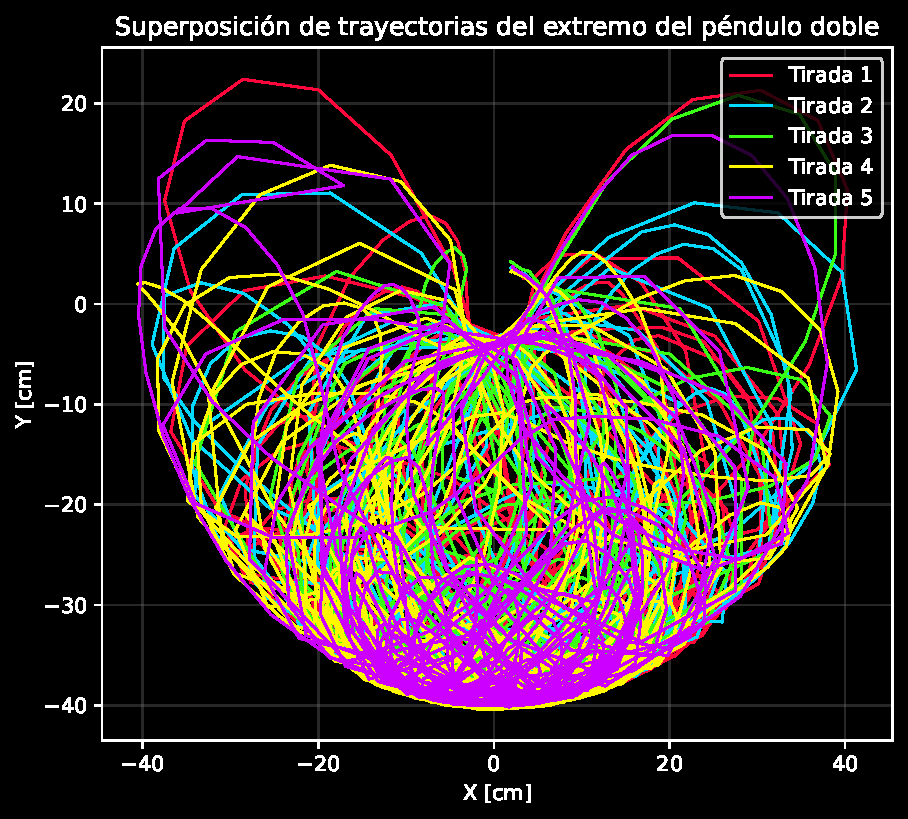
\includegraphics[keepaspectratio]{02-pendulo-doble/experimentos_files/figure-pdf/cell-2-output-1.pdf}}

Esta es la animación que represente la trayectoria que han seguido tres
tiradas. El tiempo que aparece es el tiempo que ha pasado realmente, ya
que la trayectoria está ralentizada para que sea más fácil seguir como
van divergiendo.

\href{?var:site-url/02-pendulo-doble/trayectorias.gif}{Ver animación en
la web}

\section{Comparación con el péndulo
simple}\label{comparaciuxf3n-con-el-puxe9ndulo-simple}

A continuación vamos a mostrar cinco tiradas del péndulo simple. El
péndulo es el mismo que en el caso anterior, lo único que fijamos el
pivote central para que no se mueva, por lo que pasamos de tener un
péndulo doble a uno simple. Igual que en el caso anterior, seguimos el
extremo con el punto rojo.

Como podemos ver en la siguiente figura, a pesar de lanzarse cada una de
las veces desde posiciones ligeramente distintas, las trayectorias son
idénticas.

\pandocbounded{\includegraphics[keepaspectratio]{02-pendulo-doble/experimentos_files/figure-pdf/cell-3-output-1.pdf}}

Y si miramos en la animación el ángulo del péndulo en cada una de las
trayectorias, vemos de nuevo que en función del tiempo las trayectorias
son muy similares.

\href{?var:site-url/02-pendulo-doble/theta_vs_time.gif}{Ver animación en
la web}

He hecho este mismo gráfico con los datos de las tiradas del péndulo
doble. El contraste con el péndulo doble es mayúsculo. En el péndulo
doble no había ni una sola trayectoria idéntica, divergían
continuamente. En el péndulo simple se ve como van iguales.

\href{?var:site-url/02-pendulo-doble/theta_vs_time_doble.gif}{Ver
animación en la web}

\part{La Meteorología y el Caos}

\chapter{Meteorología y Caos}\label{meteorologuxeda-y-caos}

\section{Introducción}\label{introducciuxf3n-5}

A lo largo del proyecto hemos visto la manifestación del caos en modelos
matemáticos como el mapa logístico, o en sistemas físicos como el
péndulo doble.

Uno de los retos del proyecto está en ver la manifestación del caos en
la meteorología. Para ello vamos a proceder de dos maneras:

En la primera de ellas haremos una medida indirecta de la influencia del
caos en las predicciones meteorologicas. Durante varias semanas hemos
recopilado predicciones meteorológicas para Galapagar, y contrastaremos
estás predicciones con las observaciones realizadas para esos días. De
esta manera veremos cómo divergen a medida que pasa el tiempo las
predicciones anteriores. Dado que la atmósfera es un sistema caótico,
cualquier pequeña desviación en las condiciones iniciales estimadas se
amplifica a medida que van pasando los días debido a la actuación del
caos.

En la segunda haremos una estimación directa de un parámetro que hemos
visto que identifica claramente la existencia de caos en un sistema. Se
trata del exponente de Lyapunov. Cogeremos variables meteorológicas
observadas y estimaremos su exponente de Lyapunov, esperando que sea
positivo.

\chapter{Predicitibilidad de datos
meteorológicos}\label{predicitibilidad-de-datos-meteoroluxf3gicos}

El primer paso a la hora de estudiar el caos en el tiempo meteorológico
es disponer de datos históricos de los principales parámetros del
tiempo. Existe una excelente web llamada
\href{https://open-meteo.com/en/docs}{OpenMeteo} que proporciona datos
históricos de observaciones y predicciones para cualquier localidad, y
que además lo hace de forma gratuita en:

https://open-meteo.com/en/docs

Poniéndome manos a la obra, he descargado los datos históricos de
Galapagar desde el año 1950. La serie histórica que devuelve la página
web tiene este formato:

latitude,longitude,elevation,utc\_offset\_seconds,timezone,timezone\_abbreviation\\
40.597538,-4.0735474,885.0,7200,Europe/Berlin,GMT+2

time,temperature\_2m\_mean (°C),precipitation\_sum
(mm),wind\_speed\_10m\_mean (km/h)\\
1950-06-07,20.7,0.50,13.1\\
1950-06-08,18.4,2.30,14.4\\
1950-06-09,18.6,3.10,10.0\\
1950-06-10,18.6,3.90,7.8\\
1950-06-11,18.8,0.50,11.2\\
1950-06-12,17.0,0.00,9.0\\
1950-06-13,18.9,0.20,7.2\\
1950-06-14,21.1,0.00,8.0\\
1950-06-15,20.2,0.00,12.8

En segundo lugar tenemos que saber qué hacer con estos datos. Después de
varias búsquedas en ChatGPT y google encontré un artículo sencillo sobre
cómo calcular el exponente de Lyapunov en datos meteorologicos.

\begin{quote}
\textbf{Referencia completa:} Özgür E. \& Yılmaz M. U. (2022). Using
Chaos Theory to Determine Average Prediction Times of Different
Meteorological Variables: A Case Study in Sivas. \emph{Int. J. Adv. Eng.
Pure Sci.} 34(1):101--106.
\end{quote}

El artículo investiga cuánto tiempo, en promedio, pueden predecirse
fiablemente tres series diarias (temperatura, velocidad del viento y
humedad relativa desde el año 2006 hasta el 2010 para la estación de
Sivas en Turquía) usando teoría del caos. Le pasé este artículo a
chatGPT y le pedí que reprodujese los cálculos para mis datos de
Galapagar. Una de las preguntas que me lanzó de vuelta chatGPT es que si
quería usar los valores de los parámetros \(m\) y \(\tau\) que usaban en
el estudio de la estación turca. Pedí de vuelta a ChatGPT que eran estos
valores, pues al parecer jugaban un papel crítico a la hora de estimar
el valor del exponente de Lyapunov.

\section{\texorpdfstring{Explicación de \(\tau\) y
\(m\)}{Explicación de \textbackslash tau y m}}\label{explicaciuxf3n-de-tau-y-m}

\textbf{Retraso \(\tau\)}\\
El retraso \(\tau\) indica cuántos pasos (días) ``saltamos'' entre cada
coordenada al calcular el exponente de Lyapunov. En lugar de usar solo
\(x(t)\), usamos\\
\[
\bigl(x(t),\,x(t+\tau),\,x(t+2\tau),\dots\bigr).
\]\\
- Si \(\tau\) es muy pequeño, \(x(t)\) y \(x(t+\tau)\) están muy
correlacionados y aportan información casi redundante.\\
- Si \(\tau\) es muy grande, \(x(t)\) y \(x(t+\tau)\) pueden ser casi
independientes y perder la conexión dinámica.

El artículo turco revela que es óptimo trabajar con un valor de \(\tau\)
igual a 3 para la temperatura. Es decir, analizaremos el exponente de
Lyapunov de la serie que nos da la temperatura en Galapagar cada tres
días.

\textbf{Dimensión de embedding \(m\)}\\
La dimensión \(m\) es el número de valores escalonados que usamos para
describir el estado del sistema:\\
\[
\mathbf X(t)=\bigl(x(t),\,x(t+\tau),\,x(t+2\tau),\dots,x(t+(m-1)\tau)\bigr).
\]

Es decir, el estado del sistema en un día, no es solamente el valor de
la temperatura ese día, sino el valor de ese día más varios días
anteriores. Pues bien, lo que necesitamos saber es cual es la dimensión
óptima del estado del sistema. Si por ejemplo solo cojo un día, habrá
muchos días que sean similares ya que habrá muchos casos en los que
coincida la temperatura media para ese día. Sin embargo esto es
engañoso, ya que no se tiene en cuenta el estado pasado del sistema. No
es lo mismo estar en un día a 15 grados de temperatura media después de
haber pasado una ola de calor, que estár a 15 grados después de varios
días de ola de frío. De acuerdo al artículo turco un valor de \(m=12\)
es óptimo.

Con estos valores de \(\tau\) y \(m\) le pedí a ChatGPT que me calculase
el exponente de Lyapunov de la serie de temperaturas de Galapagar.
ChatGPT usa en este caso el mismo algoritmo que para el cálculo del
exponente de Laypunov de las simulaciones del péndulo doble. Se trata de
un algoritmo bastante complicado cuya comprensión se me escapa. Hay que
tener en cuenta que todos estos cálculos los realizo a con el modelo
04-mini-high, que tiene una capacidad matemática muy superior a la
esperada de un alumno de bachillerato, y que además es capaz de hacer
los cálculos en un entorno interno de Python, y de plotear resultados.

\section{Exponente de Lyapunov para la serie de valores de
temperatura}\label{exponente-de-lyapunov-para-la-serie-de-valores-de-temperatura}

A continuación muestro todos los valores de temperatura que hemos sacado
de la web open-meteo. Obviamente en la serie original vemos que hay un
componente estacional muy fuerte. Le pedía ChatGPT que estimase la
variación estacional y que la quitase de los datos, dándome la gráfica
de temperatura desestacionalizada. En ella se ven las variaciones de
temperatura como algo más aleatorio ya que hemos quitado las componentes
estacionales. No obstante se ve una ligera subida de temperaturas desde
el año 1950 hasta el presente, coincidente con el aumento de
temperaturas observado a nivel global en la Tierra.

\pandocbounded{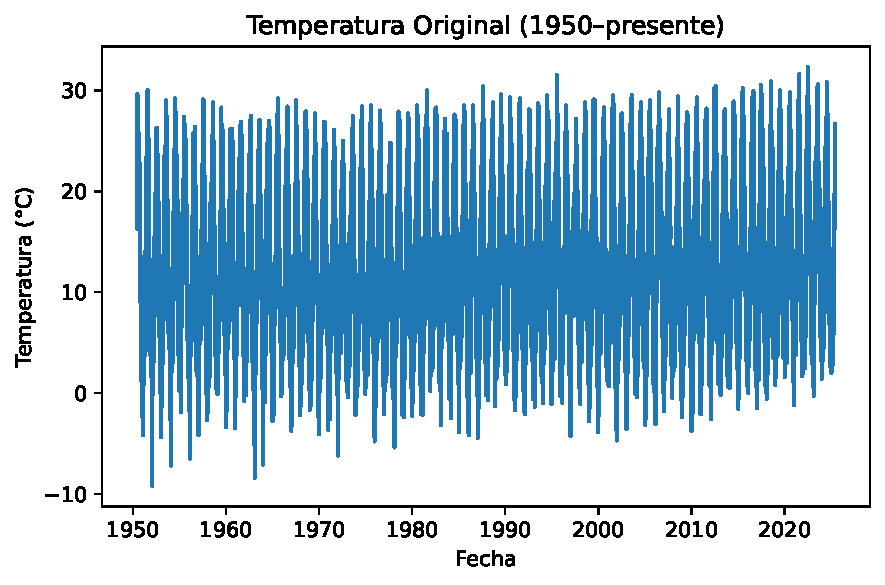
\includegraphics[keepaspectratio]{03-meteorologia/calculolyapunov_files/figure-pdf/cell-2-output-1.pdf}}

\pandocbounded{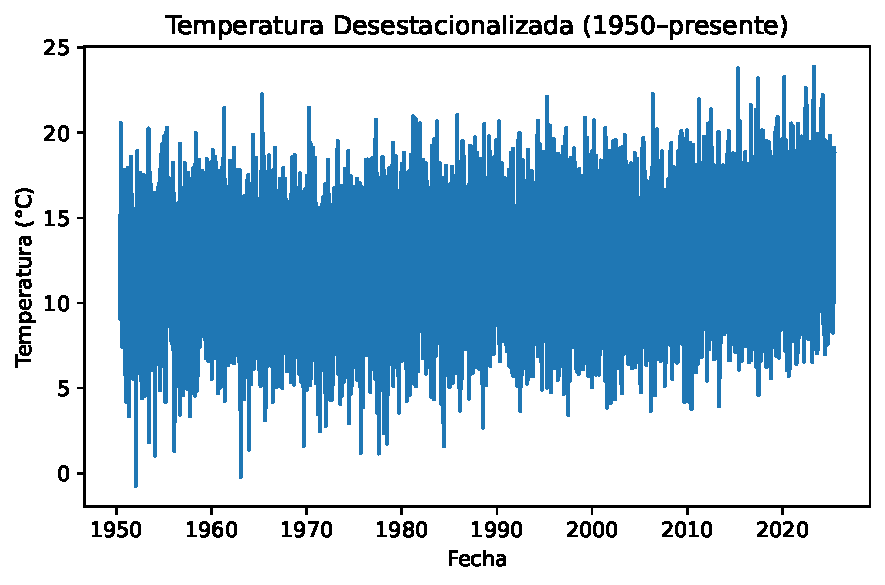
\includegraphics[keepaspectratio]{03-meteorologia/calculolyapunov_files/figure-pdf/cell-2-output-2.pdf}}

Como curiosidad, le pedía a ChatGPT que hiciese una regresión no lineal
de orden 2 para ver como ha ido evolucionando la temperatura media en
Galapagar desde 1950.

\pandocbounded{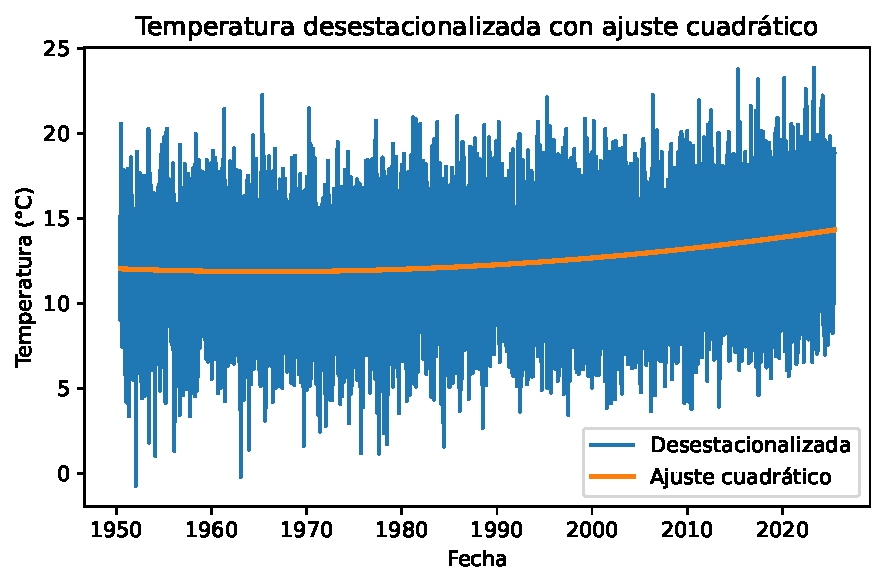
\includegraphics[keepaspectratio]{03-meteorologia/calculolyapunov_files/figure-pdf/cell-3-output-1.pdf}}

La temperatura media desestacionalizada ha subido desde 1950 hasta 2025
aproximadamente
\(\Delta y = y(2025) - y(1950) \approx 2.23\ ^\circ\mathrm{C}\).\\
La tasa media de incremento es
\(\displaystyle \frac{2.23\ ^\circ\mathrm{C}}{75\ \mathrm{años}} \approx 0.030\ ^\circ\mathrm{C}/\mathrm{año}\)
(aproximadamente \(0.3\ ^\circ\mathrm{C}/\mathrm{década}\)). ¡Casi
nada!!!!!

Volvamos al tajo. Ahora le pido a ChatGPT que me haga el cálculo del
exponente de Lyapunov para estos datos de temperatura, usando el mismo
procedimiento y parámetros que en el artículo de la estación de Turquía.
El exponente de Lyapunov máximo calculado para la temperatura
desestacionalizada es\\
\[
\lambda_{\max} \approx 0.219\ \mathrm{día}^{-1}.
\]

\subsection{Horizonte de
predictibilidad}\label{horizonte-de-predictibilidad-1}

Veamos en qué se traduce esta exponente de Lyapunov. Al ser positivo
sabemos que indica que estamos ante un sistema caótico, y que los
errores se amplificarán con el tiempo. Veamos cuando multiplicamos por
10 un error inicial de 0.1 grados Centígrados:

\[
T = \frac{1}{\lambda_{\max}}\ln\Bigl(\frac{L}{\varepsilon}\Bigr)
  = \frac{1}{0.219}\ln(10) \approx 10.5\ \mathrm{días}.
\]

\subsection{Amplificación de un error inicial de 0.1 °C tras 15
días}\label{amplificaciuxf3n-de-un-error-inicial-de-0.1-c-tras-15-duxedas}

Y ahora veamos de formá gráfica cómo se va amplificando el error inicial
de 0.1 grados tras quince días.

\pandocbounded{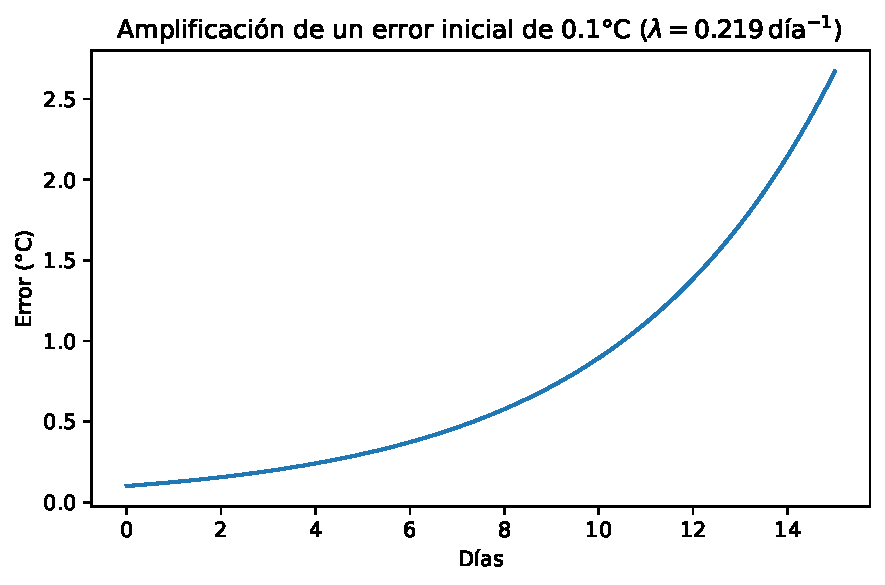
\includegraphics[keepaspectratio]{03-meteorologia/calculolyapunov_files/figure-pdf/cell-4-output-1.pdf}}

Estos valores refuerzan las hipótesis inciales con las que habíamos
especulado. Pasadas dos semanas es muy difícil tener estimaciones
precisas del tiempo meteorológico.

\section{Exponente de Lyapunov para la serie de velocidad del
viento}\label{exponente-de-lyapunov-para-la-serie-de-velocidad-del-viento}

A continuación cargamos y desestacionalizamos los datos de velocidad del
viento (1950--presente), mostramos la serie original y la
desestacionalizada:

\pandocbounded{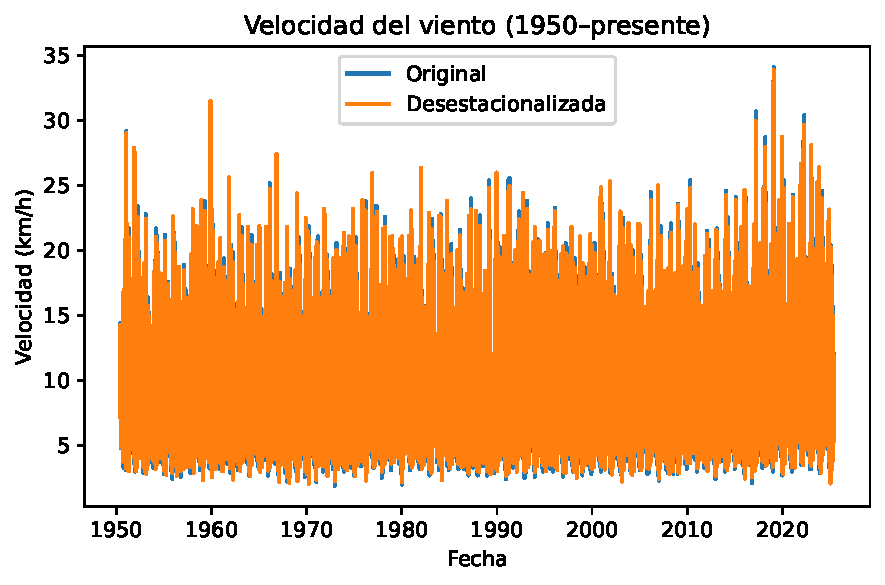
\includegraphics[keepaspectratio]{03-meteorologia/calculolyapunov_files/figure-pdf/cell-5-output-1.pdf}}

En este caso no hay gran diferencia entre la componente
desestacionalizada y sin desestacionalizar.

\subsection{Exponente de Lyapunov}\label{exponente-de-lyapunov}

El exponente de Lyapunov máximo calculado para la serie de viento
desestacionalizada (usando Wolf, \(m=12\), \(\tau=3\)) es\\
\[
\lambda_{\max} \approx 0.414\ \mathrm{día}^{-1}.
\]

\subsection{Horizonte de
predictibilidad}\label{horizonte-de-predictibilidad-2}

Para un error inicial \(\varepsilon = 1\ \mathrm{km/h}\) y un factor de
crecimiento 10× (\(L/\varepsilon=10\)):\\
\[
T = \frac{1}{\lambda_{\max}}\ln\Bigl(\frac{L}{\varepsilon}\Bigr)
  = \frac{1}{0.414}\ln(10)\approx5.6\ \mathrm{días}.
\]

\subsection{Amplificación de un error inicial de 1 km/h tras 15
días}\label{amplificaciuxf3n-de-un-error-inicial-de-1-kmh-tras-15-duxedas}

\pandocbounded{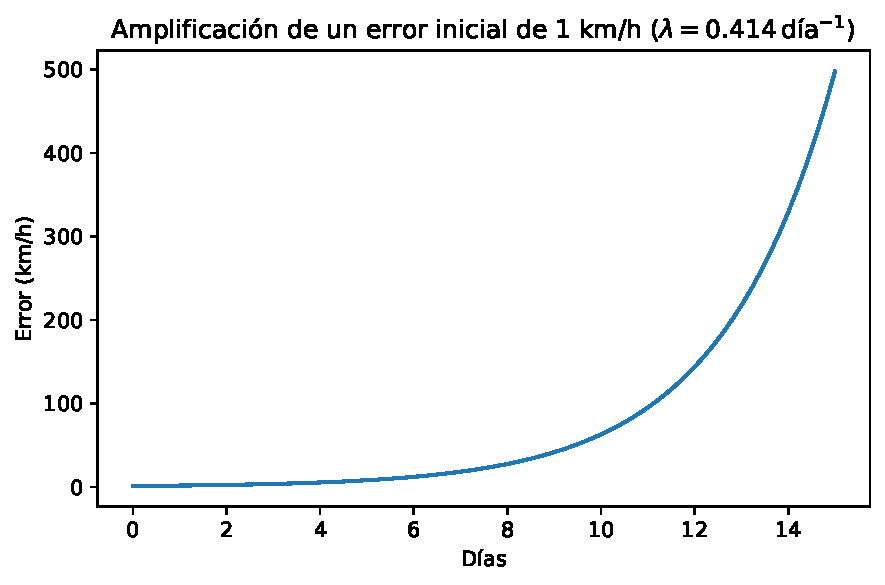
\includegraphics[keepaspectratio]{03-meteorologia/calculolyapunov_files/figure-pdf/cell-6-output-1.pdf}}

\subsection{Comparación de la predictibilidad: viento vs
temperatura}\label{sec-lyapunov}

En el caso de la temperatura desestacionalizada, obtuvimos un exponente
de Lyapunov\\
\[
\lambda_{\max}^{\rm temp}\approx0.219\ \mathrm{día}^{-1},
\]\\
lo que da un horizonte de predictibilidad de\\
\[
T_{\rm temp}
=\frac{1}{0.219}\ln(10)\approx10.5\ \mathrm{días}.
\]

Para la velocidad del viento desestacionalizada hallamos\\
\[
\lambda_{\max}^{\rm viento}\approx0.414\ \mathrm{día}^{-1},
\]\\
y por tanto\\
\[
T_{\rm viento}
=\frac{1}{0.414}\ln(10)\approx5.6\ \mathrm{días}.
\]

Observamos que\\
\[
T_{\rm viento}\approx\frac{1}{2}\,T_{\rm temp}.
\]\\
Esto significa que \textbf{la serie de viento es más caótica}: su
exponente de Lyapunov es casi el doble, y los errores iniciales se
amplifican mucho más rápido.

Varias razones explican esta diferencia:

\begin{itemize}
\tightlist
\item
  \textbf{Variabilidad a corto plazo}: la velocidad del viento está
  dominada por fenómenos de escala reducida (frentes, turbulencia,
  ráfagas) que inducen cambios bruscos.
\item
  \textbf{Forzamientos estacionales débiles}: el ciclo anual aporta poca
  oscilación comparado con la temperatura, por lo que el viento muestra
  un comportamiento intrínsecamente más errático.
\end{itemize}

\begin{enumerate}
\def\labelenumi{\arabic{enumi}.}
\item
  \textbf{¿Qué es un ``forzamiento estacional''?}\\
  Es la variación periódica y predecible que se repite cada año, debida
  al cambio de estación (más sol y calor en verano, menos en invierno).
\item
  \textbf{Temperatura vs.~viento}

  \begin{itemize}
  \tightlist
  \item
    \textbf{Temperatura}: el rango típico entre verano e invierno puede
    ser de \(\pm10\ ^\circ\mathrm{C}\) o más. Es decir, el ciclo anual
    supone una parte muy importante de la variabilidad total.\\
  \item
    \textbf{Viento}: la velocidad media cambia solo unos
    \(\pm2\ \mathrm{km/h}\) a lo largo del año. Esa ``señal'' anual es
    pequeña comparada con las oscilaciones diarias o las rachas
    impredecibles.
  \end{itemize}
\item
  \textbf{Efecto al desestacionalizar}

  \begin{itemize}
  \tightlist
  \item
    Al quitar la estacionalidad de la temperatura, reducimos mucho la
    amplitud de la serie y ``dejamos ver'' las fluctuaciones reales.\\
  \item
    Al hacer lo mismo con el viento, casi no cambiamos nada: la mayor
    parte de la variabilidad ya venía de eventos de corto plazo, no del
    ciclo anual.
  \end{itemize}
\end{enumerate}

\begin{itemize}
\tightlist
\item
  \textbf{Implicaciones prácticas}: mientras que las predicciones de
  temperatura pueden ser útiles hasta unos 10 días, las de viento
  pierden precisión ya a los 5--6 días, reflejo de su carácter más
  caótico.
\end{itemize}

\chapter{Caos en las predicciones
meteorológicas}\label{caos-en-las-predicciones-meteoroluxf3gicas}

La meteorología es un ejemplo paradigmático de sistema caótico. Edward
Lorenz, en su famoso artículo de 1963, demostró que pequeñas
perturbaciones en las condiciones iniciales pueden producir divergencias
exponenciales en la evolución del sistema atmosférico (Lorenz, 1963).
Esta propiedad se cuantifica mediante el \textbf{exponente de Lyapunov},
el cual mide la tasa a la que dos trayectorias inicialmente cercanas se
separan en el espacio de fases.

Como ya hemos mencionado uno de los retos del proyecto es demostrar que
el tiempo es un sistema caótico. En la anterior entrada del proyecto
hice un cálculo del exponente de Lyapunov cogiendo medidas reales de
variables como la temperatura y el viento, y analizándolas por medio de
rutinas hechas por ChatGPT. Los valores resultantes eran lo esperado: un
horizonte de predictibilidad de 10 días para la temperatura media
diaria.

Ahora vamos a emprender un método indirecto de cálculo. Las diferentes
organizaciones meteorológicas realizan todos los días predicciones de
hasta 14 días. Puesto que el tiempo es caótico, este caos se tiene que
reflejar en el error de las predicciones. A medida que aumenta la
distancia con respecto al día actual, el error tiene que aumentar. Este
incremento no será lineal sino que será exponencial, de acuerdo a la
teoría que ya hemos visto. Si cogemos los errores, y hacemos un
logaritmo, podremos hacer una regresión lineal del logaritmo del error,
lo que nos dará el exponente de Lyapunov. Así de sencillo. Se trata de
una medida indirecta, pero creo que muy sencilla del exponente de
Lyapunov.

\section{Proceso de Recopilación de Datos Mediante el Script de
Python}\label{proceso-de-recopilaciuxf3n-de-datos-mediante-el-script-de-python}

En este punto lo primero que tenemos que hacer es recopilar datos. En
este caso en vez de usar open-meteo, usé Visual Crossing
(https://www.visualcrossing.com/) , que dispone también de una utilidad
gratuita para descargar previsiones meteorológicas. Para ello, pedí a
ChatGPT que hiciera un script para coger los datos de Visual Crossing.
El script desarrollado tiene dos funciones principales, diseñadas para
ir acumulando la información necesaria a lo largo del tiempo:

\emph{a) Registro de Pronósticos (``Forecast'')}

Cada día se obtiene un pronóstico para 15 días (el día actual + 14 días
de anticipación) a través de la API de Visual Crossing. Para cada
parámetro (temperatura, humedad, presión y velocidad del viento), se
crea un archivo CSV en el que cada fila contiene:

\begin{itemize}
\tightlist
\item
  \textbf{Columna 1:} La fecha de creación del pronóstico (formato
  americano: M-D-YYYY).
\item
  \textbf{Columnas 2 a 15:} Los valores predichos para 1 día adelante, 2
  días adelante, \ldots, hasta 14 días adelante.
\end{itemize}

Matemáticamente, si denotamos por \(F_{\text{param}}(d, n)\) el valor
predicho para el parámetro en el día \(d+n\) cuando el pronóstico se
realizó en el día \(d\), la fila correspondiente al pronóstico realizado
en la fecha \(d\) es:

\[
\text{Fila}_d = \bigl[ d,\; F_{\text{param}}(d,1),\; F_{\text{param}}(d,2),\; \dots,\; F_{\text{param}}(d,14) \bigr]
\]

\emph{b) Registro Retroactivo (``Retro'')}

El propósito de este archivo es reconstruir, para cada día objetivo, la
evolución de los pronósticos hechos en días anteriores y compararlos con
el valor observado real. Para cada parámetro se crea un archivo CSV en
el que cada fila contiene:

\begin{itemize}
\tightlist
\item
  \textbf{Columna 1:} La fecha del día objetivo (por ejemplo, ayer,
  formato M-D-YYYY).
\item
  \textbf{Columna 2:} El valor observado históricamente para ese día.
\item
  \textbf{Columnas 3 a 16:} Los pronósticos para ese mismo día,
  realizados desde 1 hasta 14 días antes.
\end{itemize}

En otras palabras, para un día objetivo \(d_{\text{target}}\), se
recupera el pronóstico realizado en \(d_{\text{target}} - n\) (para
\(n = 1,2,\dots,14\)) y se toma el valor predicho correspondiente al
\(n\)-ésimo día. La fila retroactiva es:

\[
\text{Retro}_d = \bigl[ d_{\text{target}},\; O(d_{\text{target}}),\; F_{\text{param}}(d_{\text{target}}-1,1),\; F_{\text{param}}(d_{\text{target}}-2,2),\; \dots,\; F_{\text{param}}(d_{\text{target}}-14,14) \bigr]
\]

donde \(O(d_{\text{target}})\) es el valor observado real para el
parámetro en el día objetivo.

La estructura de los dos ficheros se detalla en la siguiente figura

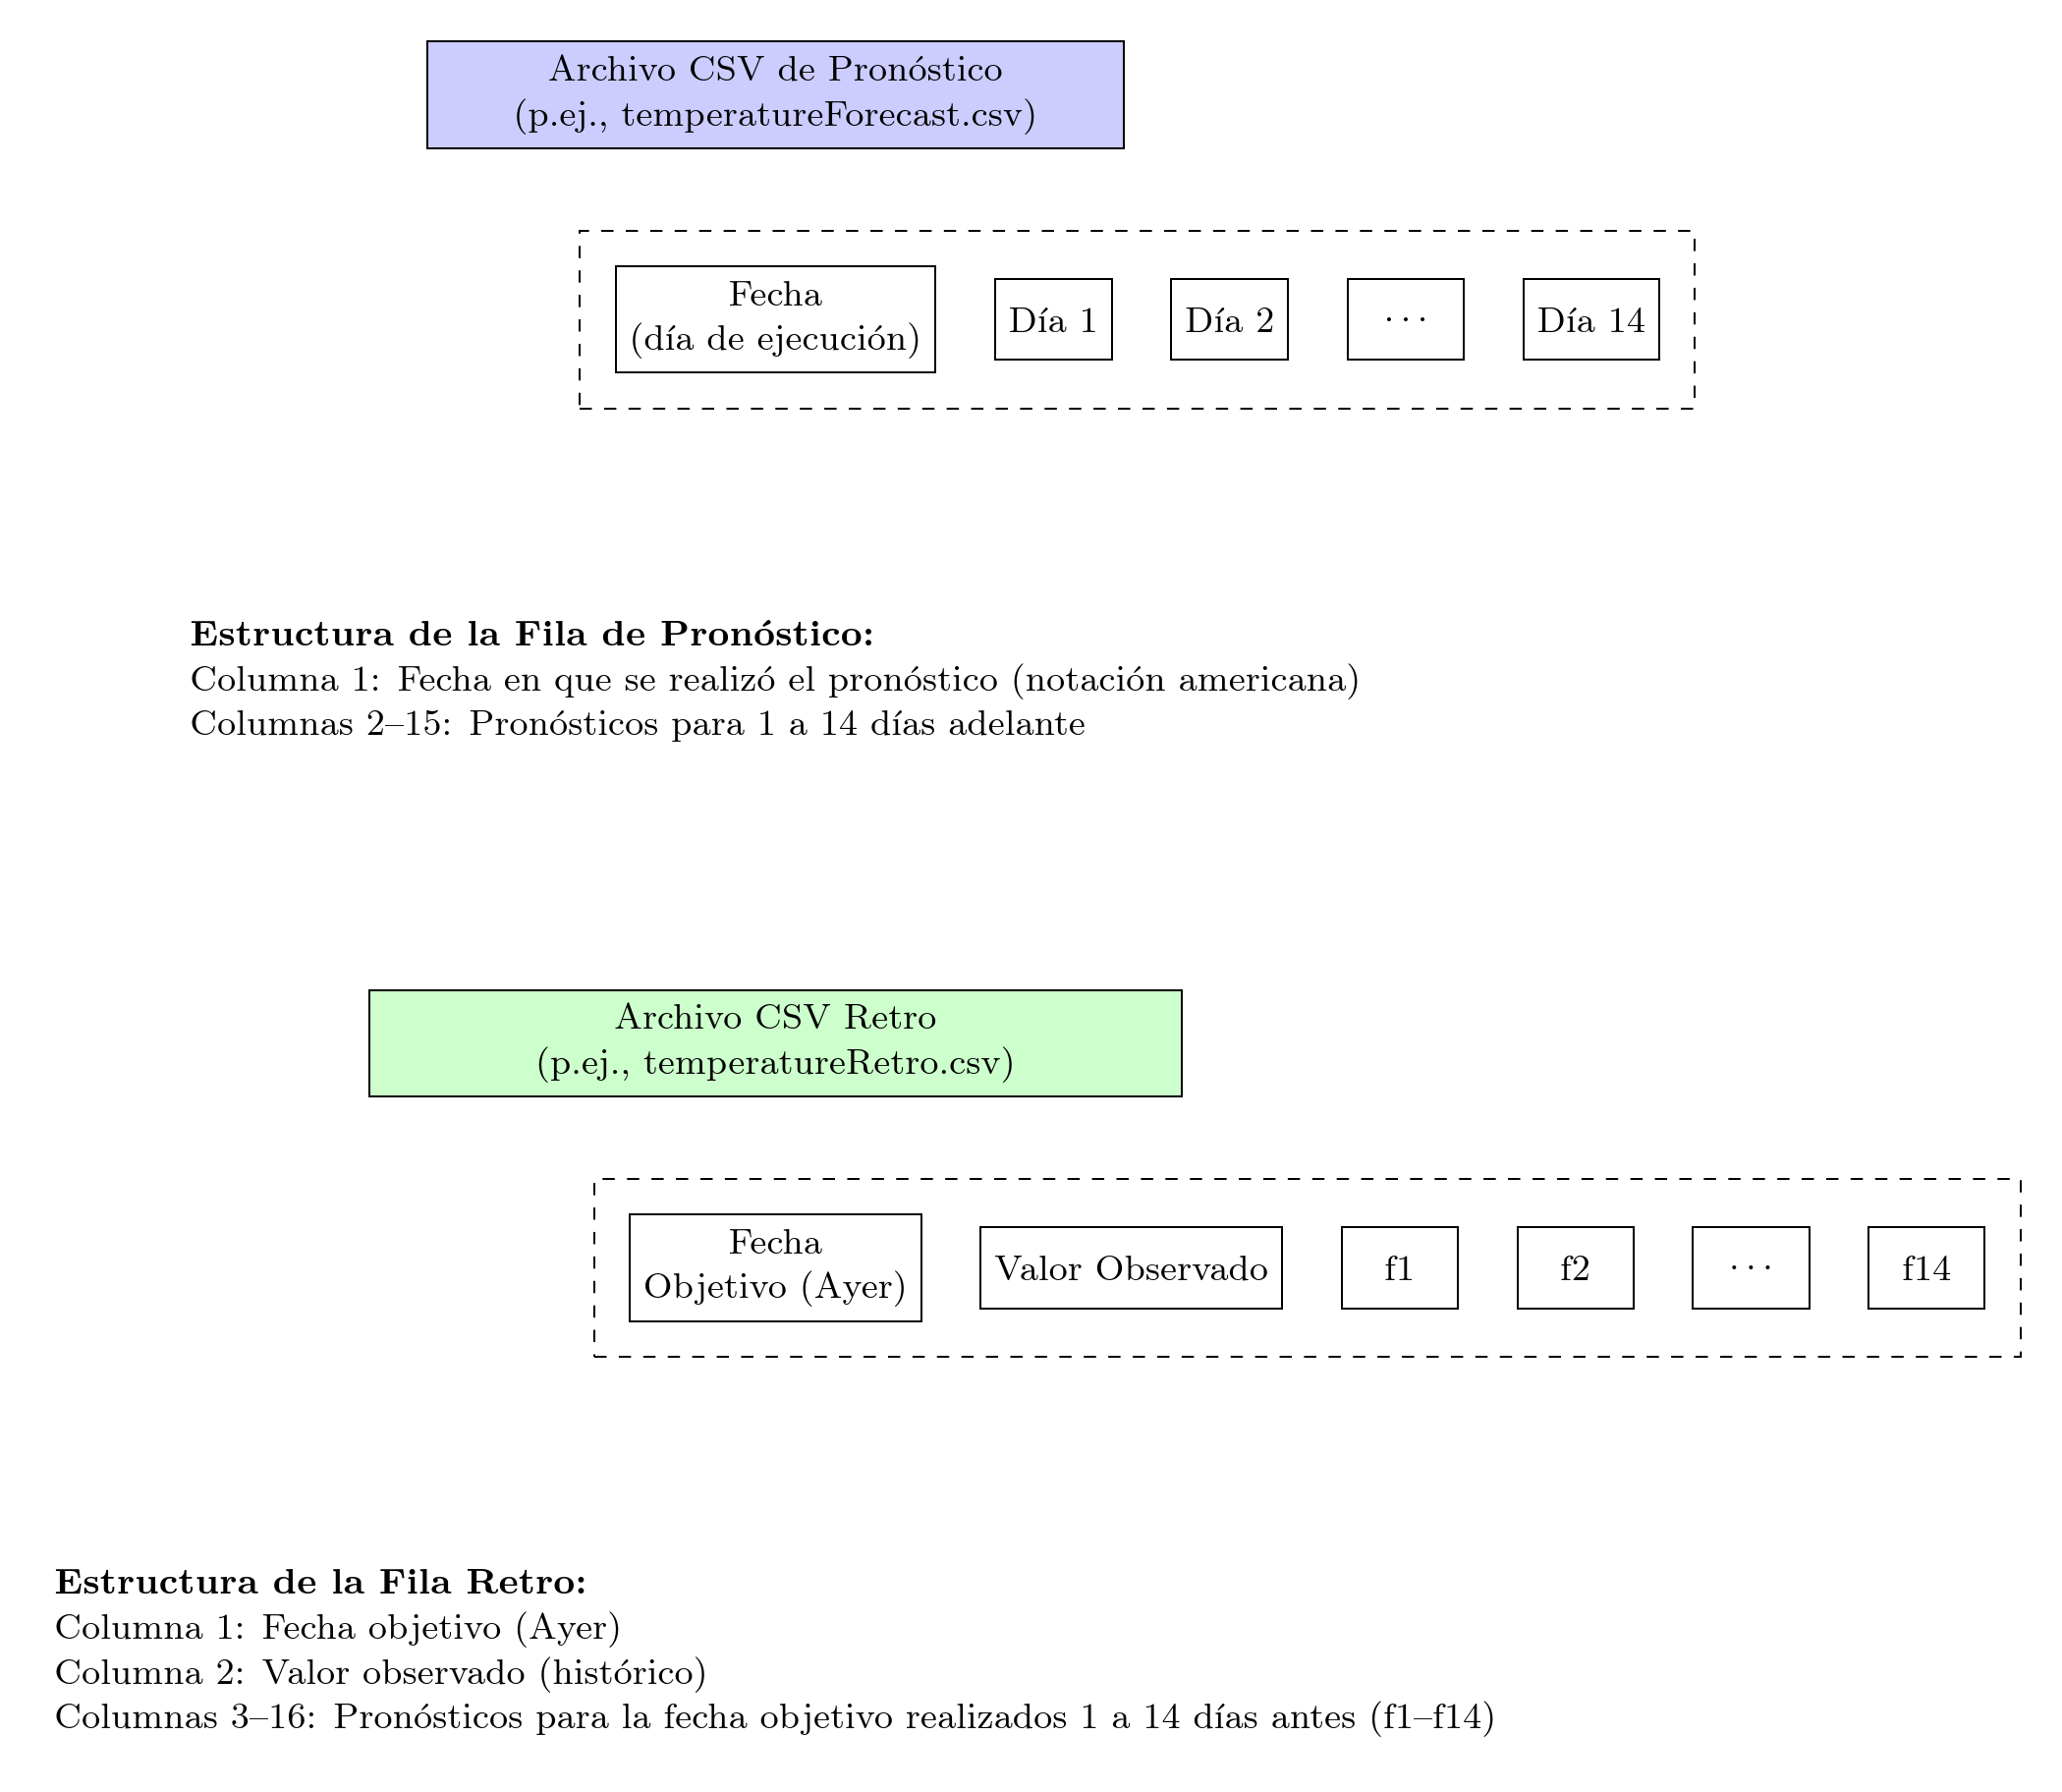
\includegraphics[width=1\linewidth,height=\textheight,keepaspectratio]{03-meteorologia/FicheroCSV.png}

Y el procedimiento que hace el script diariamente se detalla a
continuación.

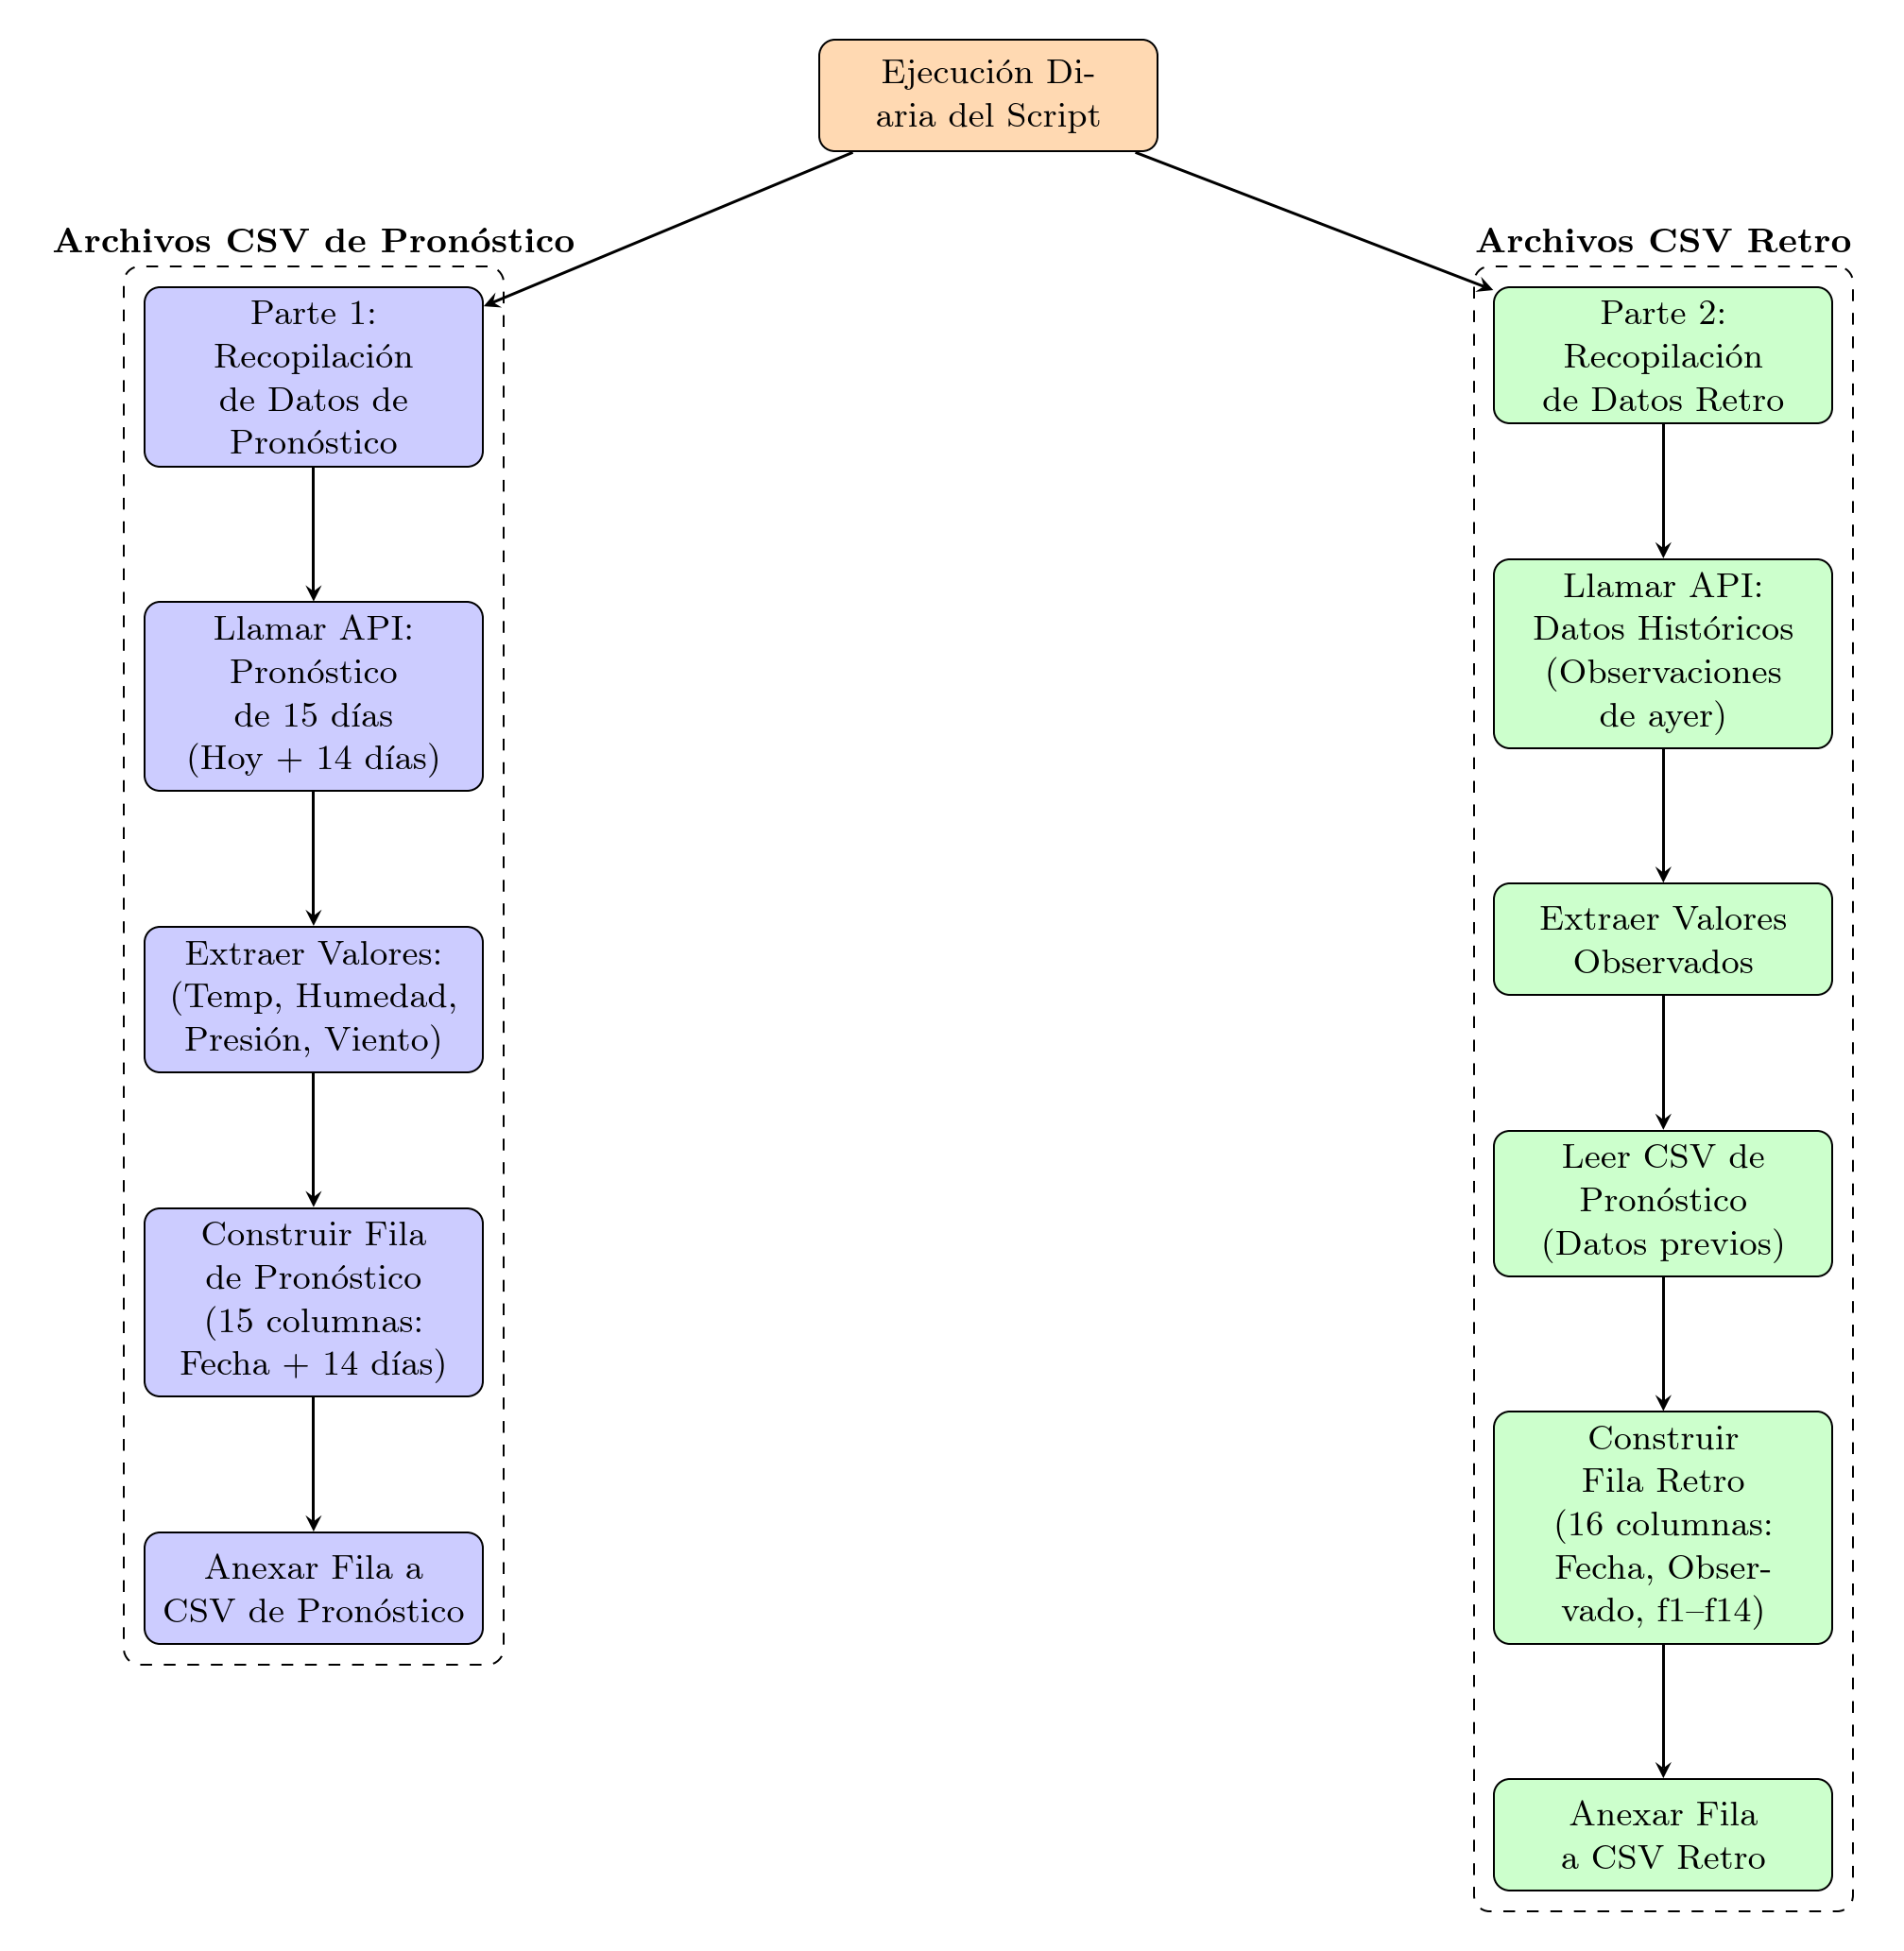
\includegraphics[width=1\linewidth,height=\textheight,keepaspectratio]{03-meteorologia/EjecucionDiaria.png}

El error de cada pronóstico se define como:

\[
e(n) = \bigl| F_{\text{param}}(d_{\text{target}}-n, n) - O(d_{\text{target}}) \bigr|
\]

para \(n = 1,2,\dots,14\). Esta serie \(\{e(n)\}\) representa cómo varía
el error en función del tiempo de anticipación.

\section{Análisis de Datos y Determinación del Coeficiente de
Lyapunov}\label{anuxe1lisis-de-datos-y-determinaciuxf3n-del-coeficiente-de-lyapunov}

\emph{a) Enfoque Teórico Clásico}

En un sistema caótico, la separación entre dos trayectorias evoluciona
de forma exponencial. Asumiendo que el error en el pronóstico \(e(n)\)
crece de manera similar, se modela como:

\[
e(n) = e(0)\, e^{\lambda n}
\]

Tomando logaritmos:

\[
\ln e(n) = \ln e(0) + \lambda n
\]

Por lo tanto, si se realiza un ajuste lineal de \(\ln e(n)\) en función
de \(n\), la pendiente de la recta brinda una estimación empírica de
\(\lambda\).

\emph{b) Enfoque Empírico Propuesto}

En este estudio, en lugar de disponer de dos trayectorias
infinitesimalmente separadas, se utilizan las diferencias en las
predicciones realizadas en distintos días para el mismo objetivo. Cada
error \(e(n)\) se obtiene como la diferencia entre el pronóstico hecho
\(n\) días antes y el valor observado:

\[
e(n) = \bigl| F_{\text{param}}(d_{\text{target}}-n, n) - O(d_{\text{target}}) \bigr|
\]

La estimación empírica del exponente de Lyapunov se obtiene realizando
un ajuste lineal de:

\[
\ln e(n) = \ln e(0) + \lambda_{\text{emp}} n
\]

donde \(\lambda_{\text{emp}}\) es la pendiente obtenida a partir de la
regresión lineal sobre los datos \((n, \ln e(n))\).

Esto ya lo vimos en la sección \hyperref[sec-sensibilidad]{Efecto
mariposa}. En esa sección vimos como el error iba creciendo
exponencialemnte, y al hacer el logaritmo nos quedó una recta cuya
pendiente era el exponente de Lyapunov de la función logística para ese
valor de \(r\). En este caso, veremos que el error de pronóstico crece
también exponencialmente, no linealmente, lo que al hacer el logaritmo
nos permitirá sacar la pendiente y por tanto el exponente de Lyapunov.

\emph{c) Confrontación con la Fórmula Tradicional}

\textbf{Fórmula Tradicional:}

\[
\lambda = \lim_{t \to \infty} \frac{1}{t} \ln \frac{|\delta x(t)|}{|\delta x(0)|}
\]

\textbf{Fórmula Empírica del Estudio:}

\[
\lambda_{\text{emp}} \approx \text{slope}\bigl(\ln e(n)\ \text{vs.}\ n\bigr)
\]

En este caso, \(e(n)\) incorpora tanto la sensibilidad a las condiciones
iniciales como los errores inherentes del modelo de pronóstico. Además,
el análisis se realiza sobre un rango discreto de días (1 a 14), por lo
que \(\lambda_{\text{emp}}\) debe interpretarse como una aproximación de
la tasa de divergencia del error.

\section{Resultados}\label{resultados-2}

Durante los meses de febrero, marzo y abril estuve recopilando las
predicciones y los valores observados de temperatura, humedad, viento y
presión atmosférica para Galapagar.

El conjunto de errores para cada día de la predicción se muestran a
continuación (cada línea representa un día en el que se realiza la
predicción).

\pandocbounded{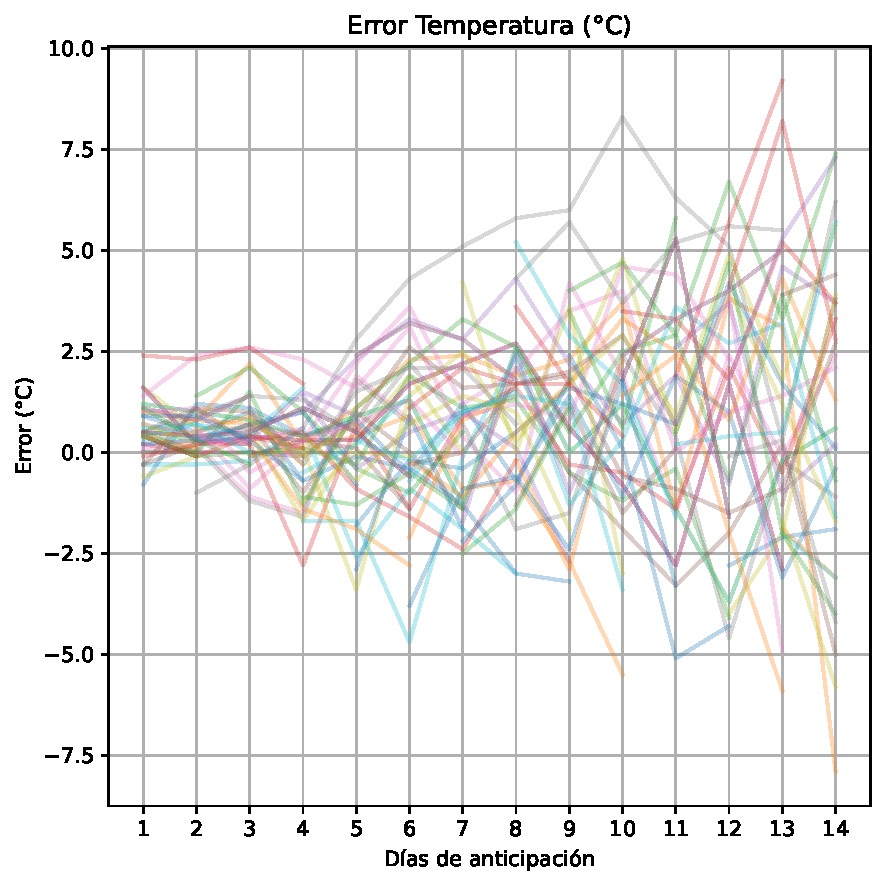
\includegraphics[keepaspectratio]{03-meteorologia/predicciones_files/figure-pdf/cell-2-output-1.pdf}}

\pandocbounded{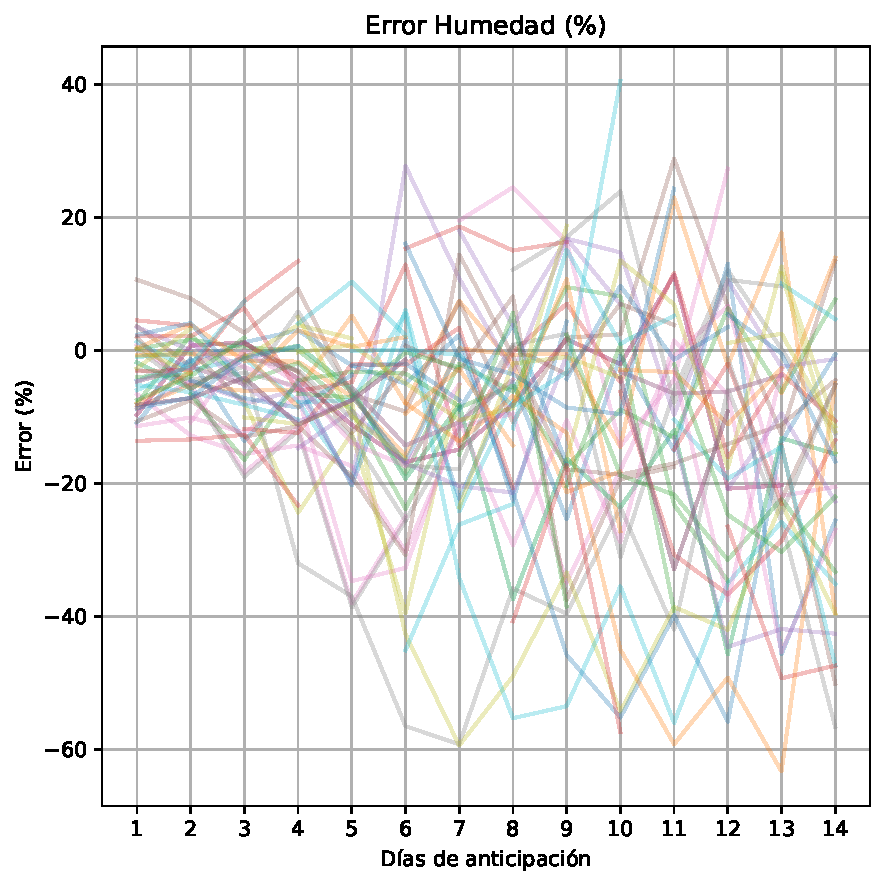
\includegraphics[keepaspectratio]{03-meteorologia/predicciones_files/figure-pdf/cell-2-output-2.pdf}}

\pandocbounded{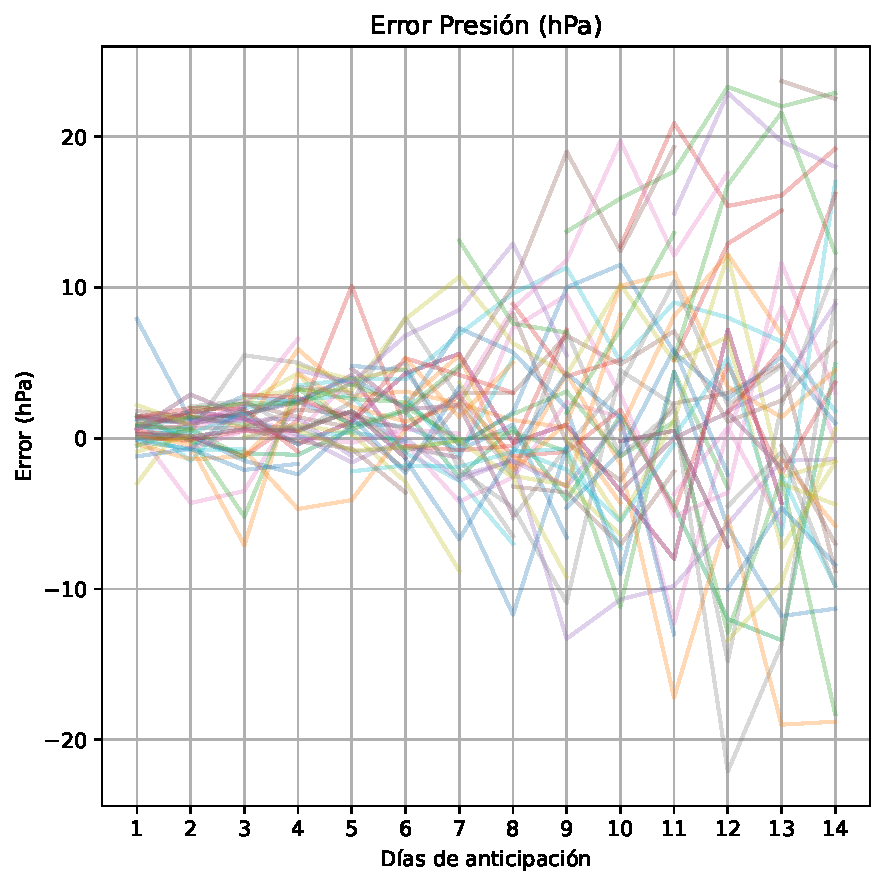
\includegraphics[keepaspectratio]{03-meteorologia/predicciones_files/figure-pdf/cell-2-output-3.pdf}}

\pandocbounded{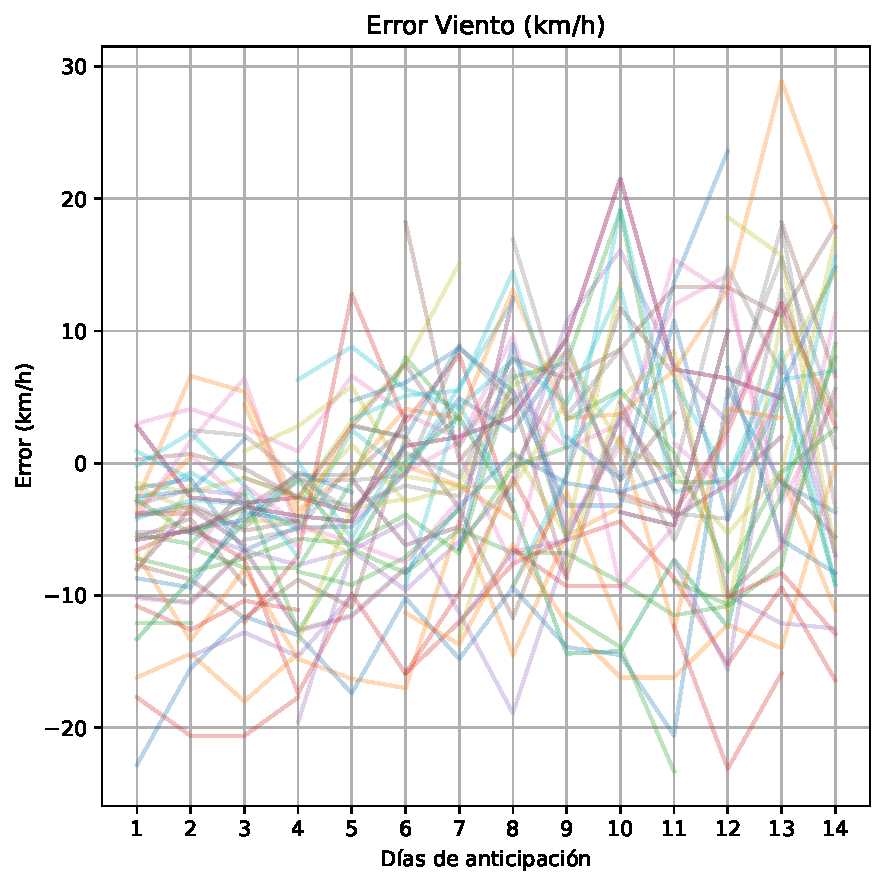
\includegraphics[keepaspectratio]{03-meteorologia/predicciones_files/figure-pdf/cell-2-output-4.pdf}}

Los errores medios en valor absoluto de predicción en función del número
de días anteriores en los que se hizo la predicción se muestran a
continuación. Se ve claramente que los errores van aumentando
exponencialmente.

\pandocbounded{\includegraphics[keepaspectratio]{03-meteorologia/predicciones_files/figure-pdf/cell-3-output-1.pdf}}

\pandocbounded{\includegraphics[keepaspectratio]{03-meteorologia/predicciones_files/figure-pdf/cell-3-output-2.pdf}}

\pandocbounded{\includegraphics[keepaspectratio]{03-meteorologia/predicciones_files/figure-pdf/cell-3-output-3.pdf}}

\pandocbounded{\includegraphics[keepaspectratio]{03-meteorologia/predicciones_files/figure-pdf/cell-3-output-4.pdf}}

Y ahora le pedimos a ChatGPT que nos calcule el exponente de Lyapunov, y
que nos trace de forma superpuesta el error de acuerdo al exponente de
Lyapunov.

\pandocbounded{\includegraphics[keepaspectratio]{03-meteorologia/predicciones_files/figure-pdf/cell-4-output-1.pdf}}

\pandocbounded{\includegraphics[keepaspectratio]{03-meteorologia/predicciones_files/figure-pdf/cell-4-output-2.pdf}}

\pandocbounded{\includegraphics[keepaspectratio]{03-meteorologia/predicciones_files/figure-pdf/cell-4-output-3.pdf}}

\pandocbounded{\includegraphics[keepaspectratio]{03-meteorologia/predicciones_files/figure-pdf/cell-4-output-4.pdf}}

Los exponentes de Lyapunov salen más pequeños que los calculados
mediante las series históricas en la sección anterior
\hyperref[sec-lyapunov]{Predictibilidad}. Hay que tener en cuenta que
los exponentes en la sección anterior se tomaban sobre la base de 75
años, mientras que aquí tenemos un experimento más limitado, solamente
tres meses, por lo que es normal que no cuadren del todo los datos. Sin
embargo, tal y como hipotizamos, estamos alredededor de las dos semanas
como límite de predictbilidad.

Además lo que es muy relevante, es ver como el error de predicción crece
exponencialmente. Se ponen de manifiesto dos causas: la inexactitud de
las condiciones inciales, y la inexactitud de los modelos y sus
cómputos. Puesto que el sistema modelado es caótico, tal y como
esperabamos los errores crecen exponencialmente.

\section{Referencias
Bibliográficas}\label{referencias-bibliogruxe1ficas}

\chapter{Entrevista con expertos de la
AEMET}\label{entrevista-con-expertos-de-la-aemet}

El Jueves 19 de Junio tuve la oportunidad de tener una entrevista con
dos meteorólogos de la Agencia Estatal de Meteorología para hacerles
algunas preguntas sobre la parte del proyecto donde se estudia el caos
en la predicción meteorológica y climática. De esta manera he podido
incluir también la opinión de expertos en el tema en este proyecto. Aquí
están todas las preguntas que hice durante la entrevista y cuáles fueron
las respuestas de los expertos:

\section{¿Qué condiciones atmosféricas hacen que el sistema sea más
caótico y por tanto que sea más difícil llevar a cabo una predicción
meteorológica fiable, y cuales lo hacen más
fácil?}\label{quuxe9-condiciones-atmosfuxe9ricas-hacen-que-el-sistema-sea-muxe1s-cauxf3tico-y-por-tanto-que-sea-muxe1s-difuxedcil-llevar-a-cabo-una-predicciuxf3n-meteoroluxf3gica-fiable-y-cuales-lo-hacen-muxe1s-fuxe1cil}

Las condiciones en las que la atmósfera es más inestable como borrascas
o ambientes de tormenta, porque es más difícil establecer unas
condiciones iniciales que no tengan mucho error y que sean precisas.
Esto hace que el error inicial en las mediciones sea grande y que se
propague más rápidamente.

\section{¿Existe un horizonte de predictibilidad a partir del cual las
predicciones meteorológicas no van a llegar a ser fiables nunca sin
importar los avances tecnológicos y en los modelos que se puedan llevar
a cabo en el futuro? ¿Cuál consideráis que es el horizonte de
predictibilidad
actualmente?}\label{existe-un-horizonte-de-predictibilidad-a-partir-del-cual-las-predicciones-meteoroluxf3gicas-no-van-a-llegar-a-ser-fiables-nunca-sin-importar-los-avances-tecnoluxf3gicos-y-en-los-modelos-que-se-puedan-llevar-a-cabo-en-el-futuro-cuuxe1l-consideruxe1is-que-es-el-horizonte-de-predictibilidad-actualmente}

Sí, existe un horizonte de predictibilidad en meteorología, y es teórico
y práctico al mismo tiempo. Se trata de un límite físico-matemático
impuesto por la naturaleza del sistema atmosférico: un sistema caótico y
no lineal. Este límite está alrededor de los 20 días y no importa cuán
potentes sean los ordenadores del futuro o lo precisos que sean los
sensores, este límite no va a poder superarse.

\section{¿Qué avances tecnológicos o metodológicos han mejorado más la
capacidad predictiva frente a la naturaleza caótica de la
atmósfera?}\label{quuxe9-avances-tecnoluxf3gicos-o-metodoluxf3gicos-han-mejorado-muxe1s-la-capacidad-predictiva-frente-a-la-naturaleza-cauxf3tica-de-la-atmuxf3sfera}

Los satélites, ya que permiten toar mediciones de las diferentes capas
de la atmósfera con más facilidad y de zonas más amplias que los globos
meteorológicos, la capacidad computacional de los superordenadores y que
se van añadiendo nuevos términos a las ecuaciones que dan más detalle y
ayudan a mejorarlas.

\section{¿Existe algún parámetro como precipitación, viento, temperatura
o humedad que sea más difícil de predecir y más caótico que otro o por
el contrario más fácil de predecir que
otro?}\label{existe-alguxfan-paruxe1metro-como-precipitaciuxf3n-viento-temperatura-o-humedad-que-sea-muxe1s-difuxedcil-de-predecir-y-muxe1s-cauxf3tico-que-otro-o-por-el-contrario-muxe1s-fuxe1cil-de-predecir-que-otro}

Si, los parámetros que son derivados de los demás que se obtienen
sabiendo otros como la precipitación o la nubosidad, ya que no salen
directamente de las ecuaciones que se utilizan en las predicciones, si
no que se obtienen teniendo en cuenta mucho parámetros más simples que
si salen de las ecuaciones

\section{¿Cómo se tiene en cuenta el error que existe a la hora de hacer
las simulaciones de la atmósfera, que vienen dados por el propio límite
de los ordenadores en cuanto a precisión en los
decimales?}\label{cuxf3mo-se-tiene-en-cuenta-el-error-que-existe-a-la-hora-de-hacer-las-simulaciones-de-la-atmuxf3sfera-que-vienen-dados-por-el-propio-luxedmite-de-los-ordenadores-en-cuanto-a-precisiuxf3n-en-los-decimales}

No existe ningún método como tal para reducir o eliminar ese error pero
muchas veces no se llega a aprovechar toda la precisión que te permite
el ordenador ya que los cálculos llevan mucho tiempo, y muchas veces se
necesitan tener terminadas las predicciones rápidamente.

\section{¿Existe sensibilidad a las condiciones iniciales en las
predicciones climáticas a largo plazo de la misma manera que en la
predicción meteorológica, donde acaban dando lugar al
caos?}\label{existe-sensibilidad-a-las-condiciones-iniciales-en-las-predicciones-climuxe1ticas-a-largo-plazo-de-la-misma-manera-que-en-la-predicciuxf3n-meteoroluxf3gica-donde-acaban-dando-lugar-al-caos}

Si existe pero las condiciones iniciales afectan menos ya que las
ecuaciones utilizadas se simplifican y se vuelven lineales. Por otra
parte el resultado no tiene que ser tan preciso ya que lo que se obtiene
es una media. Sin embargo, aunque no sea casi caótico sigue siendo
difícil establecer las condiciones iniciales por lo que el error inicial
puede acabar propagándose aunque más lentamente que en las predicciones
meteorológicas.

\section{¿Existe alguna condición o tipo de clima el cual presenta más o
menos caos a la hora de realizar predicciones a largo
plazo?}\label{existe-alguna-condiciuxf3n-o-tipo-de-clima-el-cual-presenta-muxe1s-o-menos-caos-a-la-hora-de-realizar-predicciones-a-largo-plazo}

Sí que existen algunos climas que son más predecibles que otros a largo
plazo. En predicción climática, el caos no desaparece, pero su impacto
depende mucho del contexto:Si una región está controlada por
forzamientos globales regulares, como El Niño, es menos caótica y más
predecible. Si depende del ruido interno de la atmósfera o de factores
locales, el caos reina y la predictibilidad climática estacional es
baja.

\section{¿Es el caos la razón de que algunas de las predicciones
climatológicas hechas hace varias décadas no hayan sido muy precisas o
incluso algunas hayan llegado a
fallar?}\label{es-el-caos-la-razuxf3n-de-que-algunas-de-las-predicciones-climatoluxf3gicas-hechas-hace-varias-duxe9cadas-no-hayan-sido-muy-precisas-o-incluso-algunas-hayan-llegado-a-fallar}

Sí puede serlo algunas veces, aunque también influyen muchos factores
externos como la actividad humana que no se pueden predecir.

\part{El Clima y el Caos}

\chapter{Clima}\label{clima}

Llegamos a la parte más cualitativa y menos cuantitativa del proyecto,
no por ello menos importante. Como bien se manifiesta en los medios de
comunicación y en la comunidad científica la predicción del clima es uno
los puntos más importantes para la humanidad. Si bien en el capítulo
anterior hemos investigado sobre como afecta el caos a la previsión
meteorológica ahora vamos a hacer lo mismo con el clima.

Con el tiempo meteorológico a corto plazo todo el mundo asume que las
previsiones meteorológicas dejan de tener validez a los diez días. En
este proyecto hemos visto que esto se debe a que la atmósfera es un
sistema caótico, muy sensible por lo tanto a las condiciones iniciales.

Con el clima curiosamente, la sensación general que hay en la sociedad
es que puede predecirse. Cada ciertos años el IPCC nos da sus
proyecciones sobre el clima para los próximos 100 años, y lo tomamos
como válido dado el gran consenso científico en torno a estas
proyecciones. ¿Cómo puede ser ésto?. No podemos predecir el tiempo a
diez días, pero sí a cien años. A continuación, durante este capítulo,
veremos los matices que hay detrás de de todo esto.

\section{Clima y Caos. Historia}\label{clima-y-caos.-historia}

Empezaremos por ver cuál es la postura oficial del IPCC sobre la
predictibilidad del clima. En los glosarios de los \textbf{informes del
IPCC}, tanto en el Cuarto Informe de Evaluación (AR4 WG I Annex I) como
en el Quinto Informe de Evaluación (AR5 WG II), en la entrada
«Predictibilidad», aparece el siguiente texto (recogido del la American
Meteorological Society en el año 2000):

\hl{``El conocimiento de los estados actual y anteriores del sistema
climático suele ser imperfecto, los modelos que mediante esos
conocimientos generan predicciones climáticas son, por consiguiente,
también imperfectos, y el sistema climático es inherentemente no lineal
y caótico, todo lo cual hace que la predictibilidad del sistema
climático sea inherentemente limitada. Incluso aunque se utilicen
modelos y observaciones arbitrariamente precisos, \textbf{existen
limitaciones a la predictibilidad de un sistema no lineal como el clima}
(AMS, 2000).''}

Aquí tenemos un reconocimiento implícito de que el clima es un sistema
caótico. Por lo que llevamos visto en el proyecto, ya sabemos que
predecir sistemas caóticos parece un oximorón. Sin embargo, la ciencia
moderna afirma que no es un oxímoron: existen predicciones útiles a
corto plazo (deterministas) y a largo plazo (estadísticas o climáticas).
La clave está en reconocer el alcance y las limitaciones de cada tipo de
predicción.

El reconocimiento del clima como sistema caótico nos retrotrae a los
momentos en los que se descubrió el caos atmosférico. Fue \textbf{Edward
Lorenz en 1961} quién se dió cuenta de la existencia del caos haciendo
unas simulaciones de la atmósfera. Recomiendo la lectura de esta página
\href{https://history.aip.org/climate/chaos.htm}{Lorenz}, donde se narra
como se produjo el descubrimiento. Tal y como se cuenta en esta página,
Lorenz, cuatro años más tarde, en una charla en 1965, afirmó:

\hl{``Climate may or may not be deterministic, We shall probably never
know for sure''}

En este momento, mucha gente empezó a preocuparse porque los cambios
climáticos pudiesen venir de forma arbitraria y catastrófica. Reconocer
la naturaleza caótitca del clima, implicaba reconocer que pequeñas
perturbaciones pudieran cambiar el estado a largo plazo de la atmósfera
de un estado a otro.

Sin embargo, durante esta época, también existía una corriente de
científicos que creía que a pesar del caos, el clima podía predecirse.
El argumento era muy sencillo: a pesar que la atmósfera es caótica todos
los años tenemos temporada de huracanes y monzones de forma predecible.
Otros aspectos del clima más a largo plazo que también pueden predecirse
dentro de unos límites son los ciclos Niño/Niña. Por lo tanto, parece
que dentro del caos impera cierto orden.

También relacionado con el caos y el clima, otro descubrimiento que se
hizo en las décadas de los 60, 70 y 80 del pasado siglo, fue la
evidencia paleoclimática de existencia de cambios muy rápidos del clima.
Hasta aquel momento se pensaba que las variaciones del clima eran muy
lentas, de miles de años. Pero se encontraron evidencias de cambios
rápidos del clima, que podrían estar relacionados con la naturaleza
caótica del mismo. En la próxima seccion lo detallo.

\section{Como estudiar el clima}\label{como-estudiar-el-clima}

El estudio del clima resulta extremadamente complejo. Los modelos que
usa en la actualidad el IPCC tienen en cuenta la circulación atmosférica
y la oceánica. Por limitaciones computacionales, la rejilla de cálculo
que se emplea es de alrededor 50 kilómetros en horizontal, y en vertical
se divide la atmósfera en 30 u 80 niveles hasta llegar a los 50
kilómetros de altura. De forma similar se procede al modelado de los
océanos. Además hay que tener en cuenta que el clima global se ve
afectado por mecanismos geólicos (volcanes, movimiento de placas
tectónicas), por la vegetación y animales, procesos químicos (ciclos de
carbono, aerosoles), impacto humano (emisiones de gas de efecto
invernadero, usos agrícolas de suelo, deforestaciones/reforestaciones).
La combinación de estos factores da lugar a un sistema muy complejo de
estudiar, más aún, teniendo en cuenta las relaciones no lineales de
muchos de los parámetros, lo que da lugar a un sistema caótico. Muchos
modelos nuevos empiezan a tener en cuenta ya este enfoque
multifactorial, pero los requisitos de cómputo para hacer un estudio con
mucha resolución superan ampliamente los recursos de computación
disponibles.

En las dos siguientes secciones analizaremos los cambios que se han
producido en el climas en los últimos miles de años, y cómo estos
cambios resultan de dificil predicción debido precisamente a la cantidad
de factores que entran en juego a la horas de estudiarlos.

\chapter{Atractores}\label{atractores}

\section{Definición del clima}\label{definiciuxf3n-del-clima}

Antes de seguir hablando del clima vamos a ver qué entedemos por el
clima. Según la Organización Meteorológica Mundial, el clima se define
como la descripción estadística ---principalmente la media y la
variabilidad--- de las variables atmosféricas (temperatura,
precipitación, viento, etc.) para un lugar dado durante un periodo de
referencia de 30 años, lo cual:

\begin{itemize}
\item
  Filtra las variaciones interanuales y anomalías (p.~ej. El
  Niño--Oscilación del Sur).
\item
  Permite identificar tendencias y extremos climáticos a largo plazo.
\end{itemize}

En la actualidad existe otra corriente de científicos para los que la
definición del clima está mas relacionada con los sistemas caóticos.
Para ellos, el clima no es la distribución de observaciones, sino el
\textbf{atractor} de un \textbf{modelo climático} perfecto bajo
condiciones externas fijas. Pero, ¿qué es un atractor?

\section{Atractor}\label{atractor}

Para ver lo que es un atractor nos vamos a valer de nuevo de nuestro tan
útil mapa logístico.

Vamos a ir a la zona caótica del mapa logístico, con \(r=3.9\). Vamos a
ver un plot del valor de la sucesión con el tiempo.

\pandocbounded{\includegraphics[keepaspectratio]{04-clima/atractor_files/figure-pdf/cell-2-output-1.pdf}}

Y ahora vamos a hacer lo mismo con números aleatorios que he mandado
generar al ordenador con una distribución uniforme entre 0 y 1.

\pandocbounded{\includegraphics[keepaspectratio]{04-clima/atractor_files/figure-pdf/cell-3-output-1.pdf}}

Aparentemente estamos viendo la misma nube de puntos sin ninguna
estructura. Pero, ¿qué pasa si representamos \(x_{n+1}\) frente a
\(x_n\) ?. El resultado es una zona de puntos que atrae las distintas
iteraciones de nuestra secuencia. !!Nos econtramos ante un atractor!!

\pandocbounded{\includegraphics[keepaspectratio]{04-clima/atractor_files/figure-pdf/cell-4-output-1.pdf}}

Si hacemos lo mismo con los números aleatorios entre 0 y 1 el resultado
es el siguiente.

\pandocbounded{\includegraphics[keepaspectratio]{04-clima/atractor_files/figure-pdf/cell-5-output-1.pdf}}

NO hay ninguna estructura que atraiga los valores. Estamos ante un
conjunto desestructurado de datos.

Volvamos al atractor del mapa logísitico. Uno podría decir que es lógico
lo que vemos, ya que los puntos están definidos por la función
logística. De hecho, parece que estamos viendo la función logística.
Pero hay un detalle: si miras detalladamente verás huecos en la
gráfica.¿Por qué el atractor es distinto de la función logística?

\begin{itemize}
\tightlist
\item
  La ecuación logística\\
  \[
  x_{n+1} = r\,x_n\,(1 - x_n)
  \]\\
  es la regla determinista que asigna cada valor \(x_n\) al siguiente.
\item
  El atractor es el conjunto de pares \((x_n, x_{n+1})\) en el espacio
  de fases donde la dinámica termina estabilizándose tras desechar el
  transitorio. Aunque la función forma una parábola continua, el
  atractor sólo ocupa las regiones donde los puntos rebotan de forma
  caótica y no periódica. Estamos por tanto ante un atractor periódico.
  ¿ Qué tipos de atractores hay en el mapa logístico?
\end{itemize}

\begin{enumerate}
\def\labelenumi{\arabic{enumi}.}
\item
  \textbf{Punto fijo}\\
  Todos los orbitantes convergen a un único punto \((x^*,x^*)\).
  Ejemplo: para \(0 < r < 1\), \(x^* = 0\).
\item
  \textbf{Ciclo límite}\\
  Oscilaciones periódicas entre un conjunto finito de valores (periodo
  2, 4, \ldots). Sucede para \(3 < r < 3.5699\ldots\).
\item
  \textbf{Atractor extraño (caótico)}\\
  La razón de que el atractor sea ``extraño'' es que puntos muy próximos
  en una iteración pueden acabar muy separados en iteraciones
  posteriores, generando esa mezcla de estabilidad (se quedan en el
  atractor) y caos (se mueven sin orden aparente), pero siempre dentro
  de la misma estructura fractal. Para ver la estructura fractal, vamos
  a hacer zooms sucesivos en \(r = 3.9\).
\end{enumerate}

\pandocbounded{\includegraphics[keepaspectratio]{04-clima/atractor_files/figure-pdf/cell-6-output-1.pdf}}

\pandocbounded{\includegraphics[keepaspectratio]{04-clima/atractor_files/figure-pdf/cell-6-output-2.pdf}}

\pandocbounded{\includegraphics[keepaspectratio]{04-clima/atractor_files/figure-pdf/cell-6-output-3.pdf}}

\pandocbounded{\includegraphics[keepaspectratio]{04-clima/atractor_files/figure-pdf/cell-6-output-4.pdf}}

\pandocbounded{\includegraphics[keepaspectratio]{04-clima/atractor_files/figure-pdf/cell-6-output-5.pdf}}

Como vemos a diferencia de la función logística, el atractor tiene
``huecos'', no es continuo en el sentido matemático estricto. Se trata
de una constucción extraña. Tras consultarlo a ChatGPT, me confirmó que
hay infinitos huecos a cualquier escala. En 1º de Bachillerato decimos
que un conjunto de la recta es \textbf{continuo} (o \textbf{conectado})
si para cualesquiera \(a,b\) en él, todo el intervalo \([a,b]\) también
está contenido. El atractor fractal \textbf{no} cumple esto: no existe
\(\delta>0\) tal que contenga el segmento \([x_0-\delta, x_0+\delta]\)
alrededor de un punto \(x_0\). Es decir, todos los puntos tienen huecos
alrededor suyos.

Cada valor de \(r\) tiene su propio atractor, tal y como se puede ver en
la siguiente figura. Como es lógico, dependiendo del valor de
crecimiento de la función logística \(r\), el sistema terminará en un
atractor o en otro.

\pandocbounded{\includegraphics[keepaspectratio]{04-clima/atractor_files/figure-pdf/cell-7-output-1.pdf}}

\section{Otros atractores}\label{otros-atractores}

Existen otros atractores dentro de los sistemas caóticos. Por ejemplo un
péndulo doble con rozamiento acaba siempre en la misma posición (con el
péndulo parado justo debajo del eje debido a la pérdida de energía); en
este caso el atractor es un punto. Existe otro atractor que es mítico, y
que no podría dejar pasar en este proyecto, que es el atractor de Lorenz
por todo lo que representa en el estudio de sistemas caóticos y el
tiempo. Fue el primero que se describió y describe perfectamente como un
sistema caótico puede tener dos estados diferenciados. El sistema pasa
de un estado a otro por pequeñas perturbaciones, y puede permanecer en
uno de los estados durante bastante tiempo hasta que otra perturbación
lo saca de ahí y lo lleva hacia el otro estado. Las ecuaciones de Lorenz
se hallan totalmente fuera del alcance de lo que puedo entender con mi
nivel de matemáticas, pero su funcionamiento resulta fácil de comprender
una vez que se muestra la gráfica con el estado del sistema en función
del tiempo. Le pedí a ChatGPT que me hiciese una simulación del atractor
del Lorenz y este fue el resultado

Haciendo paralelismos con el atractor del mapa logístico, en este caso,
en lugar de puntos separados, lo que tenemos son líneas separadas. Es
decir, ninguna de las líneas que van trazándose vuelve a pasar por
encima de otra. Esto ya lo vimos en las simulaciones y experimentos con
el péndulo: ninguna de las trayectorias del péndulo pasa por encima de
otra.

¿Y por qué es relevante desde el punto de vista del clima el atractor de
Lorenz?. Porque nos ilustra como un sistema caótico puede alternar entre
dos estados, y pasar de uno a otro por pequeñas perturbaciones. Por lo
tanto, vemos aquí una explicación, una demostración de lo que esta
segunda definición del clima es desde el punto de vista de un sistema
caótico. El clima actual, es el estado actual en el que el sistema
caótico que conforma el clima está ahora mismo. Y solamente desde la
perspectiva de los sistemas caóticos podemos reconocer que el paso de un
estado a otro puede deberse a muy pequeñas perturbaciones, o ``tipping
points'', que nos pueden llevar a un clima totalmente diferente al que
tenemos en la actualidad. Obviamente, hay que tener en cuenta que el
clima es un sistema caótico con un estado multidimensional, que depende
de múltiples variables que conforman este espacio multidimensional. Por
lo tanto, sin más dilación, veremos en la siguiente sección los últimos
cambios que se han producido en el clima y por qué han sido causados.

\chapter{Cambios Climáticos
Rápidos}\label{cambios-climuxe1ticos-ruxe1pidos}

Tal y como comentamos en la sección anterior, el clima global de la
Tierra se puede ver sujeto a cambios abruptos en cortos espacios de
tiempo. Esta es una manifestación más de la naturaleza caótica del
clima, que hasta los años 50 del pasado siglo, se consideraba que no
podría ocurrir. Sin embargo los científicos han encontrado estas
variaciones abruptas del clima de la Tierra en los últimos 15.000 años,
desde el final de la última glaciación. Ha habido dos eventos muy
relevantes que muestran como el clima puede cambiar bruscamente.

\section{Evento ``Younger Dryas'' (≈ 12 900--11 700 años antes del
presente)}\label{evento-younger-dryas-12-90011-700-auxf1os-antes-del-presente}

Imagina que, al final de la última glaciación, la temperatura sube
lentamente y, de pronto, en menos de dos siglos, ¡cae 5 °C! Sería como
pasar de un día de primavera suave a un día de invierno extremo en unas
pocas generaciones humanas\footnote{AIP History of Physics, ``Rapid
  Climate Change'', consultado el 5 de julio de 2025.}. Esto fue lo que
pasó hace 12900 años debido a que un gran volumen de agua dulce de
deshielo de un lago fue vertido en el atlántico norte y bloqueó la
Corriente del Golfo, reduciendo el transporte de calor al Atlántico
Norte. La reducción de temperatura tuvo lugar a lo largo de unas pocas
décadas y su impacto duró 1200 años. La salida de este estado climático
también fue muy rápida. Se estima que también en unas pocas décadas
volvió a aumentar la temperatura media unos 5 grados.

\section{Evento 8.2 k (≈ 8 200 años antes del
presente)}\label{evento-8.2-k-8-200-auxf1os-antes-del-presente}

Tras el Younger Dryas, unos 4 700 años después, se produjo otra bajada
de \textasciitilde3 °C que duró 150 años. Es equivalente a cambiar de
clima templado a casi boreal en unas pocas generaciones\footnote{AIP
  History of Physics, ``Rapid Climate Change'', consultado el 5 de julio
  de 2025.}. De nuevo, el causante fue el desagüe repentino del lago
glacial Agassiz--Ojibway en Norteamérica, vertiendo enormes volúmenes de
agua dulce en el Atlántico. Se estima que el descenso de temperatura
tuvo lugar en menos de 10 años, y que la recuperación fue más gradual,
unos 50 años.

\section{Conexión común. Puntos de inflexión del
clima}\label{conexiuxf3n-comuxfan.-puntos-de-inflexiuxf3n-del-clima}

Estos eventos destacan la no linealidad del sistema climático y su
\textbf{sensibilidad extrema a perturbaciones}. Una pequeña alteración
en la salinidad u origen de agua dulce puede desencadenar un cambio
rápido y global del clima. En la actualidad los científicos del clima
han identificado varios puntos de inflexión que podrían provocar un
cambio brusco del clima, como:

\begin{itemize}
\tightlist
\item
  Parón repentino de la corriente del Golfo debido al descenso de
  salinidad debido al agua dulce procedente del deshielo del Ártico y de
  los ríos siberianos.
\item
  Liberación de enormes cantidades de metano si se derrite el
  permafrost, lo que originaría una aceleración del calentamiento de la
  Tierra
\end{itemize}

Como dijimos anteriormente, son muchos los factores que intervienen en
el clima. El poder tener en cuenta todos, implica un modelado de mucha
precisión de una multitud de factores. En el futuro se podría
desencadenar un evento que provocase un punto de inflexión y que diera
al traste con las predicciones realizadas con los modelos actuales. Por
ejemplo, en la pequeña edad del hielo, (aproximadamente entre 1300 y
1850), se cree que los factores que desencadenaron el descenso global de
las temperaturas fueron una mayor actividad volcánica que coincidió con
un mínimo de actividad solar. Estas dos perturbaciones causaron
alteraciones en las corrientes oceánicas que habrían amplificado el
enfriamiento, especialmente en el hemisferio norte. Tener en cuenta este
tipo de eventos en un simulador, resulta imposible.

Un ejemplo extremo de punto de inflexión son los ciclos de Milankovitch.
Estos ciclos periódicos que marcan los cambios de la excentricidad de la
órbita de la Tierra, y la inclinación del eje de la Tierra, han marcado
durante los últimos 5 millones de años la llegada y marcha de las
glaciaciones. Pero lo interesante, es que estos pequeños cambios en la
órbita de la Tierra, por sí solos no son capaces de generar las
glaciaciones. Son puntos de inflexión, que provocan una cascada de
eventos posterior que amplifican la pequeña perturbación inicial.

Por lo tanto, vemos como no solamente es necesario tener un buen
simulador de la circulación atmosférica/oceánica, sino que también
habría que tener en cuenta aspectos geológicos de la Tierra, sus
ecosistemas, e incluso posibles perturbaciones cósmicas.

En la siguiente sección evaluaremos como han funcionado los modelos que
se usan para la predicción del clima. Si bien, desde el momento en el
que se empezaron a usar estos modelos no ha habido cambios naturales
grandes, veremos como se han comportado durante este último siglo en el
que el principal forzamiento del clima ha sido la emisión de gases de
efecto invernadero por parte del ser humano.

\begin{center}\rule{0.5\linewidth}{0.5pt}\end{center}

\chapter{Evaluación de las predicciones
climáticas}\label{evaluaciuxf3n-de-las-predicciones-climuxe1ticas}

Desde hace décadas y gracias a la existencia de supercomputadores, los
científicos del mundo han elaborado simuladores del clima de la Tierra,
para poder predecir el clima futuro. El principal motivo ha sido la
preocupación de la comunidad internacional sobre los efectos de la
emisión de gases de efecto invernadero en el clima. El clima de la
Tierra viene calentándose desde hace más de doscientos años, básicamente
desde el fin de la pequeña Edad del Hielo, y resulta crucial determinar
qué parte del calentamiento actual observado se debe a causas naturales
y qué parte se debe a causas humanas.

Las simulaciones realizadas con estos modelos climáticos en
supercomputadores muestran un gran consenso a la hora de determinar que
el forzamiento antropogénico es el principal causante del calentamiento
actual. ¿Pero qué ocurre con el resto de predicciones que están
realizando los modelos?

Recientemente, se ha publicado un artículo en la revista Nature, llamado
\emph{The other climate crisis} (Nature, 26 de marzo de 2025) que aborda
la problemática señalada. Según el artículo, el paradigma estándar de la
ciencia del clima ha mostrado gran éxito en predecir señales globales de
calentamiento. Sin embargo, no ha sido tan exitoso en las predicciones
regionales, por lo surge la necesidad de revisar nuestras suposiciones y
paradigmas de estudio del clima. Para profundizar, consulta
\href{https://www.nature.com/articles/s41586-025-08680-1}{The other
climate crisis}. Porque uno cosa es el calentamiento global de la Tierra
y otra aspecto diferente son los distintos climas regionales Hace falta
definir claramente, es, qué se entiende por clima de la Tierra, ya que
en no existe un único clima, sino que existen múltiples climas
dependiendo de la zona que estudiemos.

Un ejemplo de las discrepancias de los modelos señaladas por el artículo
mencionado son The other climate crisis:

\begin{itemize}
\tightlist
\item
  \textbf{Precipitación extrema}: los modelos subestiman la intensidad y
  frecuencia de precipitaciones extremas en África Oriental y el Sudeste
  de América del Sur, reproduciendo tendencias más débiles que las
  observadas\\
\item
  \textbf{Circulaciones extratropicales}: fallos en capturar la
  intensificación del chorro polar y ondas de Rossby globales, así como
  el aumento de bloqueos en latitudes medias\\
\item
  \textbf{Olas de calor}: incapacidad de reproducir el rápido incremento
  de extremos de calor en Europa Occidental, debido a tendencias de
  circulación omitidas
\item
  \textbf{Sequedad estival}: déficit en la simulación de la disminución
  de humedad relativa y aumento de sequías en regiones templadas, como
  el suroeste de EE.UU.\\
\item
  \textbf{Variabilidad interna y teleconexiones}: discrepancias en la
  Oscilación del Atlántico Norte y el gradiente este-oeste del Pacífico
  Tropical, afectando proyecciones regionales a largo plazo
\end{itemize}

\begin{figure}

{\centering \includegraphics[width=0.6\linewidth,height=\textheight,keepaspectratio]{04-clima/fallos.png}

}

\caption{Esquema del sistema}

\end{figure}%

\section{Ejemplo de sensibilidad de los modelos a las condiciones
iniciales}\label{ejemplo-de-sensibilidad-de-los-modelos-a-las-condiciones-iniciales}

Un caso concreto se observó en las simulaciones del modelo climático
\textbf{CESM2} (Community Earth System Model, versión
2)\href{https://www.cesm.ucar.edu/community-projects/lens2}{CESM2 Large
Ensemble Community Project (LENS2)}. Los investigadores realizaron 3
simulaciones iniciales de control preindustrial, todas \textbf{idénticas
en su configuración física y parámetros}, pero con una minúscula
diferencia en el estado inicial de la atmósfera: una perturbación de
apenas

\[
\Delta T \approx 10^{-14} \; \text{K}
\]

Esta variación es tan pequeña que está muy por debajo de cualquier
precisión instrumental. Sin embargo, tras dejar correr la simulación
durante años, las trayectorias climáticas divergieron lo suficiente como
para producir \textbf{resultados regionales muy diferentes}.

En 2 de las ejecuciones, el modelo desarrolló una cobertura de hielo
marino \textbf{excesiva} en el Mar de Labrador (y en menor medida en el
Mar de Ojotsk), comparada con las observaciones por satélite. Sin
embargo, la tercera simulación ---llamada \emph{262c}--- \textbf{no
presentó ese exceso de hielo}.

Esta simulación no era especial en ningún otro aspecto: su temperatura
media global, el equilibrio energético y la circulación oceánica estaban
dentro de la variabilidad normal del conjunto. La única diferencia real
fue la trayectoria caótica que siguió el sistema a partir de esa
pequeñísima perturbación inicial.

Este ejemplo ilustra de manera numérica cómo, en sistemas no lineales
como el clima, \textbf{pequeñas variaciones iniciales pueden llevar a
estados regionales muy distintos}, incluso cuando el promedio global
parece estable. Es una demostración clara de que la incertidumbre en las
condiciones iniciales, por diminuta que sea, puede tener consecuencias
sustanciales en las predicciones a escala regional.

\section{Otros fallos en las predicciones realizadas por los
modelos}\label{otros-fallos-en-las-predicciones-realizadas-por-los-modelos}

A lo largo de las últimas décadas, voces diversas ---científicos,
activistas, medios y organismos internacionales--- han lanzado
advertencias dramáticas sobre el futuro climático. Aquí tienes una
selección de predicciones que no se cumplieron, cada una con su fuente
como enlace clicable.

\begin{center}\rule{0.5\linewidth}{0.5pt}\end{center}

\subsection{Refugiados climáticos y desertificación (2005 →
2010)}\label{refugiados-climuxe1ticos-y-desertificaciuxf3n-2005-2010}

\textbf{Predicción:} En 2005, el PNUMA y la Universidad de las Naciones
Unidas advirtieron que hasta \textbf{50 millones de personas podrían
convertirse en ``refugiados ambientales'' para 2010}, huyendo de
desertificación, aumento del nivel del mar y desastres climáticos.\\
\textbf{Realidad:} Esa migración masiva no ocurrió; la ONU se distanció
del pronóstico, retiró el informe, y las zonas señaladas como
``críticas'' vieron crecimiento poblacional.\\
\href{https://www.theguardian.com/environment/2005/oct/12/naturaldisasters.climatechange1}{Fuente
↗} \textbar{}
\href{https://climate-diplomacy.org/magazine/conflict/un-embarrassed-forecast-climate-refugees}{Reporte
crítico ↗}

\begin{center}\rule{0.5\linewidth}{0.5pt}\end{center}

\subsection{Deshielo ártico prematuro (2009 →
\textasciitilde2013)}\label{deshielo-uxe1rtico-prematuro-2009-2013}

\textbf{Predicción:} En 2009, Al Gore, citando modelos científicos,
afirmó que había una \textbf{probabilidad del 75 \% de que el Ártico
quedara libre de hielo en verano en cinco a siete años}.\\
\textbf{Realidad:} Aunque el hielo ha disminuido, no se ha desvanecido
por completo en verano. La afirmación fue una interpretación exagerada
de datos científicos.\\
\href{https://www.reuters.com/article/fact-check/al-gore-did-not-predict-ice-caps-melting-by-2013-but-misrepresented-data-idUSL1N2RV0K6}{Fuente
↗} \textbar{}
\href{https://www.politifact.com/factchecks/2023/may/31/alex-epstein/chart-on-arctic-sea-ice-extent-has-no-bearing-on-a/}{Análisis
detallado ↗}

\subsection{Ralentización multidecenal del deshielo del Ártico (2005 →
2024)}\label{ralentizaciuxf3n-multidecenal-del-deshielo-del-uxe1rtico-2005-2024}

\textbf{Predicción:} La literatura previa asumía una \textbf{pérdida
continuada} del hielo estival y consideraba \textbf{poco probables}
pausas largas: a 15 años ≈ \textbf{5 \%} y a 20 años ≈ \textbf{1--2 \%}
en conjuntos CMIP5 (definiendo ``pausa'' como tendencia no negativa en
septiembre).\\
\href{https://opensky.ucar.edu/islandora/object/articles\%3A16571}{Swart
et al.~2015 ↗}

\textbf{Realidad:} El análisis satelital 1979--2024 muestra
\textbf{ralentización sustancial} y \textbf{ausencia de tendencia
estadísticamente significativa} en la extensión de septiembre desde
\textbf{2005}. La ``pausa'' es \textbf{robusta} a varios datos/métricas
y \textbf{compatible} con variabilidad interna del clima (caos); los
modelos CMIP5/CMIP6 \textbf{reproducen} episodios así y sugieren que
podría \textbf{persistir 5--10 años}, con riesgo de
\textbf{reaceleración} posterior por encima de la media de largo
plazo.\\
\href{https://agupubs.onlinelibrary.wiley.com/doi/10.1029/2025GL116175}{England
et al.~2025 (AGU) ↗} \textbar{}
\href{https://www.columbia.edu/~lmp/paps/england\%2Betal-GRL-2025.pdf}{PDF
↗} \textbar{}
\href{https://www.carbonbrief.org/guest-post-why-the-recent-slowdown-in-arctic-sea-ice-loss-is-only-temporary/}{Resumen
divulgativo ↗}

En un sistema no lineal y caótico, pequeñas diferencias iniciales pueden
\textbf{amplificarse} en días-semanas y, a través del acoplamiento
océano--hielo (memoria, umbrales de convección, realimentación
hielo--albedo), generar \textbf{regímenes} decenales con pérdida
\textbf{acelerada} o \textbf{frenada}. La variabilidad interna puede
\textbf{enmascarar} temporalmente la señal forzada por gases de efecto
invernadero.

La pausa 2005--2024 encaja con ese marco: no ``niega'' el calentamiento,
sino que muestra que la \textbf{trayectoria observada} ha caído en un
escenario poco probable pero \textbf{plausible} del abanico de
trayectorias del sistema.\\
\href{https://www.columbia.edu/~lmp/paps/england\%2Betal-GRL-2025.pdf}{England
et al.~2025 (PDF) ↗}

\begin{center}\rule{0.5\linewidth}{0.5pt}\end{center}

\subsection{Huracanes destructivos menos frecuentes (siglo
XX)}\label{huracanes-destructivos-menos-frecuentes-siglo-xx}

\textbf{Predicción general:} El cambio climático intensificaría todos
los eventos extremos, incluyendo un aumento de huracanes devastadores.\\
\textbf{Realidad:} Investigaciones muestran que el número anual de
ciclones tropicales a nivel global \textbf{disminuyó en alrededor de un
13 \% durante el siglo XX}.\\
\href{https://www.climate.gov/news-features/feed/research-global-warming-contributed-decline-tropical-cyclones-20th-century/}{Fuente
↗} \textbar{}
\href{https://www.nature.com/articles/s41558-022-01388-4}{Estudio
original ↗}

\begin{center}\rule{0.5\linewidth}{0.5pt}\end{center}

\subsection{``Naciones bajo el agua para el 2000''
(1989)}\label{naciones-bajo-el-agua-para-el-2000-1989}

\textbf{Predicción:} Noel Brown, director del PNUMA, advirtió que
``naciones enteras podrían borrarse del mapa por el aumento del nivel
del mar si la tendencia de calentamiento no se revierte para el año
2000.''\\
\textbf{Realidad:} El nivel del mar subió, pero no llevó a la
desaparición de países enteros.\\
\href{https://www.snopes.com/fact-check/nations-vanish-global-warming/}{Fuente
↗} \textbar{}
\href{https://apnews.com/article/bd45c372caf118ec99964ea547880cd0}{Más
contexto ↗}

\begin{center}\rule{0.5\linewidth}{0.5pt}\end{center}

\subsection{Glaciares del Himalaya desapareciendo en 2035 (2007 →
2035)}\label{glaciares-del-himalaya-desapareciendo-en-2035-2007-2035}

\textbf{Predicción:} El IPCC afirmó que era \textbf{``muy probable'' que
los glaciares del Himalaya desaparecieran para 2035} si continuaba el
calentamiento.\\
\textbf{Realidad:} El informe contenía un error sin respaldo científico,
posteriormente reconocido y corregido por el propio IPCC.\\
\href{https://skepticalscience.com/ipcc-2035-prediction-himalayan-glaciers.html}{Fuente
↗}

\begin{center}\rule{0.5\linewidth}{0.5pt}\end{center}

\subsection{``Humanidad extinta si no dejamos los fósiles en 5 años''
(2018 →
2023)}\label{humanidad-extinta-si-no-dejamos-los-fuxf3siles-en-5-auxf1os-2018-2023}

\textbf{Predicción:} Greta Thunberg citó un tuit que insinuaba una
advertencia de que la humanidad se extinguiría si no se abandonaban los
combustibles fósiles en los próximos cinco años.\\
\textbf{Realidad:} La cita fue tomada de un artículo que distorsionaba
la declaración original de un científico. Thunberg nunca afirmó que la
extinción ocurriría en cinco años.\\
\href{https://www.factcheck.org/2023/06/viral-posts-distort-greta-thunberg-tweet-warning-about-climate-change/}{Fuente
↗} \textbar{}
\href{https://apnews.com/article/fact-check-greta-thunberg-deleted-tweet-675395214080}{Más
contexto ↗}

\begin{center}\rule{0.5\linewidth}{0.5pt}\end{center}

\subsection{``Los niños no sabrán qué es la nieve''
(2000)}\label{los-niuxf1os-no-sabruxe1n-quuxe9-es-la-nieve-2000}

\textbf{Predicción:} El Dr.~David Viner afirmó en 2000 que ``en pocos
años, la nieve invernal se convertirá en algo muy raro'' en el Reino
Unido y que ``los niños no sabrán qué es la nieve.''\\
\textbf{Realidad:} Aunque hubo años con poca nevada, no se ha convertido
en algo desconocido ni ha desaparecido por completo.\\
\href{https://www.theguardian.com/world/2000/nov/22/weather.uk}{Fuente
↗}

\begin{center}\rule{0.5\linewidth}{0.5pt}\end{center}

\subsection{``Quedan 96 meses para salvar al mundo''
(2009)}\label{quedan-96-meses-para-salvar-al-mundo-2009}

\textbf{Predicción:} El Príncipe Carlos advirtió en 2009 que quedaban
\textbf{80 meses} (aprox. 6--7 años) para evitar un daño climático
irreversible.\\
\textbf{Realidad:} Como suele suceder, esa fecha pasó sin un colapso
climático drástico, aunque el tema sigue vigente.\\
\href{https://www.telegraph.co.uk/news/earth/earthnews/6532598/Prince-Charles-warning-80-month-deadline-for-climate-change.html}{Fuente
↗}

\begin{center}\rule{0.5\linewidth}{0.5pt}\end{center}

\subsection{``10 años para evitar un punto sin retorno''
(2006)}\label{auxf1os-para-evitar-un-punto-sin-retorno-2006}

\textbf{Predicción:} Al Gore afirmó en 2006 que había \textbf{10 años
para evitar un punto de no retorno climático}.\\
\textbf{Realidad:} En 2016 no se identificó dicho punto irreversible; el
cambio climático, eso sí, se intensificó.\\
\href{https://www.theguardian.com/environment/2006/mar/06/greenpolitics.climatechange}{Fuente
↗}

\begin{center}\rule{0.5\linewidth}{0.5pt}\end{center}

\subsection{Mediterráneo sin playas en 2020
(2001)}\label{mediterruxe1neo-sin-playas-en-2020-2001}

En febrero de 2001, un reportaje en \emph{El Mundo} presentaba un
escenario alarmante para 2020 basado en el último informe de la ONU
sobre cambio climático.\\
\textgreater{} \emph{``Ya no queda rastro alguno de muchas de las playas
bañadas por el Mediterráneo y del Atlántico\ldots{}''}\\
\textgreater{} \emph{``En el norte de España el paisaje está salpicado
de palmeras\ldots{}''}\\
\textgreater{} \emph{``Los glaciares alpinos han desaparecido.''}\\
\textgreater{} \emph{``Casi 300 islas han ido a parar al fondo del
Pacífico\ldots{}''}\\
\textgreater{} \emph{``Deltas del Rin, Ebro y Guadalquivir ya han
desaparecido\ldots{}''}\\
\textgreater{} \emph{``Algunas enfermedades tropicales, como la malaria
o el cólera, han encontrado nuevas víctimas entre nosotros.''}\\
\textgreater{} \emph{``El turismo de nieve {[}\ldots{]} es hoy
escaso\ldots{}''}\\
\textgreater{} \emph{``1.600 millones de personas en todo el mundo pasan
hambre.''}\\
\textbf{Realidad en 2020:} Ninguna de estas proyecciones extremas se
materializó en la escala y plazo anunciados.\\
\href{https://www.elmundo.es/cronica/2001/CR280/CR280-13.html}{Fuente:
\emph{El Mundo}, 25/02/2001 ↗}

\begin{center}\rule{0.5\linewidth}{0.5pt}\end{center}

\subsection{Países insulares desaparecidos (Maldivas, Tuvalu,
Kiribati)}\label{pauxedses-insulares-desaparecidos-maldivas-tuvalu-kiribati}

\textbf{Predicción:} En 1988 se afirmó que las Maldivas, Tuvalu y
Kiribati estarían sumergidos en unas pocas décadas.\\
\textbf{Realidad:} En 2025, estas naciones siguen habitadas; Maldivas
incluso han expandido infraestructuras costeras.\\
\href{https://www.newyorker.com/magazine/1989/09/11/the-end-of-nature}{Fuente
↗}

\begin{center}\rule{0.5\linewidth}{0.5pt}\end{center}

\subsection{Proyecciones del nivel del mar (1983 →
2025)}\label{proyecciones-del-nivel-del-mar-1983-2025}

\textbf{Predicción:} Un estudio de 1983 estimó una subida del nivel del
mar entre \textbf{13 cm (bajo)} y \textbf{55 cm (alto)} para 2025.\\
\textbf{Realidad:} Hasta 2010, el aumento observado fue inferior a 10
cm, muy por debajo incluso del escenario más conservador.

\href{https://papers.risingsea.net/federal_reports/Ocean_City_Titus_Leatherman_Everts_Kriebel_Dean.pdf}{Fuente
estimaciones originales ↗} -- Se citan valores de 13 cm y 55 cm según
distintos supuestos \}.\\
\href{https://en.wikipedia.org/wiki/Sea_level_rise}{Datos observados
recientes ↗} -- El aumento global medio desde 1901 hasta 2018 fue de
entre \textbf{15 y 25 cm}, es decir, mucho más lento de lo que se
preveía para 2025.

\begin{center}\rule{0.5\linewidth}{0.5pt}\end{center}

\subsection{Mortalidad por desastres naturales: gran
reducción}\label{mortalidad-por-desastres-naturales-gran-reducciuxf3n}

\begin{longtable}[]{@{}
  >{\raggedright\arraybackslash}p{(\linewidth - 6\tabcolsep) * \real{0.1807}}
  >{\raggedright\arraybackslash}p{(\linewidth - 6\tabcolsep) * \real{0.5181}}
  >{\raggedright\arraybackslash}p{(\linewidth - 6\tabcolsep) * \real{0.1687}}
  >{\raggedright\arraybackslash}p{(\linewidth - 6\tabcolsep) * \real{0.1325}}@{}}
\toprule\noalign{}
\begin{minipage}[b]{\linewidth}\raggedright
Categoría
\end{minipage} & \begin{minipage}[b]{\linewidth}\raggedright
Peor década (muertes/año por millón hab.)
\end{minipage} & \begin{minipage}[b]{\linewidth}\raggedright
Década 2000s
\end{minipage} & \begin{minipage}[b]{\linewidth}\raggedright
Reducción
\end{minipage} \\
\midrule\noalign{}
\endhead
\bottomrule\noalign{}
\endlastfoot
Sequías & 1920s: 235 & \textasciitilde0.1 & \textasciitilde99.9 \% \\
Inundaciones & 1930s: 204 & \textasciitilde1 & \textasciitilde98 \% \\
Tormentas & 1970s: 10 & 2--3 & \textasciitilde75 \% \\
\end{longtable}

\textbf{Fuente ↗}:
\href{https://ourworldindata.org/natural-disasters}{Our World in Data --
Natural Disasters}

\begin{center}\rule{0.5\linewidth}{0.5pt}\end{center}

\subsection{Variabilidad natural
significativa}\label{variabilidad-natural-significativa}

Un estudio reciente publicado en \emph{Climatic Change} bajo el título
\textbf{``Robust climate attribution of modern floods needs palaeoflood
science''} (26 de marzo de 2025, vol.~178, artículo 71) demuestra que
muchos eventos de inundación recientes no son ni únicos ni inusuales en
el contexto geológico e histórico.

Este trabajo, liderado por Stephan Harrison y con participación de
Gerardo Benito (CSIC), se basa en registros paleoflodísticos bien
datados, que abarcan miles de años en el oeste y suroeste de Europa.
Contrario a lo que sugieren algunos modelos, demuestra que:

\begin{quote}
``La magnitud de las inundaciones fue significativamente mayor antes del
siglo XX, a pesar de que la contribución de gases de efecto invernadero
de origen humano era insignificante''.
\end{quote}

Esto implica que la \textbf{variabilidad climática natural} podría ser
mucho más amplia de lo que muchos modelos asumen, lo que plantea grandes
implicaciones para la planificación de infraestructuras y las políticas
de adaptación:

\begin{itemize}
\tightlist
\item
  Muchas inundaciones recientes \textbf{no pueden considerarse sin
  precedentes}, ni siquiera dentro del registro histórico.
\item
  Esto desafía la evaluación actual del riesgo basado únicamente en
  documentos instrumentales del siglo XX.
\end{itemize}

Un artículo de divulgación en \emph{Phys.org} resume bien la relevancia
de estos hallazgos, señalando que:

\begin{quote}
``Las inundaciones recientes catalogadas como `sin precedentes' pueden
estar muy por debajo de las más extremas que ocurrieron en el pasado.''
\end{quote}

\textbf{Fuente primaria:} \emph{Climatic Change} (2025), ``Robust
climate attribution of modern floods needs palaeoflood science''.\\
\href{https://link.springer.com/article/10.1007/s10584-025-03904-9}{Leer
el artículo completo (Open Access) ↗}

\begin{center}\rule{0.5\linewidth}{0.5pt}\end{center}

\subsection{Huracanes: datos reales vs percepción
pública}\label{huracanes-datos-reales-vs-percepciuxf3n-puxfablica}

Aunque se ha afirmado que los huracanes son más frecuentes y
destructivos, los registros globales muestran otra historia. Según datos
de la
\href{https://tropical.atmos.colostate.edu/Realtime/index.php?arch&loc=global}{Colorado
State University ↗}, no hay un incremento sostenido en el número total
de huracanes a nivel global desde el inicio de los registros modernos.

\begin{center}\rule{0.5\linewidth}{0.5pt}\end{center}

\subsection{Precipitación anual en España
(1901--2020)}\label{precipitaciuxf3n-anual-en-espauxf1a-19012020}

Predicciones mediáticas alertaron sobre una disminución drástica de la
lluvia en España.\\
Sin embargo, los datos de
\href{https://deimosestadistica.com/registros-climaticos-espana-basados-la-estadistica/\#:~:text=AEMET\%20ha\%20generado\%20recientemente\%20un,desde\%20comienzos\%20del\%20siglo\%20XX}{AEMET
↗} y el conjunto
\href{https://crudata.uea.ac.uk/cru/data/hrg/cru_ts_4.05/}{CRU TS 4.05
↗} muestran una tendencia lineal muy suave, con alta variabilidad
interanual.

\begin{figure}[H]

{\centering \pandocbounded{\includegraphics[keepaspectratio]{04-clima/LluviaEspaña.png}}

}

\caption{España}

\end{figure}%

\begin{center}\rule{0.5\linewidth}{0.5pt}\end{center}

\subsection{Precipitación en la cuenca mediterránea
(1871--2020)}\label{precipitaciuxf3n-en-la-cuenca-mediterruxe1nea-18712020}

Se ha dicho que el Mediterráneo sufriría una pérdida continua de lluvia.
Sin embargo, un análisis publicado en
\href{https://www.nature.com/articles/s41586-024-08576-6/figures/2}{Nature
↗} revela que la precipitación se ha mantenido mayormente estable
durante los últimos 150 años, aunque con variabilidad multidecadal e
interanual.

\begin{center}\rule{0.5\linewidth}{0.5pt}\end{center}

\subsection{Ajuste por sobreestimación de calentamiento: el ``hiato
1998-2012''}\label{ajuste-por-sobreestimaciuxf3n-de-calentamiento-el-hiato-1998-2012}

El \textbf{Grupo Intergubernamental de Expertos sobre el Cambio
Climático (IPCC)} reconoció que los modelos climáticos no siempre han
coincidido exactamente con las tendencias observadas. En su
\textbf{Quinto Informe (AR5, 2013)} señaló que el \textbf{calentamiento
superficial observado entre 1998 y 2012} fue más lento de lo que predijo
la mayoría de los modelos para ese periodo.

En concreto, \textbf{111 de 114 simulaciones excedieron el calentamiento
medido}, lo que generó una discrepancia importante. El propio IPCC
atribuyó este desfase a varios factores:

\begin{itemize}
\tightlist
\item
  \textbf{Variabilidad interna natural} no captada por los modelos (como
  la dinámica caótica de los océanos).\\
\item
  \textbf{Fenómenos naturales}: absorción de calor oceánica, erupciones
  volcánicas y cambios en el ciclo solar.\\
\item
  \textbf{Sobreestimaciones de la respuesta al forzamiento por gases de
  efecto invernadero} en algunos modelos.
\end{itemize}

🔗 \href{https://ar5-syr.ipcc.ch}{IPCC AR5 SYR}

Ante esta evidencia, los científicos ajustaron sus evaluaciones. El IPCC
\textbf{moderó ligeramente sus proyecciones de calentamiento a corto
plazo} y subrayó la necesidad de mejorar la representación de fenómenos
caóticos como \textbf{El Niño} o la \textbf{variabilidad decadal}.

Este episodio es un ejemplo de \textbf{humildad científica}: los modelos
climáticos son \textbf{herramientas poderosas, pero no infalibles}. Se
perfeccionan constantemente a partir de las diferencias detectadas con
la realidad, integrando nuevos datos y corrigiendo posibles sesgos.

\begin{center}\rule{0.5\linewidth}{0.5pt}\end{center}

\subsection{Tendencias positivas
inesperadas}\label{tendencias-positivas-inesperadas}

\begin{itemize}
\item
  \textbf{Reverdecimiento de tierras áridas}\\
  \textbf{Predicciones pasadas:} Durante años se advirtió que el aumento
  de CO₂ y el calentamiento global provocarían una expansión de la
  desertificación. El
  \href{https://wad.jrc.ec.europa.eu/aridityprojections}{World Atlas of
  Desertification de la Comisión Europea} estimaba que los desiertos
  podrían expandirse entre un 10 \% y un 23 \% hacia finales de siglo.
  Asimismo, el \href{https://www.ipcc.ch/srccl/}{informe especial del
  IPCC sobre cambio climático y tierra} señalaba que entre 1980 y 2000
  hubo un 9 \% de zonas áridas donde la productividad vegetal disminuyó,
  afectando a cientos de millones de personas.

  \textbf{Observaciones reales:} Contrariamente, los satélites han
  mostrado que muchas de esas mismas zonas áridas han experimentado un
  \textbf{reverdecimiento}. Estudios recientes, como este publicado en
  \href{https://www.nature.com/articles/s43247-024-01463-y}{Nature
  Communications Earth \& Environment}, confirman que menos del 4 \% de
  las tierras áridas presentan tendencia a la desertificación, mientras
  que la mayoría ha ganado cobertura vegetal gracias al efecto
  fertilizador del CO₂ y a una mayor eficiencia en el uso del agua por
  parte de las plantas.
  \href{https://e360.yale.edu/features/greening-drylands-carbon-dioxide-climate-change}{Fuente
  ↗}
\item
  \textbf{Descenso global de incendios}\\
  \textbf{Predicciones pasadas:} Numerosos estudios y modelos climáticos
  sostenían que el cambio climático iba a generar más incendios. Por
  ejemplo, el
  \href{https://www.c2es.org/content/wildfires-and-climate-change/}{Center
  for Climate and Energy Solutions (C2ES)} advertía que con solo 1 °C de
  aumento global, el área quemada en el oeste de EE.UU. podría
  multiplicarse por seis. Del mismo modo, revisiones científicas como la
  de
  \href{https://fireecology.springeropen.com/articles/10.1186/s42408-023-00200-8}{Fire
  Ecology} anticipaban temporadas de incendios más largas, con fuegos de
  mayor tamaño y severidad.

  \textbf{Observaciones reales:} Sin embargo, los registros satelitales
  de la NASA muestran que la \textbf{superficie total quemada en el
  planeta ha descendido de manera sostenida} en las últimas décadas.
  Según el propio portal
  \href{https://visibleearth.nasa.gov/images/90493/researchers-detect-a-global-drop-in-fires}{NASA
  Visible Earth}, gran parte de este descenso se debe a la reducción de
  prácticas de quema agrícola en África y Asia, lo que contrasta con la
  expectativa de un incremento global uniforme en los incendios.
\end{itemize}

\begin{center}\rule{0.5\linewidth}{0.5pt}\end{center}

\subsection{¿Se cumplió la predicción de que ``España acabaría
pareciéndose al norte de
África''?}\label{se-cumpliuxf3-la-predicciuxf3n-de-que-espauxf1a-acabaruxeda-pareciuxe9ndose-al-norte-de-uxe1frica}

\textbf{Resumen rápido:} En las últimas décadas, España \textbf{ha
aumentado su superficie de bosque} (definición FAO) y también su
\textbf{superficie forestal} en sentido amplio (bosque + matorral y
otras formaciones). A la vez, existen \textbf{señales de mayor aridez y
riesgo de desertificación} en zonas concretas. Es decir, la narrativa de
``todo el país se convertirá en desierto'' \textbf{no encaja} con la
evolución observada del territorio, aunque sí hay \textbf{zonas
vulnerables} donde el riesgo es real.

\begin{center}\rule{0.5\linewidth}{0.5pt}\end{center}

\subsubsection{¿Qué se predijo?}\label{quuxe9-se-predijo}

\begin{itemize}
\item
  \textbf{``España puede convertirse en un desierto'' (titulares y
  ONG):}\\
  Medios generalistas y campañas de sensibilización difundieron la idea
  de que \textbf{gran parte del país} estaba ``en riesgo de
  desertificación'' o incluso de ``convertirse en un desierto''. Por
  ejemplo,
  \href{https://www.rtve.es/noticias/20210617/espana-riesgo-convertirse-desierto-este-siglo/2104605.shtml}{RTVE
  recogió en 2021} datos de ONG que hablaban de \textbf{más del 75\%}
  del territorio ``en riesgo''. También hay abundantes piezas
  divulgativas y reportajes que usan ese encuadre.
\item
  \textbf{Estudios que proyectaban clima tipo estepario/desértico para
  2050 en partes de España:}\\
  En la última década han circulado notas y coberturas que apuntaban a
  que áreas como \textbf{Barcelona o Baleares} podrían pasar a un clima
  ``tipo estepa o casi desértico'' según la clasificación de Köppen, por
  descensos de lluvia del orden del \textbf{20\%} a mitad de siglo
  (\href{https://www.euronews.com/green/2024/09/16/barcelona-and-majorca-will-shift-to-a-desert-like-climate-by-2050-new-drought-study-warns}{Euronews,
  2024}).
\item
  \textbf{Advertencias científicas de mayor aridez en el
  Mediterráneo:}\\
  Los informes del \textbf{IPCC} describen al Mediterráneo como un
  \textbf{``punto caliente''} climático donde se \textbf{esperan más
  sequías} y mayor aridez con el calentamiento
  (\href{https://www.ipcc.ch/report/ar6/wg2/downloads/report/IPCC_AR6_WGII_CCP4.pdf}{IPCC
  AR6 WGII, capítulo Mediterráneo};
  \href{https://www.ipcc.ch/report/ar6/wg2/downloads/report/IPCC_AR6_WGII_CCP3.pdf}{IPCC
  AR6 WGII, capítulo sobre desiertos y semiáridos}).
\end{itemize}

\begin{quote}
Clave didáctica: \emph{``Desertificación''} no significa que ``aparezcan
dunas'' por todo el país. Es \textbf{degradación de tierras secas}
(menos productividad, peor suelo), no necesariamente pérdida de árboles
en todas partes.
\end{quote}

\begin{center}\rule{0.5\linewidth}{0.5pt}\end{center}

\subsubsection{¿Qué se ha observado en
realidad?}\label{quuxe9-se-ha-observado-en-realidad}

\begin{itemize}
\item
  \textbf{Aumento del bosque (definición FAO) desde 1990:}\\
  Los datos comparables internacionales (FAO/World Bank) muestran que la
  \textbf{proporción de territorio cubierto por bosque} en España
  \textbf{ha crecido de forma sostenida} desde 1990. Un resumen
  accesible es
  \href{https://www.epdata.es/datos/situacion-bosques-mundo-espana-datos-graficos/330}{esta
  compilación de EPData}, que señala un \textbf{+33,6\% relativo} en la
  cobertura de bosque (1990--2016). Para series y metodología, ver la
  \href{https://www.fao.org/interactive/forest-resources-assessment/2020/es/}{Evaluación
  de Recursos Forestales de la FAO (FRA 2020)}.
\item
  \textbf{Más superficie forestal en sentido amplio (criterio
  español):}\\
  Si usamos la definición nacional de \textbf{``superficie forestal''}
  (bosque + matorral/monte abierto/dehesa, etc.), el total supera
  \textbf{la mitad del país} según el \textbf{Anuario de Estadística
  Forestal} del MITECO (ver el
  \href{https://www.miteco.gob.es/content/dam/miteco/es/biodiversidad/estadisticas/anuario_ef2020_tcm30-559705.pdf}{Anuario
  2020}).
\item
  \textbf{Evidencia cartográfica reciente (2007--2024):}\\
  El \textbf{Mapa Forestal de España} (MFE 1:25.000) detecta en conjunto
  un \textbf{incremento neto} de la superficie forestal y, muy
  relevante, \textbf{transición de matorral a arbolado disperso} en
  muchas áreas (última actualización del proyecto MFE25 cerrada en
  2024).
\item
  \textbf{Contexto histórico y de uso del suelo:}\\
  Artículos de síntesis, como este de \emph{El País} sobre el ``gran
  avance del bosque'' en 100 años, destacan el papel de la
  \textbf{reforestación}, el \textbf{abandono rural} y la
  \textbf{transición de usos} en la expansión de masas forestales
  (\href{https://elpais.com/clima-y-medio-ambiente/2024-09-15/el-gran-avance-del-bosque-en-espana-asi-ha-cambiado-el-paisaje-en-100-anos.html}{El
  País, 2024}).
\end{itemize}

\begin{center}\rule{0.5\linewidth}{0.5pt}\end{center}

\subsubsection{¿Entonces eran ``predicciones
fallidas''?}\label{entonces-eran-predicciones-fallidas}

\begin{itemize}
\tightlist
\item
  \textbf{Matíz importante:} Los informes científicos \textbf{sí} prevén
  \textbf{más aridez y sequías} en el Mediterráneo (España incluida).
  Eso \textbf{no implica} automáticamente que \textbf{toda España} vaya
  a perder bosque o ``parecerse al Sahara''. Se puede dar \textbf{a la
  vez}:

  \begin{itemize}
  \tightlist
  \item
    \textbf{Más estrés hídrico} y \textbf{más sequías} en zonas
    vulnerables.\\
  \item
    \textbf{Más superficie forestal o arbolada} a escala país por
    \textbf{cambios en el uso del suelo}, políticas forestales, y
    regeneración natural.
  \end{itemize}
\item
  \textbf{Dónde falló la narrativa:} Parte del mensaje público
  simplificó en ``España será un desierto'', cuando los \textbf{datos
  observados} muestran \textbf{expansión de bosque} a escala nacional en
  las últimas décadas. Los titulares que equiparan ``riesgo de
  desertificación'' con ``todo el país se vuelve desierto''
  \textbf{exageran} el alcance espacial y confunden definiciones.
\end{itemize}

\begin{center}\rule{0.5\linewidth}{0.5pt}\end{center}

\subsection{Conclusión}\label{conclusiuxf3n}

Muchas predicciones climáticas fueron excesivas o impacientes con los
plazos; eso no invalida la percepción real del cambio climático, sino
que refuerza la necesidad de un enfoque basado en datos, contexto y
comunicación cuidadosa.

Las predicciones realizadas mediante modelos computacionales son muy
buenas a la hora de predecir el aumento de temperatura media que la
Tierra está experimentando, pero con el resto de parámetros no lo son
tanto. Por suerte, las predicciones mas extremas no se están cumpliendo
por el momento. No han aumentado las sequías, las inundaciones, el
número de huracanes, el nivel del mar no ha aumentado tanto como se
había predicho, el ártico sigue teniendo bastante hielo en verano, la
cantidad de lluvia en el área mediterránea sigue siendo la misma que
hace 100 años, y en países como España el bosque está avanzando.

\begin{center}\rule{0.5\linewidth}{0.5pt}\end{center}

\section{Mejoras necesarias: rejillas más densas y avances
computacionales}\label{mejoras-necesarias-rejillas-muxe1s-densas-y-avances-computacionales}

Según, \href{https://www.nature.com/articles/s41586-025-08680-1}{The
other climate crisis} para mejorar las predicciones realizadas por los
modelos, se propone aumentar la resolución espacial de los modelos
reduciendo el tamaño de la celda (\(\Delta x\)). Este aumento de
resolución permite:

\begin{enumerate}
\def\labelenumi{\arabic{enumi}.}
\tightlist
\item
  \textbf{Capturar procesos convectivos y topográficos} con mayor
  detalle, mejorando la simulación de precipitaciones locales\\
\item
  \textbf{Reducir errores numéricos} asociados al paso temporal
  (\(\Delta t\)), al poder disminuir simultáneamente el tamaño del paso
  de tiempo para mantener la estabilidad de los esquemas numéricos.\\
\item
  \textbf{Incorporar mecanismos de acoplamiento de escalas} que conectan
  fenómenos pequeños (turbulencia, nubes) con la circulación general
\end{enumerate}

Así, al combinar rejillas más densas con paradigmas computacionales
innovadores, podemos avanzar hacia una nueva generación de modelos
climáticos capaces de reproducir fielmente tanto señales globales como
variaciones regionales.

\subsection{Mi nota crítica}\label{mi-nota-cruxedtica}

Tal y como he visto en mis experimentos con la función logística y el
péndulo doble, aumentar el tamaño de la rejilla mejorará temporalmente
las predicciones. Sin embargo, en los sistemas caóticos los errores se
propagan de forma exponencial, por lo que la mejora en la resolución
espacial/temporal de los modelos, pronto será ``comida'' por la
propagación del error.

\chapter{Conclusiones sobre la predictibilidad del
clima}\label{conclusiones-sobre-la-predictibilidad-del-clima}

Durante las últimas décadas nos hemos acostumbrado a escuchar en los
medios de comunicación predicciones realizadas por científicos con
modelos climáticos en grandes supercomputadores, y tomar estas
predicciones como algo que pasará con total seguridad en el futuro.

Mi visión tras estudiar el clima desde la óptica del caos arroja dudas
sobre la certeza de estas predicciones. Son varios los factores que me
hacen dudar:

\begin{itemize}
\tightlist
\item
  En primer lugar, hay que ver el clima de la Tierra como un sistema
  caótico extremadamente complejo en el que interactuan a la vez varios
  elementos: atmósfera, océanos, vegetación, animales, seres humanos, el
  Sol, variaciones orbitales de la Tierra, tectónica de placas,
  vulcanismo. El modelado conjunto de todos estos factores con un alto
  nivel de detalle es ahora mismo inviable.
\item
  El clima, como sistema caótico, alterna entre varios estados
  (atractores), y la entrada o salida de ellos puede darse por pequeñas
  perturbaciones. ** Hemos visto que en el pasado reciente de la Tierra,
  en los últimos 10.000 años ha habido cambios bruscos del clima en
  cuestión de décadas. ** También hemos visto como perturbaciones
  infinitesimales en las condiciones iniciales con las que se alimentan
  a los modelos computacionales, pueden dar lugar a resultados
  diferentes a nivel regional.
\item
  El análisis de las predicciones climáticas realizadas por los modelos
  hace 30 años revelan que han pecado de catastrofistas, y que salvo en
  la predicción del incremento de temperatura media, el resto de
  parámetros no han sido tan bien predichos.
\end{itemize}

El péndulo doble es un sistema caótico infinitamente más sencillo que el
clima. Sin embargo, no podemos predecir su trayectoría. La función
logística es un modelo matemático caótico en el que conocemos todos sus
parámetros iniciales, y sin embargo tampoco podemos conocer su estado
final debido a los errores provocados por la precisión finita de la
aritmética de los ordenadores. A la vista de todo ello, ¿podemos ser
capaces de predecir el clima?.

\section{Mirada histórica: lo que ya se decía en los años 70 sobre la
predictibilidad}\label{mirada-histuxf3rica-lo-que-ya-se-decuxeda-en-los-auxf1os-70-sobre-la-predictibilidad}

Ya en 1974, un \textbf{panel federal de alto nivel en EE. UU.} advirtió
que \emph{``podríamos muy bien descubrir que el comportamiento del
sistema no es inherentemente predecible''}. Esta formulación aparece
recogida por el proyecto histórico del American Institute of Physics
(AIP) en su página
\href{https://history.aip.org/climate/chaos.htm}{``Chaos in the
Atmosphere''} (ver la nota 22) y remite al \textbf{informe original} del
\emph{Ad Hoc Panel on the Present Interglacial}, disponible escaneado en
\href{https://babel.hathitrust.org/cgi/pt?id=uc1.31822000471953}{HathiTrust}.
AIP también documenta que ese informe circuló en materiales del Congreso
de 1977 sobre el Programa Nacional del Clima, listados en su
\href{https://history.aip.org/climate/bib.htm}{bibliografía}.

En \textbf{Kutzbach (1976)} ---\emph{The Nature of Climate and Climatic
Variations}--- se describe el clima como un \textbf{sistema acoplado}
(atmósfera-océanos-criósfera-litosfera-biosfera) capaz de
\textbf{fluctuar en múltiples escalas temporales}, lo que introduce
límites prácticos a una predicción determinista y detallada a largo
plazo. Puede leerse el artículo (resumen y PDF) en \textbf{Quaternary
Research} a través de
\href{https://www.cambridge.org/core/services/aop-cambridge-core/content/view/66CAC8CC9924C70498DFFD08287437FB/S0033589400035560a.pdf/nature_of_climate_and_climatic_variations1.pdf}{Cambridge
Core}.

Antes incluso, \textbf{Stringer (1972)}, en \emph{Foundations of
Climatology}, ya presentaba el clima como resultado de \textbf{múltiples
componentes e interacciones complejas}, lo que ayuda a entender por qué
el pronóstico fino a largo plazo es difícil. Puede consultarse la ficha
del libro en
\href{https://books.google.com/books/about/Foundations_of_Climatology_an_Introducti.html?id=_BROwAEACAAJ}{Google
Books}, así como reseñas y catálogos en
\href{https://www.nature.com/articles/239472a0}{Nature} y en registros
bibliográficos como
\href{https://discovered.ed.ac.uk/discovery/fulldisplay?adaptor=Local+Search+Engine&context=L&docid=alma99260793502466&lang=en&tab=Everything&vid=44UOE_INST\%3A44UOE_VU2}{WorldCat/Edimburgo}.

Estos autores y comisiones \textbf{no negaban} que existan regularidades
(p.~ej., tendencias bajo forzamientos sostenidos), pero \textbf{sí
pedían prudencia} ante la idea de una predicción climática
\textbf{detallada} y \textbf{determinista} a largo plazo. Lo que
defendían es que el clima muestra \textbf{variabilidad interna} y
\textbf{sensibilidad} que limitan la predictibilidad de trayectorias
concretas (el ``qué-dónde-cuándo'' preciso), aunque ciertos
\textbf{promedios y tendencias} puedan ser estimables bajo escenarios de
forzamiento bien caracterizados.

\section{Mirada crítica actual}\label{mirada-cruxedtica-actual}

A partir de los años 90, el incremento de la capacidad computacional
hizo pensar a muchos científicos que tomando promedios de múltiples
simulaciones se podría dar un escenario futuro plausible. Revisando las
predicciones que se han ido realizando se ve que salvo en la subida de
la temperatura media, el resto de predicciones no han estado tan
acertadas.

Conviene por tanto hacer una revisión crítica y rescatar los postulados
de muchos científicos de los años 70 que ponían límites a la
predictiblidad del clima. Y es que si bien, tenemos asumido que una
predicción meteorológica a mas de 15 días vista es muy poco fiable, no
sabemos el escenario temporal de validez de las predicciones climáticas
actuales (¿sabemos cuál es el exponente de Lyapunov de las variables
climáticas?). Pero a pesar de ello, los medios de comunicación
transmiten la impresión de que las predicciones que hacen los modelos se
van a cumplir, y eso genera unas expectativas que al no cumplirse pueden
generar problemas.

Las predicciones climáticas juegan un papel fundamental en la sociedad
actual. Condicionan las economías de muchos países y los hábitos de
consumo de muchas personas. Es fundamental tener una visión clara del
futuro y adoptar medidas sensatas que no sean ni excesivas ni demasiado
laxas. Para ello resulta imprescindible seguir avanzando en la
modelización y, a la vez, comunicar las incertidumbres con claridad:
reconocer lo que los modelos capturan bien (por ejemplo, la tendencia
global de temperatura bajo forzamientos conocidos) y dónde persisten
límites de predictibilidad (por ejemplo, detalles regionales y extremos
específicos).

Conviene recordar también que el clima puede cambiar de forma no lineal
y, en ocasiones, abrupta, cuando se superan ciertos umbrales del
sistema; estos cambios son difíciles de anticipar en el cuándo y el
dónde con precisión. Este enfoque prudente refuerza la necesidad de
proteger los ecosistemas y reducir las emisiones de gases de efecto
invernadero, porque el resultado detallado de nuestras acciones es
incierto, pero el riesgo agregado de impactos aumenta con mayores
forzamientos.

\part{Mi sistema caótico}

\chapter{Introducción}\label{introducciuxf3n-6}

Despues de haber estudiado el caos y su comportamiento tanto en modelos
matemáticos como la función logística y en sistemas físicos como el
péndulo doble y la predicción meteorológica y climática, me he propuesto
crear mi propio sitema caótico para poder estudiarlo y hallar sus
similitudes y relaciones con el resto de sitemas caósticos estudiados.
Para hacer mi sistema caótico primero probé a construirlo con mis
propias manos pero después de varios prototipos del sistema que no
conseguí que funcionaran o que tuvieran un coportamiento caótico decidí
hacerlo en un simulador de física llamado Algodoo.

El modelo y el diseño para que tuviera un movimiento caótico lo mantuve
igual que en los prototipos anteriores solo que esta vez al ser un
simulador podía ajustar todos los parametros con mucha más precisión que
haciendolo a mano, donde no tengo tanta precisión de todas las medidas.

Esta vez, haciéndolo en un simulador si que funcionó todo a la
perfección. Una ventaja que tuve al hacer mi sistema en un simulador fue
que el simulador me daba la opcion de tener gráficos de las medidas como
la velocidad, la velocidad angular o el centro de masas en tiempo real y
de luego descargarlos y obtener todos los datos facilmente.

\section{Diseño y Funcionamiento}\label{diseuxf1o-y-funcionamiento}

El sistema se basa en una rueda fija que gira siempre eln el mismo eje
mediante un chorro de agua que le va cayendo justo encima. Para hacerla
girar con el agua tiene puestas cuatro aspas en las que el agua se va
acumulando hasta que empieza a girar y se vacian.

En el interior la rueda esta dividida en cuatro compartimetos por cuatro
paredes que van desde el centro hasta las aspas. Dentro de cada
compartimento hay una pequeña canica que a medidad que la rueda gira se
van moviendo dentro de cada compartimento.

Aqum hay dos tablas en las que se muestran las caracteristicas
principales de la rueda y de las canicas

Rueda

\begin{longtable}[]{@{}ll@{}}
\toprule\noalign{}
Característica & Valor \\
\midrule\noalign{}
\endhead
\bottomrule\noalign{}
\endlastfoot
Diámetro exterior & 2.5 m \\
Diámetro interior & 2.0 m \\
Grosor & 25 cm \\
Masa & 1.207 kg \\
\end{longtable}

Canicas

\begin{longtable}[]{@{}ll@{}}
\toprule\noalign{}
Característica & Valor \\
\midrule\noalign{}
\endhead
\bottomrule\noalign{}
\endlastfoot
Diámetro & 61 mm \\
Masa & 96 g \\
\end{longtable}

El tamaño de las cuatro aspas es de 0.5m cada una

\begin{figure}[H]

{\centering \pandocbounded{\includegraphics[keepaspectratio]{05-experimentos/Ruedacaotica.png}}

}

\caption{Rueda caótica - Escena completa}

\end{figure}%

\begin{figure}[H]

{\centering \pandocbounded{\includegraphics[keepaspectratio]{05-experimentos/Captura de pantalla 2025-08-31 184302.png}}

}

\caption{Rueda caótica Zoom}

\end{figure}%

\chapter{Simulación y funcionamiento
caótico}\label{simulaciuxf3n-y-funcionamiento-cauxf3tico}

Una vez construida la rueda en el simulador y despues de haber
comprobado que todo funcionaba correctamente empece con las simulaciones
del sistema.

Primero corrí la simulación cinco veces durante 180 segundos cada vez y
en todas ellas establecí exactamente las mismas condiciones iniciales
para todos los parámetros. Estos parámetros son te´´oricamente idénticos
todas las veces que he ejcutado la simulación ya que el programa me
permite hacer varias copias de un estado del sistema para despues poder
correr la simulación varias veces con las mismas exactas condiciones
iniciales.

En cada una de las simulaciones use una opción de Algodoo para tener
grabados los datos de velocidad angular instantanea de la rueda, de la
posición x (en el eje horizontal) del centro de masas de las canicas a
lo largo del tiempo y de la posició en y (en el eje vertical) del centro
de masas de las canicas.

En este gráfico se uestra la evolución de la velocidad angular de las
cinco simulaciones todas empezando desde el mismo punto cad una
representada con un color distinto.

\begin{figure}[H]

{\centering \pandocbounded{\includegraphics[keepaspectratio]{05-experimentos/output (13).png}}

}

\caption{180 segundos de simulación}

\end{figure}%

Se puede ver como todas empiezan con una velocidad angular de
aproximadamente 3 rad/s y rapidamente debido al rozamiento especialmente
con el agua que va cayendo todas se frenan al mismo tiempo hasta
arededor de los 0.5 rad/s. Hasta este momento sobre el segundo 3 todas
las simulaciones van juntas y solo se distingue un línea. Es justo a
partir de este momento cuando las simulaciones empiezan a separarse y en
solo unos pocos segundos ya va cada una por su lado, e incluso la
simulación número 2 pasa a tener velocidad angular negativa, lo que
significa que la rueda ha cambiado su sentido de giro. Esto lo hace aun
habien do empeza con una velocidad angular de 3 rad/s y no desde el
reposo. Esto es una de las muestras de la naturaleza caótica e
impredecible de este sistema

Vamos a hacer mas zoom en los primeros segundos de simulación para ver
como realmente empiezan a divergir las simulaciones.

\begin{figure}[H]

{\centering \pandocbounded{\includegraphics[keepaspectratio]{05-experimentos/output (16).png}}

}

\caption{5 segundos de simulación}

\end{figure}%

Hasta el primer segundo de simulación las velocidades angulares son casi
las mismas y la diferencia entre ellas es infimas. A partir de ahí vemos
como poco a poco empiezan a separarse hasta el segundo cinco cuando ya
llevan velocidades muy distintas y la segunda simulación ya ha cambiado
de dirección. Esta separación de las distintas velocidades angulares no
ocurre progresivamente, si no que al principio empiezan a divergir muy
lentamente y muy poco pero a medida que va avanzando el tiempo de
simulación lo van haciendo cada vez más rápido, ya que en los sistemas
caóticos la sensibilidad a las condiciones iniciales hacen que los
errores se vayan propagando de forma exponencial. Aunque en este
sistema, al ser una simulación, no debería haber ninguna diferencia
entre cada simulación en el momento inicial siempre existe una por muy
pequeña que sea debido a la inexactitud de los ordenadores a partir de
un número de decimales muy alto y en general a la imprecisión de los
ordenadores a la hora de realizar todos los cálculos.

\section{Atractor}\label{atractor-1}

Sin embargo, hay un detalle de esta gráfica que no pasa desapercibido.
Las velocidades angulares de las simulaciones se van separando cada vez
más rápido, pero llegados a un punto sobre el segundo 7 dejan de
separarse más y se quedan siempre en un rango entre los 0.2 a los 0.7
rad/s o los -0.2 y los -0.7 rad/s. Esto no es casualidad sino que
estamos ante el atractor de este sistema.Esto significa que el estado de
el sistema, aunque sea caótico, nunca va a salir de este rano de
valores. Esto no solo lo presenta este sistema sino que como ya hemos
visto etá presente en muchos otros sistemas caóticas como la función
logística o la famosa celula convectiva de Edward Lorenz.

Pero lo mas interesante de este atractor es que cambia entre dos estado
diferentes, velocidad angualr positiva y negativa. El sistema cambia de
estado en los llamados ``Tipping Points'' en los cuales cualquier
pequeña perturbación hace que llegue a cambiar todo el estado del
sistema, que en este caso es la dirección del giro Esto también lo hace
de manera totalmente caótica y como se puede ver en las cinco
simulaciones algunas, en este caso la segundo simulación, tardan mucho
menos tiempo que otras en hacerlo.

\begin{figure}[H]

{\centering \pandocbounded{\includegraphics[keepaspectratio]{05-experimentos/phase_space_3d_iso_SW.png}}

}

\caption{5 segundos de simulación}

\end{figure}%

En esta grafica se reprsenta el atractor mediante tres ejes distintos
que representan la posición vertical del centro de masas de las canicas,
la posición horizontal del centro de masas de las canicas y la velocidad
angular. El color de la línea representa el paso del tiempo yendo desde
el principio en azul hasta al final en rojo.

\chapter{test}\label{test}

tttttttttttttttttttttttt




\end{document}
